\documentclass[10pt]{article}

% add links to document
\PassOptionsToPackage{hyphens}{url}\usepackage[hidelinks]{hyperref}

% add some packages
\usepackage{xcolor}
\usepackage[english]{babel}
\usepackage{nameref}
\usepackage{footnote}
\usepackage{refcount}
\usepackage{makecell}
\usepackage[a4paper, total={6in, 10in}]{geometry}
\usepackage{titlesec}
\usepackage{graphicx,import}
\usepackage{setspace}
\usepackage{url}
\usepackage{amsmath,amsfonts,amssymb}
%\usepackage{indentfirst}
\usepackage{float}
\usepackage{pgf}
\usepackage{pdfpages}
\usepackage{svg}
\usepackage{pstricks}
\usepackage{color,soul}
\usepackage{pst-plot}
\usepackage{import}
\usepackage{xifthen}
\usepackage{pdfpages}
\usepackage{transparent}
\usepackage[utf8]{inputenc}
\usepackage{csquotes}
%\usepackage[style=verbose-ibid,backend=bibtex]{biblatex}
\usepackage[style=verbose,backend=bibtex,autocite=footnote]{biblatex}
\usepackage{multirow}
\usepackage{caption}
\usepackage{colortbl}\usepackage{float}
\usepackage{placeins}
\usepackage{dblfloatfix}
\usepackage{tikz}
\usepackage{environ}
\usepackage{rotating}
\usepackage{booktabs}
\usepackage{tabularx}
\usepackage{mathtools}
\usepackage{verbdef}
\usepackage{listings}
\usepackage{pxfonts}
\usepackage{acronym}
\usepackage{pbox}
\usepackage{subcaption}
\usepackage{appendix}
\usepackage{makeidx}
\usepackage{verbatim}
\usepackage[T1]{fontenc}
\usepackage{accents}
%\fontfamily{georgia}\selectfont

% style the page numbers
\makeatletter

\newcommand\frontmatter{%
    \cleardoublepage
  %\@mainmatterfalse
  \pagenumbering{roman}}

\newcommand\mainmatter{%
    \cleardoublepage
 % \@mainmattertrue
  \pagenumbering{arabic}}

\newcommand\backmatter{%
  \if@openright
    \cleardoublepage
  \else
    \clearpage
  \fi
 % \@mainmatterfalse
   }

\makeatother

% make index
\makeindex

% captionsetup
\captionsetup{compatibility=false}

% lstlisting formating
\definecolor{commentgreen}{RGB}{2,112,10}
\definecolor{eminence}{RGB}{108,48,130}
\definecolor{weborange}{RGB}{255,165,0}
\definecolor{frenchplum}{RGB}{129,20,83}
\lstset {
    language=Python,
    frame=tb,
    tabsize=4,
    showstringspaces=false,
    numbers=left,
    %upquote=true,
    commentstyle=\color{commentgreen},
    keywordstyle=\color{eminence},
    stringstyle=\color{red},
    basicstyle=\small\ttfamily, % basic font setting
    emph={int,char,double,float,unsigned,void,bool},
    emphstyle={\color{blue}},
    escapechar=\&,
    xleftmargin=2.9em,
    xrightmargin=0.3em,
    framexleftmargin=2.5em,
    % keyword highlighting
    classoffset=1, % starting new class
    otherkeywords={>,<,.,;,-,!,=,~},
    morekeywords={>,<,.,;,-,!,=,~},
    keywordstyle=\color{weborange},
    classoffset=0,
}

% tikzpiture libraries
\usetikzlibrary{positioning}
\usetikzlibrary{math}
\usetikzlibrary{backgrounds}
\usetikzlibrary{calc}

% circled command
\newcommand*\circled[1]{\tikz[baseline=(char.base)]{
   \node[shape=circle,draw,inner sep=1pt] (char) {#1};}}

\restylefloat{table}

% add more distance between footnotes and the main text
\addtolength{\skip\footins}{2pc plus 5pt}

% roman numbers
\newcommand{\uproman}[1]{\uppercase\expandafter{\romannumeral#1}}
\newcommand{\lowroman}[1]{\romannumeral#1\relax}

% italic blockquotes
\renewcommand{\mkbegdispquote}[2]{\itshape}
\renewcommand{\mkbegdispquote}[2]{\openautoquote}
\renewcommand{\mkenddispquote}[2]{\closeautoquote#1#2}

% fullref command
%\newcommand*{\fullref}[1]{\hyperref[{#1}]{\autoref*{#1}: \nameref*{#1}}}
\newcommand*{\fullref}[1]{\hyperref[{#1}]{\autoref*{#1}: \nameref*{#1}}}

% table border commands
\newcommand{\tikzmark}[1]{\tikz[overlay,remember picture] \node (#1) {};}
\newcommand{\DrawBox}[3][]{%
    \tikz[overlay,remember picture]{
    \draw[black,#1]
      ($(#2) + (-0.85em,  2.40ex)$) rectangle
      ($(#3) + ( 0.85em, -1.30ex)$);}
}

% literature reference
\bibliography{references}
\bibliography{references-online}

% document settings
\author{Björn Hempel <bjoern@hempel.li>}

% add nice formated tables
\makesavenoteenv{tabular}
\makesavenoteenv{table}

% add automatic numbering
\setcounter{secnumdepth}{5}
\setcounter{tocdepth}{4}
\setlength\bibitemsep{1.5\itemsep}

% some formating settings
\setlength{\parindent}{20pt}
\setlength{\parskip}{5pt}
\titleformat{\paragraph}
{\normalfont\normalsize\bfseries}{\theparagraph}{1em}{}
\titlespacing*{\paragraph}
{0pt}{3.25ex plus 1ex minus .2ex}{1.5ex plus .2ex}

% Footmarks always at the end of the page
\usepackage[bottom]{footmisc}

%
\setcounter{biburllcpenalty}{7000}
\setcounter{biburlucpenalty}{8000}

% allow some special characters
\DeclareUnicodeCharacter{2212}{-}

% more space between source codes
\lstset{
	aboveskip=20pt,
	%belowskip=20pt,
    basicstyle=\ttfamily,
    keywordstyle=\bfseries,
    showstringspaces=false,
    morekeywords={include, printf}
}

% pgf figures with images (add function \inputpgf)
\newcommand\inputpgf[2]{{
\let\pgfimageWithoutPath\pgfimage
\renewcommand{\pgfimage}[2][]{\pgfimageWithoutPath[##1]{#1/##2}}
\input{#1/#2}
}}

% import function of tex files
\newcommand{\includetex}[1]{
    \def\svgwidth{\columnwidth}
    \import{images/other/}{#1.pdf_tex}
}



% some definitions
\def\flushRight{\leftskip0pt plus 1fill\rightskip0pt}

% Extend acronym package with first letter caps
\makeatletter
\newif\ifAC@uppercase@first%
\def\Aclp#1{\AC@uppercase@firsttrue\aclp{#1}\AC@uppercase@firstfalse}%
\def\AC@aclp#1{%
  \ifcsname fn@#1@PL\endcsname%
    \ifAC@uppercase@first%
      \expandafter\expandafter\expandafter\MakeUppercase\csname fn@#1@PL\endcsname%
    \else%
      \csname fn@#1@PL\endcsname%
    \fi%
  \else%
    \AC@acl{#1}s%
  \fi%
}%
\def\Acp#1{\AC@uppercase@firsttrue\acp{#1}\AC@uppercase@firstfalse}%
\def\AC@acp#1{%
  \ifcsname fn@#1@PL\endcsname%
    \ifAC@uppercase@first%
      \expandafter\expandafter\expandafter\MakeUppercase\csname fn@#1@PL\endcsname%
    \else%
      \csname fn@#1@PL\endcsname%
    \fi%
  \else%
    \AC@ac{#1}s%
  \fi%
}%
\def\Acfp#1{\AC@uppercase@firsttrue\acfp{#1}\AC@uppercase@firstfalse}%
\def\AC@acfp#1{%
  \ifcsname fn@#1@PL\endcsname%
    \ifAC@uppercase@first%
      \expandafter\expandafter\expandafter\MakeUppercase\csname fn@#1@PL\endcsname%
    \else%
      \csname fn@#1@PL\endcsname%
    \fi%
  \else%
    \AC@acf{#1}s%
  \fi%
}%
\def\Acsp#1{\AC@uppercase@firsttrue\acsp{#1}\AC@uppercase@firstfalse}%
\def\AC@acsp#1{%
  \ifcsname fn@#1@PL\endcsname%
    \ifAC@uppercase@first%
      \expandafter\expandafter\expandafter\MakeUppercase\csname fn@#1@PL\endcsname%
    \else%
      \csname fn@#1@PL\endcsname%
    \fi%
  \else%
    \AC@acs{#1}s%
  \fi%
}%
\edef\AC@uppercase@write{\string\ifAC@uppercase@first\string\expandafter\string\MakeUppercase\string\fi\space}%
\def\AC@acrodef#1[#2]#3{%
  \@bsphack%
  \protected@write\@auxout{}{%
    \string\newacro{#1}[#2]{\AC@uppercase@write #3}%
  }\@esphack%
}%
\def\Acl#1{\AC@uppercase@firsttrue\acl{#1}\AC@uppercase@firstfalse}
\def\Acf#1{\AC@uppercase@firsttrue\acf{#1}\AC@uppercase@firstfalse}
\def\Ac#1{\AC@uppercase@firsttrue\ac{#1}\AC@uppercase@firstfalse}
\def\Acs#1{\AC@uppercase@firsttrue\acs{#1}\AC@uppercase@firstfalse}
\robustify\Aclp
\robustify\Acfp
\robustify\Acp
\robustify\Acsp
\robustify\Acl
\robustify\Acf
\robustify\Ac
\robustify\Acs
\def\AC@@acro#1[#2]#3{%
  \ifAC@nolist%
  \else%
  \ifAC@printonlyused%
    \expandafter\ifx\csname acused@#1\endcsname\AC@used%
       \item[\protect\AC@hypertarget{#1}{\acsfont{#2}}] #3%
          \ifAC@withpage%
            \expandafter\ifx\csname r@acro:#1\endcsname\relax%
               \PackageInfo{acronym}{%
                 Acronym #1 used in text but not spelled out in
                 full in text}%
            \else%
               \dotfill\pageref{acro:#1}%
            \fi\\%
          \fi%
    \fi%
 \else%
    \item[\protect\AC@hypertarget{#1}{\acsfont{#2}}] #3%
 \fi%
 \fi%
 \begingroup
    \def\acroextra##1{}%
    \@bsphack
    \protected@write\@auxout{}%
       {\string\newacro{#1}[\string\AC@hyperlink{#1}{#2}]{\AC@uppercase@write #3}}%
    \@esphack
  \endgroup}
\makeatother

% hatset
\newcommand{\hatset}[1]{\accentset{\wedge}{#1}}

% add language switcher functions \de and \en
\newif\ifen
\newif\ifde
\newcommand{\en}[1]{\ifen#1\fi}
\newcommand{\de}[1]{\ifde#1\fi}

% language switcher
%\detrue
\entrue



% -------------------- %
% Start document %
% -------------------- %
\begin{document}
	\frontmatter



	% -------------------- %
	% Flyleaf %
	% -------------------- %
	\thispagestyle{empty}


\includegraphics[width=0.4\textwidth]{images/tu_chemnitz}\\[2\baselineskip]

\begin{center}
\Large{TU Chemnitz}
\end{center}


\begin{center}
\Large{Faculty of Natural Sciences}\\
\Large{Institute of Physics}\\[4\baselineskip]
\end{center}

\begin{center}
\textbf{\LARGE{Bachelor Thesis}}\\[2\baselineskip]
\textbf{{In the course of degree in computational science (B.Sc.)}}
\end{center}

\begin{center}
\textbf{{To obtain the academic degree Bachelor of Science}}
\end{center}

\vspace*{\fill}
\begin{flushleft}
\begin{tabular}{llll}
\textbf{Topic:} & & Investigation of strategies for image classification \\
& & on small training data sets & \\
& & \\
\textbf{Author:} & & Björn Hempel \textless{bjoern@hempel.li}\textgreater & \\
& & Matriculation number 025038 & \\
& & \\
\textbf{Version from:} & & \today &\\
& & \\
\textbf{First assessor:} & & Prof. Dr. Angela Thränhardt &\\
\textbf{Second assessor:} & & Dr. David Urbansky &\\
\end{tabular}
\end{flushleft}




	\pagebreak



	% -------------------- %
	% Empty page %
	% -------------------- %
    \newpage\null\thispagestyle{empty}\newpage



	% -------------------- %
	% Abstract %
	% -------------------- %
	\section*{Abstract}
		\en{Artificial neural networks have achieved an error rate of less than 5\% in the ImageNet software competitions in recent years and are well suited to find patterns in data. Therefore, these networks are first trained with known data sets and adjusted accordingly.  Data sets are usually very expensive to obtain and must therefore be selected and used with care.  The choice of the right model for finding patterns in data depends on the current problem. The training of these models is influenced by many \acp{hp}, which are determined in advance. The purpose is to train a model with the right choice of \acp{hp}, which allows good predictions on unknown data (data that the model has never seen before). In this thesis the creation of models for image classification by \ac{ml} is discussed and the model accuracies are compared. The main purpose is to find optimal \acp{hp} and techniques for classification, which also allows to create an optimal model from a small training data set.}
		
		\subsection*{Keywords}
			\en{Image Classification, Small Data Set, Hyperparameter, Data Augmentation, Convolutional Neural Network (CNN), Machine Learning, Deep Learning}
			
	\pagebreak
	\section*{Kurzfassung}
		\hyphenation{Hierzu}
		\en{Künstliche neuronale Netze haben es in den letzen Jahren bei den ImageNet Software-Wettbewerben auf unter 5\% Fehlerrate geschaft und eignen sich gut dafür Muster in Daten zu finden. Hierzu werden diese Netze vorher mit bekannten Datensätzen trainiert und entsprechend angepasst. Datensätze sind meist sehr teuer in der Beschaffung und müssen deshalb mit Bedacht und entsprechender Sorgfalt ausgewählt und eingesetzt werden. Die Wahl des richtigen Modells für das Finden von Mustern in Daten ist abhängig vom aktuell vorliegendem Problem. Das Training dieser Modelle wird durch viele Hyperparameter beeinflusst, welche vorher festgelegt werden. Das Ziel ist es mit der richtigen Wahl der Hyperparameter ein Modell zu trainieren, welches gute Vorhersagen auf noch unbekannte Daten ermöglicht (Daten, die das Modell zuvor nie gesehen hat). In dieser Arbeit wird auf das Erstellen von Modellen für die Bildklassifikation mittels maschinellem Lernen eingegangen und es werden die Modellgenauigkeiten miteinander verglichen. Das Hauptziel ist es, optimale Hyperparameter und Techniken für die Klassifikation zu finden, die es auch ermöglichen, mit einem kleinen Trainingsdatenset ein optimales Modell zu erstellen.}
		
		\subsection*{Schlüsselwörter}
			\en{Bildklassifizierung, Kleiner Datensatz, Hyperparameter, Data Augmentation, Convolutional Neural Network (CNN), Machine Learning, Deep Learning}



	% -------------------- %
	% Table of contents %
	% -------------------- %
	\pagebreak
	\tableofcontents
	
	
	
	% -------------------- %
	% List of figures %
	% -------------------- %
	\pagebreak
	\renewcommand{\listfigurename}{List of figures}
	%\addcontentsline{toc}{section}{List of figures}
	\listoffigures
	
	
	
	% -------------------- %
	% List of figures %
	% -------------------- %
	\pagebreak
	\renewcommand{\listtablename}{List of tables}
	\listoftables



	% -------------------- %
	% Introduction %
	% -------------------- %
	\pagebreak
	\mainmatter
	\section{Introduction}
		\de{In dieser Arbeit wird auf der Erstellung von Modellen zur Bildklassifikation mittels maschinellem Lernen eingegangen. Viele variable Parameter (Hyperparameter) werden beim Erstellen der Modelle einen entscheidenden Einfluss auf die Genauigkeit des Modells haben und werden hier im Detail verglichen. Neben der Genauigkeit der Modelle spielt auch die benötigte Rechenzeit eine Rolle, welche benötigt wird, um die Modelle zu erstellen und soll mit in die Auswertung einbezogen werden. Ich gehe davon aus, dass eine kleine Lernrate verbunden mit vielen Lern-Epochen und entsprechend mehr benötigter Rechenzeit bessere Ergebnisse erzielen werden, als wenige Lernepochen verbunden mit einer hohe Lernrate (langsame Anpassung vs. schnelle Anpassung). Auch gehe ich davon aus, dass eine hohe Qualität und eine größere Menge an Daten das Ergebnis entschieden positiv beeinflussen werden. Neue und komplexere Convolutional Neuronale Netzwerke stufe ich erfolgreicher in der Modellgenauigkeit ein als etwas ältere und kleinere Modelle. Auch gehe ich davon aus, dass Einstellungen der Hyperparameter nur begrenzt die Modellgenauigkeiten verändern können und man mehr Augenmerk auf die verwendeten Optimierungsprozesse legen muss (``Optimization process''). Kapitel ``Model validation'' geht auf diese Annahmein ein und zeigt, dass die logische Vorbetrachtung in diesem Fall nur zum Teil stimmt.}
		\en{This thesis deals with the creation of models for image classification using \acf{ml}. Many variable \acfp{hp} will have a decisive influence on the accuracy of the model when creating the models and are compared here in detail. In addition to the accuracy of the models, the computing time required to create the models also plays a role and should be included in the evaluation. I assume that a small learning rate combined with many learning epochs and correspondingly more computing time required will achieve better results than a few learning epochs combined with a high learning rate (slow adaptation vs. fast adaptation). I also assume that a high quality and a larger amount of data will have a significantly positive influence on the result. New and more complex \acfp{cnn} are more successful in model accuracy than older and smaller models. I also assume that \ac{hp} settings can only change the model accuracy to a limited point and that more attention must be given to the optimization processes used in chapter ``\nameref{sec:section_optimization_process}''. Chapter ``\nameref{sec:section_model_validation}'' deals with this hypothesis and shows that the logical consideration in this case is only partially correct.}
	
	

		% -------------------- %
		% Insufficient amount of data %
		% -------------------- %
		\subsection{Insufficient amount of data}
		\label{sec:section_insufficient_amount_of_data}
			\de{Gibt man einem Menschen einen Donut und erkärt, dass es ein Donut ist, so ist man nach einigem Wiederholen in der Lage diesen Donut in der Zukunft zu klassifizieren. Bei Machine Learning ist diese Problematik etwas komplexer. Wie bei den meisten machinellen Lernverfahren benötigt man eine große Menge an Daten. Wieviel ist nicht richtig belegt. Gerade wenn man es mit vielen vorherzusagenden Klassen zu tun hat, erhöht sich die Datenmenge erfahrungsgemäß. In einem Paper aus dem Jahre 2012 wurde eine Vorgehensweise beschrieben, mit welcher der erste Platz beim alljährlichen ImageNet Wettbewerb gewonnen wurde. Dabei wurden 1000 Bilder pro Klasse bei einer Klassenanzahl von 1000 verwendet und eine top-5 Fehlerrate von 15.3\% erreicht.\autocite{krizhevsky2012imagenet}. Andere Artikel, welche sich mit diesem Thema beschäftigen, bestetigen diese Anzahl an Bildern pro Klasse.\autocite{sagar_deep_2019}\textsuperscript{,}\autocite{warden_how_2017}}
			\en{If one gives a person a doughnut and explain that it is a doughnut, then after some repetition one is able to recognize any kind of doughnut in the future. With \ac{ml} this problem is a bit more complex. As with most \ac{ml} methods, a large amount of data is required. The amount of required data depends on the current problem. Especially when one is dealing with many classes to be predicted, experience shows that the amount of data increases. A paper from 2012 with the title ``ImageNet Classification with Deep Convolutional Neural Networks'' describes how to train a model with 1.2 million high-resolution images\autocite{krizhevsky2012imagenet}. The model could recognize 1,000 objects (1,000 classes), was trained with 1,000 images per class and won the top 5 test error rate with 15.3\% in 2012 at the annual ImageNet competition. Other articles dealing with this topic confirm this number of images per class.\autocite{sagar_deep_2019}\textsuperscript{,}\autocite{warden_how_2017}}
	
			\de{Je nach Anzahl von zu trainierenden Klassen gelangt man somit schnell zu einem benötigten Datenset, welches aus mehrere Gigabyte an Daten besteht. Mittels Transfer Learning ist es möglich diese Zahl nochmals etwas zu reduzieren, jedoch bleibt das Problem der vielen Daten bestehen. Ein Paper von Microsoft aus dem Jahre 2001\autocite{banko2001scaling} zeigte zur damaligen Zeit, dass einfache Algorithmen mit genügend Daten ähnliche Ergebnisse lieferten, wie komplexe Algorithmen auf Basis weniger Daten. Dabei bezogen sich die Forscher auf Daten, welche Sprachkonstrukte klassifizieren sollten:}
			\en{Depending on the number of classes to be trained, one can quickly reach a required data set, which consists of many Gbytes of data. With \acf{tl} it is possible to reduce this number a little bit, but the problem of the large amount of data remains. A journal publication\autocite{banko2001scaling}, written by an author affiliated with Microsoft, showed at that time that simple algorithms with enough data gave similar results as complex algorithms based on less data. The researchers referred to data which should classify language constructs:}

			\begin{quote}
				\blockquote{\textit{We have shown that for a prototypical natural language classification task, the performance of learners can benefit significantly from much larger training sets.}}
			\end{quote}
			
			\de{In einem anderen Artikel nur wenige Jahre später wird dieses Thema ebenfalls aufgegriffen. Dabei bezog man sich auf Daten, welche von Texten lernen und man meist nur kleine oder mittelgroße Datensätze zur Verfügung hat. Um die Effizienz auch in diesem Fall zu verbessern, ist es eine gute Idee die Algorithmen bzw. den Ansatz zu verbessern, um Daten effizient zu nutzen:}
			\en{Another article only a few years later also addresses this issue\autocite{halevy2009unreasonable}. This article referred to data that learn from texts where usually only small or medium sized data sets are available. To improve the efficiency in this case, the approach referred to use data more efficiently and to optimize the algorithms:}
	
			\begin{quote}
				\blockquote{\textit{Choose a representation that can use unsupervised learning on unlabeled data, which is so much more plentiful than labeled data.}}
			\end{quote}

			\de{Was und wie auch immer der Ansatz aussieht Daten zu trainieren und zu verwenden. Es ist eine Kombination aus Datenmenge und Datenverarbeitung.}
			\en{Whatever the approach is to train and use data. Depending on the problem, the main focus can be on the amount of required data, the type of data processing or perhaps a combination of both.}


	% -------------------- %
	% Background %
	% -------------------- %
	\pagebreak
	\section{Background}

		% -------------------- %
		% Image Classification %
		% -------------------- %
		\subsection{Image classification}
			\de{Klassifizierungen sind ein Prozess der Identifizierung, zu welcher Klasse ein unbeobachtetes Objekt gehört. Hierbei können eine Reihe von vordefinierten Klassen vorgegeben und anhand deren Eigenschaften versucht werden unbekannte und bisher unbeobachtete Objekt einzuordnen. Bei der Bildklassifizierung wird analog vorgegangen. Bei den zuvor genannten Objekten handelt es sich nun schlichtweg um Bilder.}
			\en{Classifications are a process of identifying to which class an unobserved object belongs. Several predefined classes can be specified and, based on their properties, an attempt can be made to classify unknown and previously unobserved objects. The procedure for image classification is similar. The previously mentioned objects are now simply images (as shown in Figure \ref{fig:cat_or_dog}).}

			\begin{figure}[H]
				\centering
				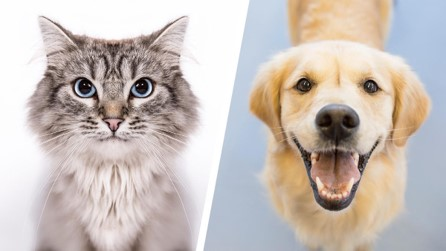
\includegraphics[width=0.4\textwidth]{images/cat_dog}
				\caption{Cat and dog comparison}
				\label{fig:cat_or_dog}
			\end{figure}

			\de{Lange Zeit galt die automatische Erkennung von Objekten, Personen und Szenen in Bildern durch Computer als unmöglich. Die Komplexität schien zu groß, als dass man sie einem Algorithmus programmatisch beibringen könnte. Bis noch vor einigen Jahrzehnten hat man so versucht Bildklassifikation durch manuell entwickelte Algorithmen zu erreichen. Die automatisierte Klassifikation anhand von vorgegebenen und vorklassifizierten Daten und dem automatisierten Erstellen von Modellen war ein neuer Schritt in eine neue Vorgehensweise. Die dabei immer mehr zur Verfügung stehende Rechenzeit spielt dabei genauso eine entscheidende Rolle am Erfolg wie parallelen Berechnungen auf mehreren \acp{gpu}, die Entwicklung effizienterer Algorithmen und Methoden wie \acl{da} und der Aufbau von Online-Datenbanken mit großen Mengen an beschrifteten Daten (ImageNet)\autocite{seif_deep_2019}. Mittlerweile ist die Bilderkennung ein weit verbreitetes Anwendungsgebiet des maschinellen Lernens. Häufig werden für Bilder sogenannte "\acp{cnn}\autocite{noauthor_convolutional_2020}" oder auch "ConvNets" verwendet.}
			\en{For a long time, the automatic recognition of objects, people and scenes in images by computers was considered impossible. The complexity seemed too great to be programmatically taught to an algorithm. Until a few decades ago, attempts were made to achieve image classification by manually developed algorithms. Automated classification based on given and pre-classified data sets and the automated creation of models was a new step into a new approach. The ever increasing amount of available computing time plays as much a decisive role in the success as parallel computations on several \acp{gpu}, the development of more efficient algorithms and methods such as \acl{da} and the establishment of online databases with large amounts of labeled data (ImageNet)\autocite{seif_deep_2019}. Meanwhile, image recognition has become a widespread application area of \ac{ml}. So-called "\acp{cnn}"\autocite{noauthor_convolutional_2020} or "ConvNets" are often used for images.}

			\de{Der Bildklassifizierungsalgorithmus nimmt ein Bild als Eingabe entgegen und klassifiziert es in eine der möglichen Ausgabekategorien. Der Ansatz Wissen aus bestehenden Daten zu lernen wird \acf{ml} genannt. In Verbindung mit \acfp{ann} nennt man es genauer \acf{dl}. Verschiedene \acfp{cnn}, wie ResNet, DenseNet, Inception, etc. wurden als hochpräzise Netzwerke für die Bildklassifikation entwickelt. Gleichzeitig wurden Bilddatensätze angelegt, um getaggte Bilddaten zu erfassen. Diese werden jetzt vorrangig dazu verwendet um bestehende Netzwerke zu trainieren und alljährliche Challenges zu veranstalten, welche sich mit den bisher bekannten und schon entwickelten Modellgenauigkeiten messen. ImageNet ist ein solch großer Datensatz mit mehr als 11 Millionen Bildern und über 11.000 Kategorien\autocite{noauthor_imagenet_2019}. Wenn ein Netzwerk einmal mit ImageNet-Daten trainiert wurde, kann es durch einfache Neuanpassung oder Optimierung mit anderen Datensätzen verallgemeinert werden. Bei diesem Transfer-Lernansatz wird ein Netzwerk mit Gewichten initialisiert, welche aus einem zuvor trainierten Netzwerk stammen. Dieses zuvor initialisierte Netzwerk wird nun für eine neue Bildklassifikationsaufgabe lediglich entsprechend angepasst.}
			\en{The image classification algorithm accepts an image as input and classifies it into one of the possible output categories. The approach to learn knowledge from existing data is called \acf{ml}\autocite{noauthor_machine_2020}. In combination with \acfp{ann} it is more precisely called \acf{dl}\autocite{noauthor_deep_2020}. Various \acfp{cnn}, such as ResNet, DenseNet, Inception, etc. have been developed as high-precision networks for image classification. At the same time, image data sets were created to capture tagged image data. These are now primarily used to train existing networks and to organize annual challenges that compete with the model accuracies already known and developed. ImageNet is such a large data set with more than 11 million images and over 11,000 categories\autocite{noauthor_imagenet_2019}. Once a network has been trained with ImageNet data, it can be generalized with other data sets by simple re-compilation or optimization. In this \acl{tl} approach, a network is initialized with weights that come from a previously trained network. This previously initialized network is now simply adapted for a new image classification task.}

			\de{Die hier zugrunde liegende Arbeit beschäftigt sich hauptsächlich mit überwachtem Lernen, bei dem ein mathematisches Modell aufgrund bestehender bekannter Datensätze trainiert wird. Das Ziel des trainierten Modells ist es dabei auch für unbekannte Bilder bestmögliche Vorhersagen zu treffen. Diese bekannten Datensätze werden meist händisch erstellt, automatisiert aufgrund bekannter Tatsachen bestimmt oder auch in einem halbautomatischen Prozess ermittelt.}
			\en{The underlying thesis here is mainly concerned with supervised learning, in which a mathematical model is trained based on existing known data sets. The purpose of the trained model is to make the best possible predictions even for unknown images. Known data sets are usually created manually, automatically determined based on known facts, or determined in a semi-automatic process.}



		% -------------------- %
		% Deductive approach %
		% -------------------- %
		\subsubsection{Deductive approach}
		\label{sec:section_deductive_approach}
			\de{Seit den späten 1960er Jahren hat man versucht, Bilder mit \textit{selbstgeschriebenen} Algorithmen zu klassifizieren. Dieser Teil der Computer Vision beschäftigt sich mit Techniken wie Bildentstehung, Bildbearbeitung und Bildsegmentierung. Im Bereich der Bildverarbeitung reihen sich bekannte Verfahren wie Kantenerkennungen, Merkmalsdetektoren, Randverknüpfungen, Kontrastverbesserungen, etc.\autocite{szeliski_computer_nodate} Allen Techniken gemein ist die Verwendung des deduktiven Ansatzes. Beim deduktiven Ansatz erstellt man Regeln (Merkmalsdetektoren), welche das gewünschte Ergebnis vorhersagen sollen. Diese Regeln werden vorgegeben und beschrieben und erlauben damit später eine Klassifizierung von unbekannten Objekten. Da das Modell und sein Algorithmus hinreichend bekannt ist, wird dieses Verfahren White-Box-Verfahren genannt.}
			\en{Since the late 1960s, attempts have been made to classify images with \textit{self-written} algorithms. This part of computer vision deals with techniques such as image creation, image processing and image segmentation. In the field of image processing, well-known techniques such as edge detection, feature detectors, edge linking, contrast enhancement, etc. are used\autocite{szeliski_computer_nodate}. Common to all techniques is the use of the deductive approach. With the deductive approach, one creates rules (feature detectors) which are supposed to predict the desired result. These rules are given and described and thus allow later classification of unknown objects. Since the model and its algorithm are sufficiently well known, this procedure is called a white-box procedure (Figure \ref{fig:overview_deductive_approach}).}

			\begin{figure}[H]
				\begin{center}
					\scalebox{1.0}{\includetex{deductive_approach}}
				\end{center}
				\caption{Deductive approach (the shown model is a white-box model)}
				\label{fig:overview_deductive_approach}
			\end{figure}



		% -------------------- %
		% Inductive approach %
		% -------------------- %
		\subsubsection{Inductive approach}
		\label{sec:section_inductive_approach}
			\de{Der induktive Ansatz hingegen verfolgt einen anderen Ansatz Bilder zu klassifizieren. Das Ziel ist nicht die Vorgabe einer Regel, sondern das Vorgehen aus schon bekannten einzelnen Objekten eine Regel (Modell) automatisiert zu erlernen\autocite{de1998machine}. Ein Modell meist eine komplexe Funktion und eine mathematische Abbildung eines Raumes (VC Dimension\autocite{noauthor_vapnikchervonenkis_2020}), in welcher einzelne Objekte mit ihren Eigenschaften abgebildet und getrennt werden können. Das Modell wird Stück für Stück den bekannten Objekten so angepasst, dass der Eingabewert dem Ausgabewert entspricht bzw. weitgehend entspricht (Backpropagation). Das Ziel ist es mit diesem Modell eine Funktion zu erstellen, welche in der Lage ist auch unbekannte Objekte bestmöglichst zu klassifizieren. Da der Raum dieses Modell meist fern der Vorstellungskraft und der Erklärungsmöglichkeit liegt, wird dieses Verfahren auch Black-Box-Verfahren genannt. Der hier beschriebene Vorgang wird meist bei jeder Art von \nameref{sec:section_supervised_classification} angewendet und ist ein Teil des \nameref{sec:section_machine_learning}.}
			\en{The inductive approach, on the other hand, takes a different approach to classifying images. The goal is not to specify a rule, but to learn a rule (model) automatically from already known individual objects\autocite{de1998machine}. A model is usually a complex function and a mathematical representation of a space, in which individual objects with their properties can be mapped and separated. This measure of the capacity that can be learned by this complex function is called \ac{vcd}\autocite{noauthor_vapnikchervonenkis_2020}. The model is adapted piece by piece to the known objects in such a way that the input value corresponds to the output value or corresponds to a large extent (backpropagation). The goal is to create a function with this model, which can classify unknown objects in the best possible way. Because the space of this model is mostly far away from the imagination and the possibility of explanation, this procedure is also called a black-box procedure (Figure \ref{fig:overview_inductive_approach}). The procedure described here is mostly used for any kind of supervised learning (see chapter ``\nameref{sec:section_supervised_learning}'') and is a part of \ac{ml} (see chapter ``\nameref{sec:section_machine_learning}'').}

			\begin{figure}[H]
				\begin{center}
					\scalebox{1.0}{\includetex{inductive_approach}}
				\end{center}
				\caption{Inductive approach  (the shown model is a black-box model)}
				\label{fig:overview_inductive_approach}
			\end{figure}



		% -------------------- %
		% Balanced training data set %
		% -------------------- %
		\subsubsection{Balanced training data set}
		\label{sec:section_balanced_training_data_set}
			\de{Neuronale Netze haben in den letzten Jahren \textit{enorme} Fortschritte im Bereich der Mustererkennung gemacht. Dabei ist ein entscheidender Faktor, dass die Daten zum Lernen eine hohe Qualität und eine einfache Verarbeitung für das Netzwerk aufweisen müssen. Falsch klassifizierte oder irrelevante Daten könnten dazu führen, dass das Netzwerk was Falsches lernt. Das gilt auch für eine nicht vorhandene bzw. nicht geeignete Vorverarbeitung.}
			\en{Neural networks have made \textit{enormous} progress in the field of pattern recognition in recent years. A decisive factor is that the data for learning must be of high quality and easy for the network to process. Wrongly classified or irrelevant data could cause the network to learn something wrong. This also applies to non-existent or unsuitable pre-processing\autocite{osinga2019data}.}

			\de{Mit dem Beginn eines Klassifizierungsprojektes stellt sich die Frage was genau man klassifizieren möchte und wie umfangreich die Klassifzierung ausfallen soll. Angenommen man möchte verschiedene Klassen von Essen identifizieren, so könnten das Klassen wie Pizza, Burger, Donuts und Lasagne sein (etc.). Zu diesen Klassen benötigt man nun eine große Anzahl an Bildern. Diese Daten sollten im Idealfall die Realität möglichst gut widerspiegeln. Eine große Variation ist von Vorteil (ausbalancierter Datenset): verschiedene Blickwinkel, Größe, Position, Farbhelligkeiten, Variationen, Anzahl, etc. Bilder von z.B. nur einer Farbhelligkeit oder nur einem Blickwinkel sollten vermieden werden. Sind die Daten nicht ausbalanciert, so müssen diese entsprechend korrigiert werden: z.B. durch Hinzufügen weiterer Daten, Bildverarbeitung oder durch Entfernen von Daten, welche für eine Unausgewogenheit sorgen. Weiterhin sollten die ausgewählten Klassen untereinander klar optisch trennbar sein. Sind sich zwei Klassen optisch sehr ähnlich und selbst durch einen Menschen nicht wirklich unterscheidbar, sollte darüber nachgedacht werden diese zusammenzufassen (z.B. "burger" und "veggie burger"):}
			\en{With the beginning of a classification project, the question arises what exactly one wants to classify and how extensive the classification should be. Assuming one wants to identify different classes of food, these could be classes like burgers (as shown in Figure \ref{fig:class_burger_doughnut_pizza}a), doughnuts (Figure \ref{fig:class_burger_doughnut_pizza}b) or pizza (Figure \ref{fig:class_burger_doughnut_pizza}c), etc. For these classes, one now needs a large number of images. Ideally, this data should reflect reality as far as possible. A large variation is advantageous (balanced data set): different viewing angles, size, position, colour brightness, variations, number, etc. Images of e.g. only one colour brightness or only one viewing angle should be avoided. If the data are not balanced, they must be corrected accordingly: e.g. by adding further data, image processing or by removing data that causes an imbalance. Furthermore, the selected classes should be clearly optically separable from each other. If two classes are visually very similar and not really distinguishable even by a human, consideration should be given to combining them (e.g. "burger" and "veggie burger").}

			\begin{figure}[H]
				\centering
				\begin{subfigure}[b]{1.025\textwidth}
					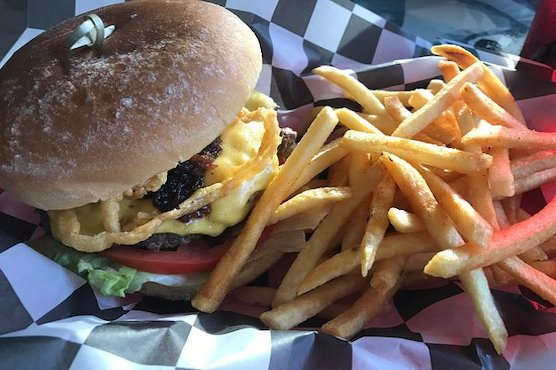
\includegraphics[width=0.19\textwidth]{images/data/burger2/1.jpg}
					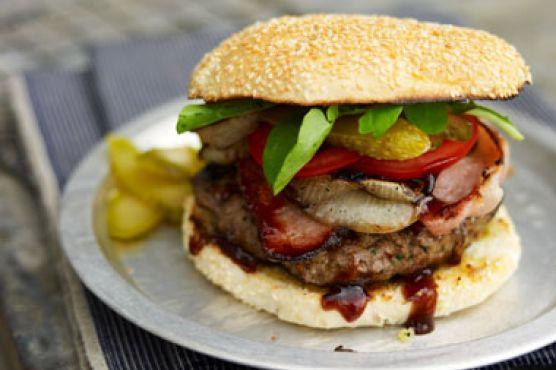
\includegraphics[width=0.19\textwidth]{images/data/burger2/2.jpg}
					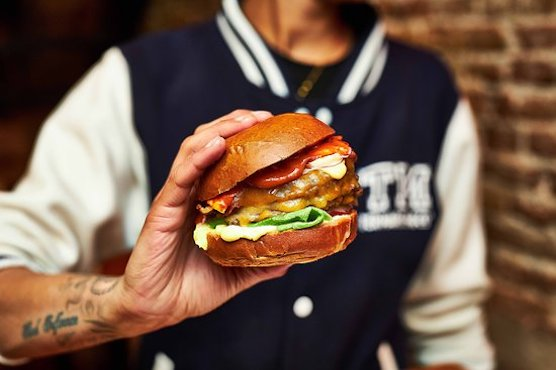
\includegraphics[width=0.19\textwidth]{images/data/burger2/3.jpg}
					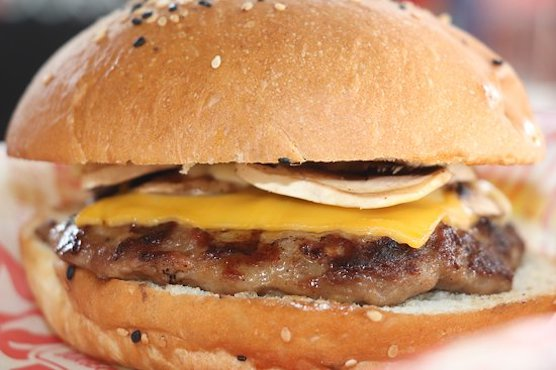
\includegraphics[width=0.19\textwidth]{images/data/burger2/4.jpg}
					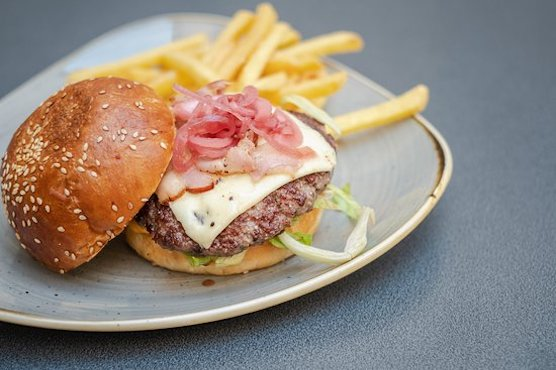
\includegraphics[width=0.19\textwidth]{images/data/burger2/5.jpg}
				\end{subfigure}

				\vspace{5pt}
				\begin{subfigure}[b]{1.025\textwidth}
					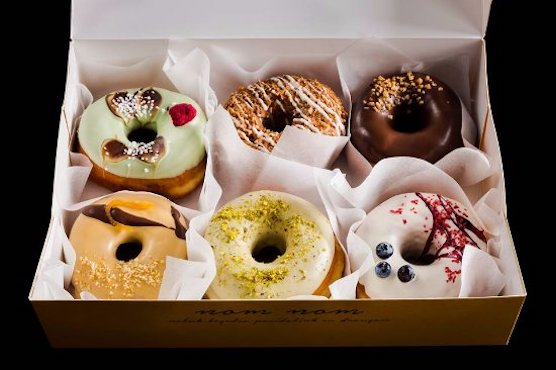
\includegraphics[width=0.19\textwidth]{images/data/donut2/1.jpg}
					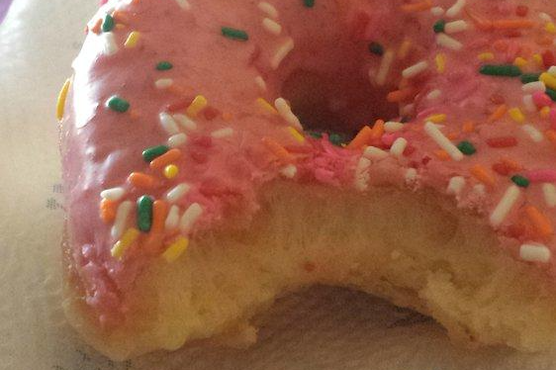
\includegraphics[width=0.19\textwidth]{images/data/donut2/2.png}
					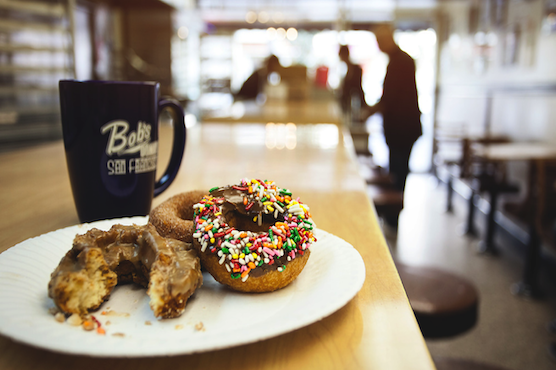
\includegraphics[width=0.19\textwidth]{images/data/donut2/3.png}
					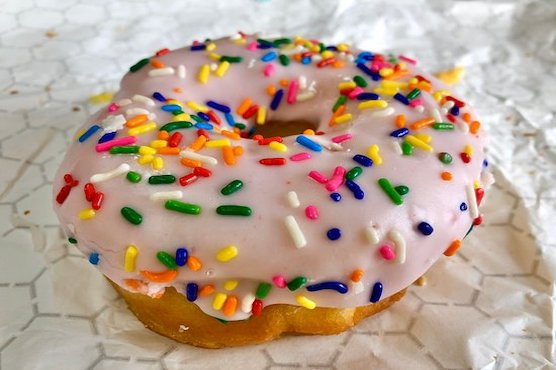
\includegraphics[width=0.19\textwidth]{images/data/donut2/4.jpg}
					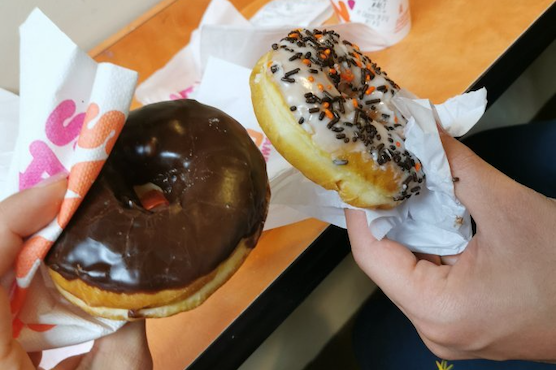
\includegraphics[width=0.19\textwidth]{images/data/donut2/5.png}
				\end{subfigure}

				\vspace{5pt}
				\begin{subfigure}[b]{1.025\textwidth}
					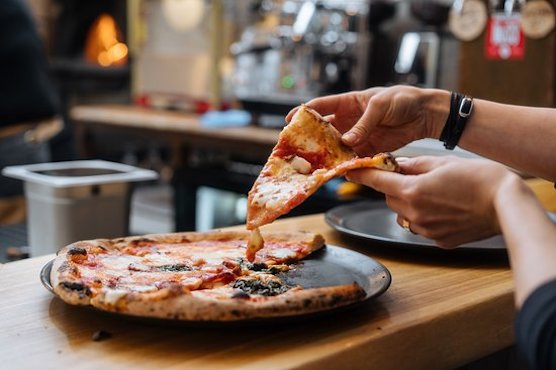
\includegraphics[width=0.19\textwidth]{images/data/pizza2/1.jpg}
					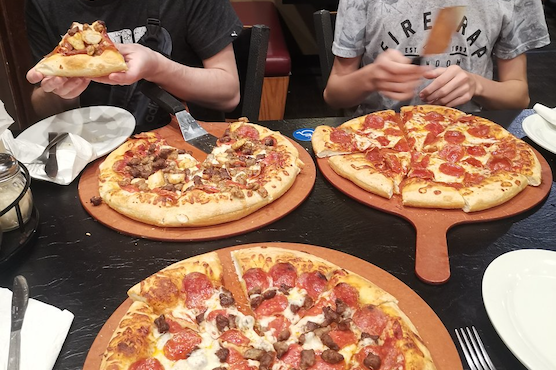
\includegraphics[width=0.19\textwidth]{images/data/pizza2/2.png}
					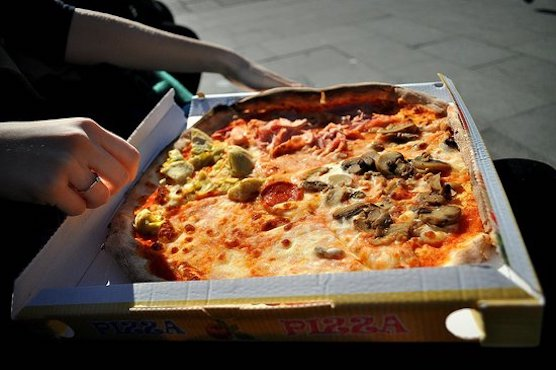
\includegraphics[width=0.19\textwidth]{images/data/pizza2/3.jpg}
					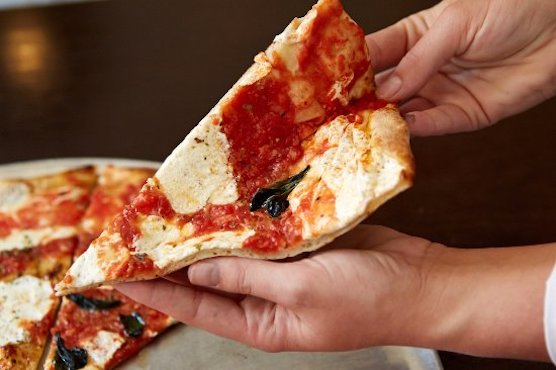
\includegraphics[width=0.19\textwidth]{images/data/pizza2/4.jpg}
					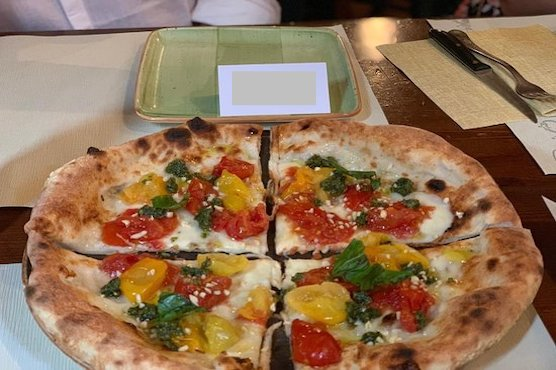
\includegraphics[width=0.19\textwidth]{images/data/pizza2/5.jpg}
       				\end{subfigure}
       				
				\caption[Example of pictures of a burger, doughnut and pizza class]{(a) Example of pictures of a burger class (top), (b) Example pictures of a doughnut class (middle), (c) Example of pictures of a burger class (bottom)}
				\label{fig:class_burger_doughnut_pizza}
			\end{figure}

			\de{An Daten zu gelangen ist oftmals nicht so einfach. Jede Datenquelle hat ihre eigenen Besonderheiten. Eine Möglichkeit an Daten zu gelangen wäre ein automatische Crawling von Bilddatenbanken (Flickr), Suchmaschinen (Google, Bing) oder Rezensionen (TripAdvisor), in welchen Bilder vorkommen und mit dem Text in Verbindung gebracht werden können (``Das hier ist der beste Donut, den ich je gegessen habe.''). Eine kreative Herangehensweise ist hier von Vorteil.}
			\en{Accessing data is often not that easy. Every data source has its own special features. One way to access data would be an automatic crawling of image databases (Flickr\autocite{noauthor_flickr_nodate}), search engines (Google\autocite{noauthor_google_nodate}, Bing\autocite{noauthor_bing_nodate}) or reviews (TripAdvisor), in which images appear and can be associated with the text (``This here is the best doughnut I've ever eaten.''). A creative approach is an advantage here.}
			
			\de{Die wahrscheinlich teuerste Variante an Daten zu gelangen ist die händische Suche und Klassifizierung durch z.B. einen Ontologen. Dieser beurteilt und sucht verschiedenen Bilder und ordnet diese händisch in die entsprechenden Klassen ein. Auch eine kombinierte Variante ist möglich und wahrscheinlich zu bevorzugen: Automatisches Crawling und händisches aussortieren falscher, ungünstiger oder irrelevanter Bilder.}
			\en{Probably the most expensive way to obtain data is to search and classify them manually, e.g. by an ontologist. The ontologist evaluates and searches for different images and manually classifies them in the appropriate classes. A combined variant is also possible and probably preferable: automatic crawling and manual sorting out of incorrect, unfavorable or irrelevant images.}

		% -------------------- %
		% Training, validation and test data set %
		% -------------------- %
		\subsubsection{Training, validation and test data set}
		\label{sec:section_training_test_and_evaluation}
			\de{Vor dem Beginn mit dem Training von ausbalancierten Bildern müssen diese in einen Trainings-, einen Test- und eventuell in einen Validierungsdatensatz aufgeteilt werden. Dies ist notwendig, da neuronale Netze zu einem Teil nicht verallgemeinern, sondern auswendig lernen werden (overfitting\autocite{noauthor_overfitting_2020}). Die Idee ist es mit einem Trainingsdatensatz zu trainieren, während mit dem Validierungsdatensatz die Allgemeingültigkeit des Netzes und seiner Parameter überwacht wird. Anhand der Ergebnisse werden zur Laufzeit Anpassungen vorgenommen. Da die Anpassung der Parameter anhand der Testdaten vorgenommen wird, gibt es noch einen unabhängigen Testdatensatz, welcher eine erneute Überprüfung des Modells auf bisher unbeteiligte Daten vornimmt. Dieser stellt sicher, dass nicht versehentlich Hyperparameter nur speziell für den Validierungsdatensatz optimiert werden\autocite{osinga2019data}. Die Verwendung des Testdatensatz ist optional und simuliert das Modell unter realen Bedingungen. Ist die Anzahl der Daten begrenzt und kann dieser Datensatz z.B. auch dem Trainingsdatensatz hinzugefügt werden. In dieser Arbeit wird auf den Testdatensatz verzichtet und sämtliche Auswertungen beziehen sich auf den Validierungsdatensatz.}
			\en{Before starting the training of balanced images, they must be divided into a training, a test and possibly a validation data set. This is necessary because \acp{nn} will not generalize to some extent, but will learn by heart (overfitting\autocite{noauthor_overfitting_2020}). The idea is to train with a training data set, while the validation data set is used to monitor the general validity of the network and its parameters. Based on the results, adjustments are made at runtime. Since the adjustment of the parameters is carried out using the test data, there is also an independent test data set, which carries out a renewed check of the model for previously uninvolved data. This ensures that hyperparameters are not inadvertently optimized for the validation data set only\autocite{osinga2019data}. The use of the test data set is optional and simulates the model under real conditions. If the number of data is limited, this data record can also be added to the training data record, for example. In this thesis, the test data set is not used and all evaluations refer to the validation data set.}

			\de{Eine optimale Aufteilung des Trainings- und Validierungsdatensatzes ist abhängig von dem vorliegenden Klassifizierungsproblem und die Anzahl der Daten, welche zur Verfügung stehen. In dieser Arbeit wird nach dem Pareto Prinzip ein Verhältnis aus 80\% Trainingsdaten und 20\% Validierungsdaten verwendet, sofern nicht anders angegeben.}
			\en{An optimal division of the training and validation data set depends on the existing classification problem and the amount of data available. In this thesis a ratio of 80\% training data and 20\% validation data is used according to the Pareto principle, unless otherwise stated.}



	% -------------------- %
	% Classification Metrics %
	% -------------------- %
	\subsection{Classification metrics and confusion matrix}
		\de{Die Wahl der richtigen Metrik ist bei der Bewertung von Modellen des maschinellen Lernens von entscheidender Bedeutung. Metriken werden zur Überwachung und Messung der Leistung eines Modells während des Trainings und des Tests verwendet. Im nachfolgenden werden einige wichtige Metriken erklärt.}
		\en{Choosing the right metric is crucial in evaluating \ac{ml} models. Metrics are used to monitor and measure the performance of a model during training and testing. Some important metrics are explained below.}



		% -------------------- %
		% loss function %
		% -------------------- %
		\subsubsection{Loss function}
		\label{sec:section_loss_function}
			\de{Für die Klassifikation eines Bildes \(\vartheta\) wird in der Regel ein neuronales Netzwerk verwendet. Die Funktion für dieses Modell werde mit \(\boldsymbol M(\vartheta)\) angegeben. Bei diesem Model ist letzte Schicht eines Klassifikators auf Basis eines neuronalen Netzes meist eine Softmax Funktion\autocite{noauthor_softmax_2019}. Dabei wird einem Element ein Vektor \(\lambda\) der Größe \(n\) zugewiesen und ist der vorhergesagter Wert \(\boldsymbol\lamda\) von diesem Element. Die Größe \(n\) entspricht dabei der Anzahl der zu unterscheidenden Klassen\autocite{geron2017supervisedlearningDecisionBoundaries}. Jeder einzelne \(p\) Wert entspricht dabei der Wahrscheinlichkeit, dass es sich um die Klasse \(class_n\) handelt (Gleichung \ref{eq:equation_softmax_vector}).}
			\en{For the classification of an image \(\vartheta\) a \ac{nn} is usually used. The function for this model is specified with \(\boldsymbol M(\vartheta)\). In this model the last layer of this \ac{nn}-based classifier is mostly a softmax function\autocite{noauthor_softmax_2019}. It assigns a vector \(\boldsymbol\lambda\) of size \(n\) to an element \(\vartheta\) and is the predicted value of this element. The size \(n\) corresponds to the number of classes to be distinguished\autocite{geron2017supervisedlearningDecisionBoundaries}. Each individual value \(p\) of \(\boldsymbol\lambda\) corresponds to the probability that it is class \(class_n\) (Equation \ref{eq:equation_softmax_vector}).}

			\begin{equation}
				\boldsymbol M(\vartheta) =
				\boldsymbol\lambda = 
				\left(
					\begin{array}{c}
					p_{1}\\
					p_{2}\\
					p_{3}\\
					\vdots\\
					p_{n}\\
					\end{array}
				\right)
				\quad\Biggl\lvert \quad \sum_{i=1}^n p_i = 1
				\label{eq:equation_softmax_vector}
			\end{equation}

			\de{Der erwartete Wert der Parameterfunktion und somit der aktuellen Klasse wird als One Hot Vektor zurückgegeben. Der Wert 1 entspricht der erwarteten Klasse. Alle anderen Klassen geben 0 zurück. Dies nennt man auch One Hot Encoding (am Beispiel von Klasse 2):}
			\en{The expected value of the parameter function \(\boldsymbol g(\vartheta)\) and thus of the current element \(\vartheta\) and its expected labelled class is returned as a so-called "one-hot vector". The vector element for the expected class has the value 1, all others have the value 0. This is also called one hot encoding (using the example of an element of \(class_2\)):}

			\begin{equation}
				\boldsymbol g(\vartheta_{class_2}) = 
				\left(
					\begin{array}{c}
					0\\
					1\\
					0\\
					\vdots\\
					0\\
					\end{array}
				\right)
			\end{equation}

			\de{Die Verlustfunktion\autocite{noauthor_verlustfunktion_2018} ordnet jeder Vorhersage einen Schaden zu, der durch den Vergleich mit dem wahren Wert bzw. Parameter entsteht. Backpropagation berechnet den Gradienten der Verlustfunktion, welcher mit \(m(\vartheta)\) entsteht. Dazu wird der Abstand der vorhergesagten Klasse zur wahren Klasse berechnet (sind sie gleich ist der Abstand 0). Bessert sich mit Anpassung des Modells (Lernvorgang) die Vorhersage aller vorhergesagten Klassen zu ihren wahren Klassen, so verkleinert sich auch der Wert der Verlustfunktion. Eine typische Verlustfunktion ist z.B. für einen r-dimensionalen Raum:}
			\en{The loss function\autocite{noauthor_verlustfunktion_2018} assigns a loss to each prediction \(\boldsymbol\lambda\), which results from the comparison with the true value of the parameter function \(\boldsymbol g(\vartheta_{class})\). Backpropagation (see chapter ``\nameref{sec:section_backpropagation}'') calculates for each element \(\vartheta\) the gradient of the loss function which results with \(\boldsymbol M(\vartheta)\). The gradient is used to adapt the parameters of function \(\boldsymbol M(\vartheta)\) to reduce the prediction error. If the adaptation of the model improves the prediction of an element to its true value, the value of the loss function is also reduced. As an example, a typical loss function for an r-dimensional space for one element is shown in Equation \eqref{eq:equation_loss_function}.}

			\begin{equation}
				\label{eq:equation_loss_function}
				L_r(\vartheta, \boldsymbol\lambda) := \lVert \boldsymbol\lambda - \boldsymbol g(\vartheta) \rVert^r
			\end{equation}

			\de{\(\lambda\) stellt hierbei den geschätzte Wert und \(g(\vartheta)\) die Parameterfunktion dar, welche den realen Wert für \(\vartheta\) zurückliefert. Der mittlere Verlust auf den gesamten Datensatz mit \(n\) Elementen ist somit:}
			\en{\(\boldsymbol\lambda\) represents the estimated value and \(g(\vartheta)\) the parameter function which returns the actual value for \(\vartheta\). The loss function is not only determined for one element. It is necessary to consider all elements together to create a model that generalises. The average loss on the entire data set with \(k\) elements is thus:}

			\begin{equation}
				\hat{L} = {{1}\over{k}}\sum_{i=1}^{k} L_r(\vartheta_i, \boldsymbol\lambda_i)
			\end{equation}



		% -------------------- %
		% Confusion Matrix %
		% -------------------- %
		\subsubsection{Confusion matrix}
		 	\de{Die Confusion Matrix ist eine spezielle quadratische Matrix auf dem Gebiet des maschinellen Lernens, das die Visualisierung der Leistung eines Vorhersage-Modells ermöglicht. Jede Zeile der Matrix repräsentiert die tatsächliche Klasse, während in jeder Spalte die Anzahl der entsprechend vorhergesagten Klassen angegeben werden (oder umgekehrt). Es wird eine spezielle Klasse \(class_1\) betrachtet: \ac{tp} entspricht dabei dem Wert der richtig ermittelten Vorhersagen der aktuell betrachteten Klasse. \ac{fn} gibt an, wie oft die aktuell betrachtete Klasse falsch ermittelt wurde. \ac{fp} gibt an, wie oft andere Klassen als die aktuell betrachtete Klasse ermittelt wurden. \ac{tn} wiederum gibt an, dass andere Klassen als die aktuelle Klasse auch richtig als andere Klassen vorhergesagt wurden\autocite{noauthor_confusion_2020-1}.}
		 	\en{The confusion matrix is a special quadratic matrix in the field of \ac{ml} that allows the visualization of the performance of a predictive model (Figure \ref{tbl:figure_confusion_matrix_1}). Each row of the matrix represents the actual class, while each column indicates the number or a numerical value as a percentage of the predicted class (or vice versa). A special class \(class_1\) is considered: \Ac{tp} corresponds to the value of the correctly determined predictions of the class currently under consideration. \Ac{fn} indicates how often other classes are detected as the class currently under consideration. \Ac{fp} indicates how often classes other than the currently viewed class were determined. \Ac{tn} in turn indicates that classes other than the current class were correctly predicted as the other classes\autocite{noauthor_confusion_2020-1}.}

			\begin{table}[htb]
				\centering
				\scalebox{0.75}{
					{\def\arraystretch{2}\tabcolsep=5pt
						\begin{tabular}{cc|c|c|c|c|}
							\cline{3-6}
							& & \multicolumn{4}{c|}{\textbf{predicted}} \\ \cline{3-6} 
							& & \boldmath\(class_1\) & \boldmath\(class_2\) & \textbf{\ldots} & \boldmath\(class_n\) \\ \hline
							\multicolumn{1}{|l|}{\multirow{4}{*}{\rotatebox{90}{\textbf{actual}}}} & \boldmath\(class_1\) & \(TP\)                  & \multicolumn{3}{c|}{\(FN\)} \\ \cline{2-6} 
							\multicolumn{1}{|c|}{} & \boldmath\(class_2\) & \multirow{3}{*}{\(FP\)} & \multicolumn{3}{c|}{\multirow{3}{*}{\(TN\)}} \\ \cline{2-2}
							\multicolumn{1}{|c|}{} & \textbf{\ldots} & & \multicolumn{3}{c|}{}                   \\ \cline{2-2}
							\multicolumn{1}{|c|}{} & \boldmath\(class_n\) & & \multicolumn{3}{c|}{}                   \\ \hline
						\end{tabular}
					}
				}
				\captionof{figure}{Confusion matrix}\label{tbl:figure_confusion_matrix_1}
			\end{table}

		 	\de{Zum Schluß besitzt die Confusion Matrix folgenden Aufbau (Gleichung \ref{eq:equation_confusion_matrix}), wobei die Anzahl von Elementen in der Klasse \(P_{i}\) vorhergesagt wurde, obwohl (\(\cong\)) es hätte Klasse \(A_{j}\) sein müssen. Alle Werte auf der Diagonalen wurden richtig vorhergesehen. Wenn das Modell eine Modellgenauigkeit von 100\% aufweist, dann wurden alle Klassen richtig vorhergesagt und alle Elemente neben der Hauptdiagonalen sind 0 (equation \ref{eq:equation_confusion_matrix_correct}).}
			\en{Finally, the confusion matrix has the following structure (Equation \eqref{eq:equation_confusion_matrix}). \(P_{i,j}\) means \(class_i\) was predicted although it should have been class \(class_j\). All values on the main diagonal were correctly predicted (\(P_{i,i}\)). \(\#P_{i,j}\) in turn is the total number that \(class_i\) was recognized, although it should be \(class_j\). If the model has a model accuracy of 100\%, there are values greater than 0 only on the main diagonal and all other non-diagonal elements are 0 (Equation \eqref{eq:equation_confusion_matrix_correct}).}

			\begin{equation}
				\boldsymbol{M}_{confusion} = \begin{bmatrix}
					\#P_{1,1} & \dots & \#P_{n,1} \\
					\vdots & \ddots & \vdots \\
					\#P_{1,n} & \dots & \#P_{n,n}
				\end{bmatrix} = (m_{nn})
				\label{eq:equation_confusion_matrix}
			\end{equation}

			\begin{equation}
				\boldsymbol{M}_{confusion} = \begin{bmatrix}
					\#P_{1,1} & \dots & 0 \\
					\vdots & \ddots & \vdots \\
					0 & \dots & \#P_{n,n}
				\end{bmatrix} = (m_{nn})
				\label{eq:equation_confusion_matrix_correct}
			\end{equation}

		% -------------------- %
		% Accuracy %
		% -------------------- %
		\subsubsection{Accuracy}
			\de{Die \textbf{Top-1-Genauigkeit} ist wahrscheinlich die wichtigste Genauigkeit. Sie sagt sagt aus, zu wieviel Prozent die jeweils beste Aussage des Modells auf die Daten des Validierungssets mit der erwarteten Klasse übereinstimmt.}
			\en{\textbf{Top-1 accuracy} is probably the most important accuracy. It tells one the percentage of the model's best prediction of the data in the validation set that matches the expected class.}

			\begin{equation}
				Accuracy = {{TP + TN} \over {TP + TN + FP + FN}} = {{\sum_{i,j=1}^{n} m_{ij}} \over {\sum_{i=1}^{n} \sum_{j=1}^{n} m_{ij}}} = {{Correct_{all}} \over {CorrectPossible_{all}}}
			\end{equation}

			\de{Die \textbf{Top-5-Genauigkeit} ist eine weitere Genauigkeitsangabe. Jedoch wird hier nicht nur der beste Treffer einbezogen, sondern auch die nächsten weiteren vier. Sobald die richtige Klasse innerhalb der ersten fünf vorhergesagten Klassen gefunden werden kann, so ist auch diese Vorhersage wahr:}
			\en{The \textbf{Top 5 Accuracy} is another accuracy specification. However, not only the best hit is included here, but also the next four. As soon as the correct class can be found within the first five predicted classes, this prediction is also true:}
			
			\begin{equation}
				Accuracy_{top-5} = {{CorrectWithinTheBest5Classes_{all}} \over {CorrectPossible_{all}}}
			\end{equation}

			\de{Die Genauigkeit des gesamten Modells ist eine gute Aussagekraft über die Leistungsfähigkeit des Modells. Ein Problem tritt jedoch in Extremfällen auf, bei denen nicht mehr zuverlässig Annahmen gemacht werden können. Zum Beispiel wenn man es mit einem unbalancierten Datensatz zu tun hat\autocite{geron2017supervisedlearningConfusionMatrix}. Beispiel: Angenommen man hätte ein Modell, dass immer die Klasse \(class_1\) vorhersagt. Die Klasse \(class_1\) besteht aus 9990 Elementen und von den anderen Klassen \(class_2\) bis \(class_n\) hat man genau 10. Dann sieht die Confusion Matrix wie in nachfolgender Abbildung aus.}
			\en{The accuracy of the entire model is a good indication of the performance of the model. However, a problem occurs in extreme cases where assumptions can no longer be made reliably. For example, if one is working with an unbalanced dataset\autocite{geron2017supervisedlearningConfusionMatrix}. Example: Suppose one has a model that always predicts the class \(class_1\). The class \(class_1\) consists of 9,990 elements and from the other classes \(class_2\) to \(class_n\) one has exactly 10. Then the confusion matrix looks like in the following figure (Figure \ref{tbl:figure_confusion_matrix_2}).}

			%\clearpage
			\begin{table}[htb]
				\centering
				\scalebox{0.75}{
					{\def\arraystretch{2}\tabcolsep=5pt
						\begin{tabular}{cc|c|c|c|c|}
							\cline{3-6}
							& & \multicolumn{4}{c|}{\textbf{predicted}} \\ \cline{3-6} 
							& & \boldmath\(class_1\) & \boldmath\(class_2\) & \textbf{\ldots} & \boldmath\(class_n\) \\ \hline
							\multicolumn{1}{|l|}{\multirow{4}{*}{\rotatebox{90}{\textbf{actual}}}} & \boldmath\(class_1\) & \(TP = 9990\)                  & \multicolumn{3}{c|}{\(FN = 0\)} \\ \cline{2-6} 
							\multicolumn{1}{|c|}{} & \boldmath\(class_2\) & \multirow{3}{*}{\(FP = 10\)} & \multicolumn{3}{c|}{\multirow{3}{*}{\(TN = 0\)}} \\ \cline{2-2}
							\multicolumn{1}{|c|}{} & \textbf{\ldots} & & \multicolumn{3}{c|}{}                   \\ \cline{2-2}
							\multicolumn{1}{|c|}{} & \boldmath\(class_n\) & & \multicolumn{3}{c|}{}                   \\ \hline
						\end{tabular}
					}
				}
				\captionof{figure}{Confusion matrix example}\label{tbl:figure_confusion_matrix_2}
			\end{table}

			\de{Die Modell-Genauigkeit ist ein ist in diesem Fall 99,9\%, obwohl es ein schlechtes Modell ist:}
			\en{The model accuracy in this case is 99.9\%, although it is a bad model:}

			\begin{equation}
				Accuracy = 99,9\%
			\end{equation}

			\de{Deswegen gibt es weitere Performance Metriken wie Precision, Recall und F-Measure.}
			\en{Therefore there are additional performance metrics like Precision, Recall and F-Measure.}

		% -------------------- %
		% Precision %
		% -------------------- %
		\subsubsection{Precision}
			\de{Precision\autocite{noauthor_precision_2020} sagt aus, wie zuverlässig die Aussage einer Vorhersage einer Klasse ist:}
			\en{Precision\autocite{noauthor_precision_2020} expresses how reliable the statement of a prediction of a class is:}

			\begin{equation}
				Precision = {{Correct} \over {Actual}} = {{TP} \over {TP + FP}}
			\end{equation}

			\de{Oder genauer für die Klasse c:}
			\en{Or more precisely for class c:}

			\begin{equation}
				Precision_{@c} = {{m_{cc}} \over {\sum_{i=1}^{n} m_{ic}}}
			\end{equation}

		% -------------------- %
		% Recall %
		% -------------------- %
		\subsubsection{Recall}
			\de{Recall\autocite{noauthor_precision_2020} ist die Genauigkeit einer Klasse. Das bedeutet wie gut konnte die Klasse vorhergesehen werden:}
			\en{Recall\autocite{noauthor_precision_2020} is the accuracy of a class. This means how well the class could be predicted:}

			\begin{equation}
				Recall = {{Correct} \over {CorrectPossible}} = {{TP} \over {TP + FN}}
			\end{equation}

			\de{Oder genauer für die Klasse c:}
			\en{Or more precisely for class c:}

			\begin{equation}
				Recall_{@c} = {{m_{cc}} \over {\sum_{i=1}^{n} m_{ci}}}
			\end{equation}

		% -------------------- %
		% F-Measure %
		% -------------------- %
		\subsubsection{F-Measure}
			\de{F-Measure\autocite{noauthor_f1_2020} kombiniert Präzision und Rückruf, wobei der Parameter \(\beta\) die Gewichtung darstellt:}
			\en{F-Measure\autocite{noauthor_f1_2020} combines precision and recall, with the parameter \(\beta\) representing the weighting:}
			\begin{equation}
				F_\beta =
				(1 + \beta^2) \cdot {{Precision\cdot Recall}\over{\beta^2 \cdot Precision + Recall}} = 
				{{(1 + \beta^2) \cdot TP}\over{(1 + \beta^2) \cdot TP + \beta^2 \cdot FN + FP}}
			\end{equation}

			\de{Je höher der \(\beta\), desto mehr Wert wird auf Precision statt auf Recall gelegt. Das ist wichtig, wenn man mehr Wert auf die Qualität der Verhersage legt, als auf die Erkennungsgenauigkeit. Z.B. bei einer Vorhersage von Krankheiten: Zuordnung von Klasse Krank bei gesunden Menschen ist hier genauso fatal wie auch die Zuordnung von Klasse Gesund bei kranken Menschen. Mit einem Wert von \(\beta = 0,5\) erhält man eine Gleichverteilung beider Werte und wird F1 score genannt:}
			\en{The higher \(\beta\) the more importance is placed on precision instead of recall. This is important if one puts more importance on the quality of the prediction than on the accuracy of prediction. For example, when predicting diseases: assigning class ``ill'' to healthy people is just as fatal as assigning class ``healthy'' to sick people. A value of \(\beta = 0.5\) one gets an equal distribution of both values and is called F1 score:}

			\begin{equation}
				F_1 =
				{{2 \cdot Precision \cdot Recall}\over{Precision + Recall}} = 
				{{2 \cdot TP}\over{2 \cdot TP + FN + FP}}
			\end{equation}

		\subsection{Machine learning}
		\label{sec:section_machine_learning}
			\de{Maschinelles Lernen ist ein Oberbegriff für die künstliche Generierung von Wissen aus Erfahrung\autocite{de1998machine}. Es verfolgt den Ansatz des induktiven Lernens (siehe auch Kapitel \nameref{sec:section_inductive_approach}).}
			\en{Machine learning is a generic term for the artificial generation of knowledge from experience\autocite{de1998machine}. It follows the approach of inductive learning (see also chapter \nameref{sec:section_inductive_approach}).}
			
			
			
			% -------------------- %
			% Short definitions %
			% -------------------- %
			\subsubsection{Short definitions}
			\label{sec:section_short_definitions}

				\paragraph{Backpropagation}
				\label{sec:section_backpropagation}
					\hl{...}
					
				\paragraph{Batch size}
				\label{sec:section_batch_size}
					\de{Die Batch Size definiert die Anzahl der Bilder, die gleichzeitig vorwärts und rückwärts durch das neuronale Netzwerk geleitet werden, bevor die Parameter im Netzwerk angepasst werden (Gradientenaktualisierung). Normalerweise ist es pro Epoche vorgesehen alle Trainingsdaten mit einem Vorgang zu trainieren. Dies ist gerade im Bereich der Bildklassifizierung aufgrund des begrenzten Speichers meist nicht möglich, weshalb man eine Epoche in viele kleine Batches aufteilt (Mini-Batches). Der Vorteil besteht darin, dass man nur die Daten im Speicher halten muss, die für den aktuellen Batch nötig sind und damit eine Überanpassung reguliert werden kann. Der Nachteil ist eine erhöhte Varianz (Rauschen in der Genauigkeit des Modells), da es unwahrscheinlich ist, dass eine kleine Stichprobe eine gute Darstellung des gesamten Datensatzes ist. Ebenso erhöht sich der Rechenaufwand da die Backpropagation entsprechend der Anzahl der Mini-Batches erhöht. Es gibt keine magische Regel für die richtige Wahl der Batch Size. Dies ist ein Hyperparameter, der vor Beginn des Trainings bestimmt werden muss\autocite{noauthor_epochs_nodate}.}
					\en{The batch size defines the number of images that are simultaneously passed forward and backward through the \ac{nn} before the parameters in the network are adjusted (gradient update). Normally it is intended to train all training data per epoch with one process. Especially in the field of image classification this is usually not possible due to the limited memory, which is why an epoch is divided into many small batches (mini-batches). The advantage is that one only has to keep the data in memory that is necessary for the current batch and an overfitting can be regulated.  The disadvantage is an increased variance (noise in the accuracy of the model), since it is unlikely that a small batch is a good representation of the entire data set. The computing time increases as well, since the backpropagation increases according to the number of mini-batches. There is no magic rule for choosing the right batch size. This is a hyperparameter that must be determined before the training begins\autocite{noauthor_epochs_nodate}.}

				\paragraph{Class}
				\label{sec:section_class}
					\hl{...}

				\paragraph{Data augmentation}
				\label{sec:section_data_augmentation}
					\de{Als Data Augmentation bezeichnet man die künstliche Vergrößerung eines Datensets. Diese Technik wird vorrangig dann angewendet, wenn man nur wenig Daten zur Verfügung hat oder das Datenset nicht ausreichend balanciert ist. Dabei werden bestehende Bilder gedreht, gespiegelt, Farbkorrekturen vorgenommen, ausgeschnitten, etc. Die Data Augmentation kann die Modellgenauigkeit beim Training verbessern\autocite{perez2017effectiveness}.}
					\en{Data augmentation is the artificial augmentation of a data set. This technique is primarily used when only little data is available or the data set is not sufficiently balanced (unbalanced data set). Existing images are rotated, mirrored, color adjusted, cropped, etc. Data Augmentation can improve model accuracy during training\autocite{perez2017effectiveness}.}

				\paragraph{Dropout}
				\label{sec:section_dropout}
					\hl{...}

				\paragraph{Learning epoch}
				\label{sec:section_learning_epoch}
					\de{Unter einer Lernepoche versteht man den einmaligen Trainingsdurchlauf mit allen Trainingsdatensätzen. Meist reicht ein Trainingsdurchlauf nicht aus, weshalb weitere Lernepochen im Anschluß erfolgen. Sobald mit weiteren Lernepochen die Leistungsfähigkeit des Netzwerkes nicht weiter steigt, beendet man das Training.}
					\en{A learning epoch is understood to be the one time training run with all training data sets. Usually one training run is not sufficient, which is why further learning epochs follow. As soon as the performance of the network does not increase anymore with further epochs, the training is terminated.}
					
				\paragraph{Learning rate}
				\label{sec:section_learning_rate}
					\de{Die Lernrate ist ein Abstimmungsparameter in einem Optimierungsalgorithmus. Dieser sagt aus, wie groß die Schrittweite bei jeder Iteration ist, mit der sich die Parameter auf das Minimum einer Verlustfunktion zubewegen. Sie sollte nicht zu hoch (Minimum wird nicht gefunden) und nicht zu klein sein (sehr langsames Lernen). Die Lernrate wird oft mit dem Zeichen \(\eta\) oder \(\alpha\) bezeichnet.}
					\en{The learning rate is a tuning parameter in an optimization algorithm. It expresses how large the step size is for each iteration with which the parameters move closer to the minimum of a loss function. It should not be too high (minimum is not found) and not too small (very slow learning). The learning rate is often indicated by the character \(\eta\) or \(\alpha\).}

				\paragraph{Momentum}
				\label{sec:section_momentum}
					\hl{...}
			
			
			% -------------------- %
			% Methods of machine learning %
			% -------------------- %
			\subsubsection{Methods of machine learning}
			\label{sec:section_methods_of_machine_learning}
				\de{Je nach Art und Vorgehensweise der Überwachung des Trainings lassen sich verschiedene Machine-Learning-System einordnen. Dabei wird unterschieden, welche Art von Daten uns vorliegen oder diese selbst bestimmt werden müssen.}
				\en{Different \ac{ml} systems can be classified according to the type and procedure of monitoring the training. A distinction is made as to which type of data is available or has to be determined by the user.}
	
				% -------------------- %
				% Supervised learning %
				% -------------------- %
				\paragraph{Supervised learning}
				\label{sec:section_supervised_learning}
					\de{Das überwachte Lernen bezieht sich auf ein maschinelles Lernen mit bekannten Trainingsdatensätzen (siehe auch Kapitel ``\nameref{sec:section_inductive_approach}''). Der Lernprozess wiederrum bezieht sich auf die Fähigkeit einer künstlichen Intelligenz, Regelmäßigkeiten und Muster zu reproduzieren. Die Ergebnisse sind durch Naturgesetze oder Expertenwissen bekannt und werden für die Lehre des Systems verwendet, in dem ein Trainingsset erstellt wird, welcher die gewünschten Lösungen enthält. Man nennt dies auch gelabelte Daten. Der Lernalgorithmus versucht nun epochenweise eine Hypothese zu finden, die eine möglichst genaue Vorhersagen auf unbekannten Daten ermöglicht. Eine Hypothese ist in diesem Fall ein Bild, das jedem Eingabewert (das Bild selbst) den angenommenen Ausgabewert (die vorhergesagte Klasse) zuordnet. Diese Arbeit macht ausgiebigen Gebrauch von überwachtem Lernen.}
					\en{Supervised learning refers to \ac{ml} with known training data sets (see also chapter ``\nameref{sec:section_inductive_approach}''). The learning process in turn refers to the ability of an \ac{ai} to reproduce regularities and patterns. The results are known by laws of nature or expert knowledge and are used to teach the system by creating a training set containing the desired solutions. This is also called labelled data. The learning algorithm now tries to find a hypothesis epoch by epoch, which allows the most accurate predictions on unknown data. A hypothesis in this case is an image that assigns the assumed output value (the predicted class) to each input value (the image itself). This thesis makes extensive use of supervised learning.}
		
					\de{Beim Überwachten Lernen wird einer Klassifizierungsfunktion (meist ein künstliches neuronales Netz) ein Eingangsvektor zugeführt. Der Eingangsvektor erzeugt mit Hilfe der Klassifizierungsfunktion einen Ausgabevektor, die dieses neuronale Netz in seinem aktuellen Zustand produziert\footnote{Das neuronale Netzwerk besteht aus vielen (meist Millionen) Parametern, welche während des Lernprozesses angepasst werden können, um den Fehler zu minimieren.}. Dieser Wert wird mit dem Wert verglichen, den es eigentlich ausgeben soll. Der Vergleich des Soll- und Istzustandes gibt Auskunft wie und in welcher Form Änderungen am Netzwerk vorgenommen werden müssen, um dem Istzustand weiter anzugleichen und den Fehler zu minimieren. Für künstliche neuronale Netzwerke ohne versteckter Schicht (einlagiges Perzeptron\autocite{noauthor_perceptron_2020}) kann die Delta-Regel\autocite{noauthor_least_2020} für die Korrektur vorgenommen werden. Bei Netzwerken mit einer oder mehreren versteckten Schichten verwendet man Backpropagation\autocite{noauthor_backpropagation_2020} um den Fehler zu minimieren. Backpropagation ist eine Verallgemeinerung der Delta-Regel.}
					\en{In supervised learning, an input vector is fed to a classification function (usually an \acl{ann}). The input vector generates an output vector using the classification function, which produces this neural network in its current state\footnote{The neural network consists of many (usually millions) parameters, which can be adjusted during the learning process to minimize the error.}. This value is compared with the value that it should actually output. The comparison of the nominal and actual state provides information on how and in what form changes must be made to the network in order to further approximate the actual state and minimize the error. For \ac{ann} without a hidden layer (single-layer perceptron\autocite{noauthor_perceptron_2020}), the delta rule\autocite{noauthor_least_2020} for correction can be applied. For networks with one or more hidden layers backpropagation\autocite{noauthor_backpropagation_2020} is used to minimize the error. Backpropagation is a generalization of the delta rule.}
	
					%\begin{minipage}{\textwidth}
						\de{Das neuronale Netzwerke ist nur ein Algorithmus aus der Kategorie der überwachten Lernalgorithmen. Weitere mögliche Algorithmen sind:}
						\en{The neural network is only one algorithm from the category of supervised learning algorithms. Other possible algorithms are:}
						
						\begin{itemize}
							\setlength\itemsep{0em}
							\item k-nearest neighbors\autocite{noauthor_k-nearest_2020}
							\item Linear regression\autocite{noauthor_linear_2020}
							\item Logistic regression\autocite{noauthor_logistic_2020}
							\item Support-vector machine\autocite{noauthor_support-vector_2020}
							\item Random forest\autocite{noauthor_random_2020}
							\item etc.
						\end{itemize}
				%\end{minipage}
			
				% -------------------- %
				% Unsupervised learning %
				% -------------------- %
				\paragraph{Unsupervised learning}
				\label{sec:section_unsupervised_learning}
					\de{Beim unüberwachtem Lernen versucht man auch ohne gelabelte Daten an eine Kenntnis von Mustern zu erlangen. Angenommen man hätte mehrere Bilder von Burgern, Pizza und Donuts, welche sich unsortiert in einem Datenset befinden. Das unüberwachte Lernen versucht nun Ähnlichkeiten zu finden, um diese Bilder zu gruppieren. Im besten Fall erhält man am Ende drei unbenannte Gruppen \(A\), \(B\) und \(C\). Analysten werden sich diese Gruppen im Nachgang genauer anschauen und ein Fazit daraus ziehen, sofern dies möglich ist: Gruppe \(A\) trägt dann den Namen Burger, Gruppe \(B\) Pizzen, etc.}
					\en{Unsupervised learning tries to gain knowledge of patterns without labelled data. Suppose one has several pictures of burgers, pizza and doughnuts, which are unsorted in a data set. Unsupervised learning now tries to find similarities in order to cluster these images. In the best case one gets three unnamed groups \(A\), \(B\) and \(C\) at the end. Analysts will take a closer look at these groups afterwards and draw a conclusion if possible:  Group \(A\) is then called burger, Group \(B\) pizza, etc.}
					
					\de{\noindent Folgende unüberwachte Lernalgorithmen können zur Gruppierung verwendet werden:}
					\en{\noindent The following unsupervised learning algorithms can be used for clustering:}
					
					\begin{itemize}
						\setlength\itemsep{0em}
						\item k-means\autocite{noauthor_k-means_2020}
						\item Hierarchical clustering\autocite{noauthor_hierarchical_2020}
						\item Expectation–maximization \autocite{noauthor_expectationmaximization_2020}
						\item etc.
					\end{itemize}
				
					\de{Eine Technik, die hierarchische Clusteranalyse (siehe Kapitel ``\nameref{sec:section_validation_hierarchical classification}''), wird später verwendet um die Einführung von Hierarchien zu erleichtern. Für die allgemeine Analyse, den Finden von optimalen Parametern für das Lernen von Modellen, wird diese Art des Lernens in dieser Arbeit nicht verwendet.}
					\en{One technique called hierarchical clustering (see chapter ``\nameref{sec:section_validation_hierarchical classification}'') is used later to facilitate the introduction of hierarchies. For the general analysis, the finding of optimal parameters for learning models, this kind of learning is not used in this thesis.}
	


				% -------------------- %
				% Reinforcement learning %
				% -------------------- %
				\begin{comment}
				\paragraph{Reinforcement learning}
				\label{sec:section_reinforcement_learning}
					\de{Reinforcement learning\autocite{noauthor_reinforcement_2020} ist eine Art des maschinellen Lernens, bei der ein Agent selbstständig die bestmögliche Strategie für die Erreichung eines Zieles erlernt. Für die Erreichung des Ziels sind Aktionen notwendig, welche zu bestimmten Zeitpunkten Belohnungen hervorbringen. Diese Belohnungen können auch negative sein (Bestrafung). Anhand dieser Belohnungen gilt es in Summe den bestmöglichen Belohnungswert zu erzielen. Bei der Klassifizierung von Bildern ist diese Art des Lernens nicht relevant, weshalb hier auch nicht weiter darauf eingegangen wird.}
					\en{Reinforcement learning\autocite{noauthor_reinforcement_2020} is a type of \ac{ml} in which an agent independently learns the best possible strategy for achieving a goal. To achieve the goal, actions are necessary which produce rewards at certain points in time. These rewards can also be negative (punishment). Based on these rewards, the aim is to achieve the best possible reward value. This type of learning is not relevant for the classification of images, which is why it will not be discussed further here.}
				\end{comment}
					


			\subsubsection{Artificial neural network}
			\label{sec:section_artificial_neural_network}
				\de{Künstliche neuronale Netzwerke stellen Funktionen bereit, welche in der Lage sind hochkomplexe Daten im mehrdimensionalem Raum zu trennen. Bei großen und hochgradig komplexen Aufgaben, wie beispielsweise der Klassifizierung von Milliarden von Bildern, Sprach- und Texterkennungen, schneiden neuronale Netze meist besser ab, als andere Machine Learning Verfahren. Der erhebliche Zuwachs an Rechenkapizität seit den 1990ern ermöglicht das Trainieren großer neuronaler Netzwerke innerhalb eines sinnvollen Zeitraumes. Künstliche neuronale Netzwerke sind die Kernkomponente des Deep Learnings, welche eine Methode des machinellen Lernens bezeichnet.}
				\en{\Aclp{ann} provide functions that are able to separate highly complex data in multidimensional space. For large and highly complex tasks, such as the classification of billions of images, speech and text recognition, neural networks usually perform better than other \ac{ml} methods. The significant increase in computational capacity since the 1990s allows the training of large neural networks within a reasonable period of time. Artificial neural networks are the core component of deep learning, which denotes a method of \ac{ml}.}

				\de{Neuronale Netzwerke verarbeiten einen Eingabevektor und wandeln ihn in einen neuen Ausgabevektor um. Sie sind Netze aus vielen hintereinander und parallel geschalteten künstlichen Neuronen. Ein künstliches Neuron wiederrum wandelt einen Vektor in ein Skalar um, indem es die Eingänge \(\bar{x}\) mit den veränderlichen Parametern \(\bar{\omega}\) skaliert, aufsummiert und mit einem Bias \(b\) korrigiert (der Bias ist ebenso eine veränderliche Variable). Die Aktivierungsfunktion stellt sicher, dass aus dem Polynom ersten Grades (lineares Regressionsmodell) eine nichtlineare Funktion wird\autocite{noauthor_aktivierungsfunktionen_2019}:}
				\en{Neural networks process an input vector \(\bar{x}\) and convert it into a new output vector \(\hat{\bar{x}}\). They are networks of many artificial neurons connected in series and parallel. An artificial neuron in turn converts a vector into a scalar by scaling and summing the inputs \(\bar{x}\) with the changeable parameters \(\bar{\omega}\) and correcting them with a bias \(b\) (the bias is also a changeable variable). The activation function \(step(z)\) ensures that the first degree polynomial (linear regression model) becomes a nonlinear function\autocite{noauthor_aktivierungsfunktionen_2019} (Figure \ref{fig:construction_of_an_an}).}

				\begin{figure}[H]
					\[
						\begin{array}{c}
							x_1\\
							x_2\\
							\color{white}\vdots\\
							x_n\\
							1\\
						\end{array}
						\begin{array}{c}
							\rightarrow\\
							\rightarrow\\
							\vdots\\
							\rightarrow\\
							\rightarrow\\
						\end{array}
						\begin{array}{c}
							\omega_1\\
							\omega_2\\
							\color{white}\vdots\\
							\omega_n\\
							b\\
						\end{array}
						\begin{array}{c}
							\diagdown\\
							\diagdown\\
							\\
							\diagup\\
							\diagup\\
						\end{array}
						\circled{${\sum\atop\ }\over{\ \atop step(z)}$}
						\longrightarrow h
						\quad\Biggl\lvert \quad h = step(z) = step(\bar{\omega}^\intercal \cdot \bar{x} + b)
					\]
					\caption{The construction of an artificial neuron}
					\label{fig:construction_of_an_an}
				\end{figure}

				\de{Das künstliche neuronale Netz baut sich aus vielen hintereinandergeschalteten Layern zusammen, welche wiederrum parallel geschaltete Neuronen enthalten:}
				\en{The artificial neural network is composed of many layers connected in series, which again contain neurons connected in parallel (Figure \ref{fig:construction_of_a_simple_ann}).}

				\begin{figure}[H]
					\centering
					\scalebox{0.75}{
						\tikzset{%
							every neuron/.style={
								circle,
								draw
						  	},
						  	every inputneuron/.style={
						  		circle,
						  		draw,
						  		minimum size=0.25cm
						  	},
						  	neuron 1/.style={
								circle,
								draw,
								minimum size=0.75cm,
								execute at begin node=\color{black}${\sum\atop\ }\over{\ \atop step(z)}$
						  	},
						  	neuron 2/.style={
								circle,
								draw,
								minimum size=0.75cm,
								execute at begin node=\color{black}${\sum\atop\ }\over{\ \atop step(z)}$
						  	},
						  	neuron missing/.style={
						  		draw=none,
						  		scale=2,
						  		text height=0.333cm,
						  		execute at begin node=\color{black}$\vdots$
						  	},
						  	inputneuron missing/.style={
						  		draw=none, 
						  		scale=2,
						  		text height=0.333cm,
						  		execute at begin node=\color{black}$\vdots$
							},
						}
						
						\begin{tikzpicture}[x=1.5cm, y=1.5cm, >=stealth]
							% print input neurons
							\foreach \m/\l [count=\y] in {1,2,3,missing,4}
								\node [every inputneuron/.try, inputneuron \m/.try] (input-\m) at (0,2.5-\y) {};
							
							% print hidden neurons
							\foreach \m [count=\y] in {1,missing,2}
								\node [every neuron/.try, neuron \m/.try ] (hidden-\m) at (2,2-\y*1.25) {};
							
							% print output neurons
							\foreach \m [count=\y] in {1,missing,2}
								\node [every neuron/.try, neuron \m/.try ] (output-\m) at (4,1.5-\y) {};
							
							% x_n
							\foreach \l [count=\i] in {1,2,3,n}
								\draw [<-] (input-\i) -- ++(-1,0)
									node [above, midway] {$x_\l$};
							
							% h_n
							\foreach \l [count=\i] in {1,n}
								\node [above] at (hidden-\i.north) {$h_\l$};
							
							% ^x_n
							\foreach \l [count=\i] in {1,n}
							  \draw [->] (output-\i) -- ++(1,0)
							    node [above, midway] {$\hat{x}_\l$};
							
							% lines between input and hidden layer
							\foreach \i in {1,...,4}
							  \foreach \j in {1,...,2}
							    \draw [->] (input-\i) -- (hidden-\j);
							
							% lines between hidden and output layer
							\foreach \i in {1,...,2}
							  \foreach \j in {1,...,2}
							    \draw [->] (hidden-\i) -- (output-\j);
							
							% print labels
							\foreach \l [count=\x from 0] in {Input, Hidden, Output}
							  \node [align=center, above] at (\x*2,2) {\l \\ layer};
						\end{tikzpicture}
					}
					\caption{The construction of a simple neural network}
					\label{fig:construction_of_a_simple_ann}
				\end{figure}
	
				\de{Ein neuronales Netzwerk ist in der Lage komplexe Eingaben zu klassifizieren. Doch wie genau funktioniert das? Die nachfolgende Klassifikationsfunktion ist in der Lage einfache Klassenprobleme zu trennen, wobei \(\bar{x}\) die Koordinaten der einzelnen Klassenpunkte darstellen und \(\bar{w}\) und \(b\) lernbare Parameter sind:}
				\en{A neural network is able to classify complex inputs. But how exactly does that work? The following classification function is able to separate simple class problems, where \(\bar{x}\) represents the coordinates of the corresponding class points and \(\bar{w}\) and \(b\) are learnable parameters:}
	
				\begin{equation}
					f(\bar{x}, \bar{\omega}, b) = sgn(\bar{\omega}^\intercal \cdot \bar{x} + b)
				\end{equation}

				\de{Mit dieser linearen Funktion lässt sich das Klassifizierungsproblem in Problem 1 in Abbildung~\ref{fig:overview_linear_nonlinear_classification} leicht klassifizieren. Die Funktion entspricht einem neuronalen Netz ohne verdeckte Schicht und enthält nur eine Eingangs- und eine Ausgangsschicht mit einem künstlichem Neuron ohne Aktivierungsfunktion. Die Dimension, die diese Funktion trennen kann, ist zwei und wird als VC-Dimension\footnote{Vapnik–Chervonenkis dimension: \url{https://en.wikipedia.org/wiki/Convolutional_neural_network}}. Anders ausgedrückt kann diese Funktion kann genau zwei Klassen linear trennen. Aber was ist mit nichtlinearen Problemen?}
				\en{With this linear function, the classification problem of the first representation of Figure \ref{fig:overview_linear_nonlinear_classification} (i) can be easily classified. The function corresponds to a neural network without a hidden layer and contains only one input and one output layer with one artificial neuron without activation function. The dimension that this function can separate is two and is called VC dimension\footnote{Vapnik–Chervonenkis dimension: \url{https://en.wikipedia.org/wiki/Convolutional_neural_network}}. In other words, this function can separate exactly two classes linearly. But what about nonlinear problems?}
				
				\begin{figure}[H]
					\begin{center}
						\scalebox{0.75}{\includetex{classification}}
					\end{center}
					\vspace*{-10pt}
					\caption{Linear vs. nonlinear classification}
					\label{fig:overview_linear_nonlinear_classification}
				\end{figure}
	
				\de{Für das zweite Problem kann man die Funktion noch anpassen. Für das dritte nichtlineare Problem ist der Klassifikationsraum nicht mehr ausreichend und erfordert einen anderen Algorithmus. Und hier kommen die neuronalen Netze ins Spiel. Ein Tool, um das Trennen von Daten zu visualisieren und die Funktionsweise der einzelnen Layer zu testen ist \url{https://playground.tensorflow.org}\footnote{Neural Network Right Here in Your Browser: \url{https://playground.tensorflow.org}}. Ein nichtlineares Problem kann im einfachsten Fall schon mit einer hinzugefügten versteckten Schicht mit drei weiteren Neuronen gelöst werden:}
				\en{For the second classification problem one can still adjust the function (Figure \ref{fig:overview_linear_nonlinear_classification}, \lowroman{2}). For the third nonlinear problem (Figure \ref{fig:overview_linear_nonlinear_classification}, \lowroman{3}) the classification space is no longer sufficient and requires a different algorithm. And this is where the neural networks come into play. A tool to visualize the separation of data and to test the functionality of the individual layers is \url{https://playground.tensorflow.org}\footnote{Neural Network Right Here in Your Browser: \url{https://playground.tensorflow.org}}. In the simplest case, a nonlinear problem can be solved by adding a hidden layer with three additional neurons (Figure \ref{fig:simple_neural_network}).}

				\begin{figure}[H]
					\centering
					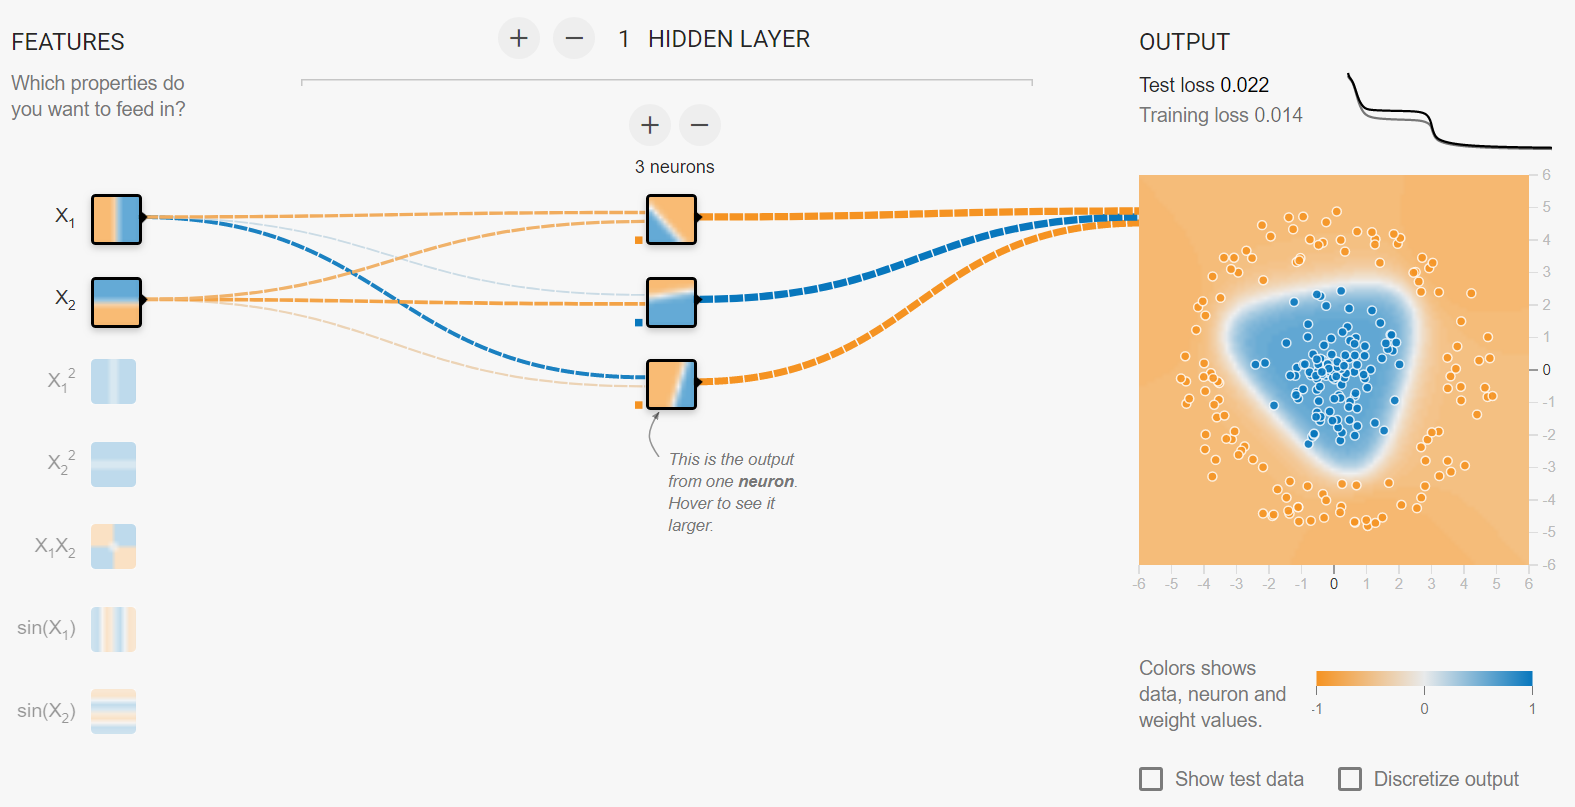
\includegraphics[width=0.75\textwidth]{images/simple_neuronal_network}
					\caption[Simple neural network with one hidden layer]{Simple neural network with one hidden layer\footnotemark}
					\label{fig:simple_neural_network}
				\end{figure}
				\footnotetext{Source: \url{http://playground.tensorflow.org/}}
		
			\subsubsection{Convolutional neural network}
			\label{sec:section_convolutional_neural_network}
				\de{Ein neuronales Netzwerk verarbeitet einen Vektor und gibt einen neuen Vektor zurück. Das Problem bei Eingabedaten wie Bildern ist, dass sie auf den ersten Blick nicht erfolgreich als Vektor beschrieben werden können, um mit einem normalem neuronalem Netzwerk trainiert werden zu können. Man braucht einen Algorithmus, welcher auch matrizenähnliche Eingaben verarbeiten kann und in der Lage ist Muster zu erkennen. Dabei wurde in der Vergangenheit das Prinzip der Convolutional Layer entwickelt. Ein Convolutional Layer nimmt ein Matrix Eingang entgegen, transformiert diese und gibt wie auch bei den künstlichen Neuronen einen Ausgangswert zurück (in diesem Fall eine weitere Matrix). Dieser Ausgangswert wird danach an die nächste Schicht weitergegeben. Dabei beinhaltet ein Convolutional Layer eine Menge \(n\) an quadratischen Matrizen (meist 3x3 oder 5x5 Matrizen). Diese Matrizen werden Filter genannt. Jeder Filter\footnote{Filter, welche z.B. Kanten, Ecken, Quadrate, etc. erkennen können und in tieferen Layern Dinge wie Augen, Ohren, Haare, etc.} wird nun jeweils von links oben bis rechts unten über die Pixel des Bildes mittels Skalarprodukt miteinander verrechnet, wobei ein neues Bild entsteht. Die soganannte Feature Map. Bei einer Anzahl von \(n\) Filtern entstehen am Ende \(n\) Feature Maps und heben die in den Filtern definierten Merkmale jeweils im neu errechneten Bild hervor (Figure \ref{fig:simple-convolution-and-simple-pooling}a). Dieser Vorgang wird auch Faltung genannt\autocite{deeplizard2017CNNExplained}.}
				\en{An \acl{ann} processes a vector and returns a new vector. The problem with input data such as images is that at first view they cannot be successfully described as vectors to be trained with a normal neural network. One needs an algorithm that can handle matrix-like inputs and that is able to recognize patterns. In the past the principle of the convolutional layer was developed. A convolutional layer receives a matrix input, transforms it and returns an output value (in this case another matrix). This output value is then passed on to the next layer. A convolutional layer contains a set \(n\) of square matrices (usually 3x3 or 5x5 matrices). These matrices are called filters. Each filter\footnote{Filters, which can recognize edges, corners, squares, etc. and in deeper layers things like eyes, ears, hair, etc.} is now calculated from top left to bottom right over the pixels of the image using a scalar product, which creates a new image (Figure \ref{fig:simple-convolution-and-simple-pooling}a). The so-called feature map. With a number of \(n\) filters, \(n\) feature maps are created at the end and highlight the features defined in the filters in the newly calculated image. This process is also called convolution\autocite{deeplizard2017CNNExplained}.}
				
				\begin{figure}[H]
					\centering
					\begin{tabular}{ ccccccc }
						image matrix (a) & & filter matrix (a) & & output matrix (a)(b) & & pooling (b) \\
					
						\begin{tabular}{|c|c|c|c|c|c|}
							\hline
							\tikzmark{tl11}0 & 1 & 1 & 0 & 1 & 1\\
							\hline
							1 & 1 & 1 & 0 & 1 & 0\\
							\hline
							0 & 1 & \tikzmark{tl21}0\tikzmark{br11} & 1 & 0 & 1\\
							\hline
							0 & 0 & 1 & 0 & 0 & 0\\
							\hline
							0 & 0 & 0 & 0 & 0\tikzmark{br21} & 1\\
							\hline
							0 & 0 & 1 & 0 & 0 & 0\\
							\hline
						\end{tabular} &
					
						\circled{$\times$} &
						\begin{tabular}{|c|c|c|}
							\hline
							1 & 1 & 1\\
							\hline
							1 & 1 & 0\\
							\hline
							0 & 0 & 1\\
							\hline
						\end{tabular} &
					
						\LARGE{$\rightarrow$} &
					
						\begin{tabular}{|c|c|c|c|}
							\hline
							\tikzmark{tl12}4\tikzmark{br12} & 5 & \tikzmark{tl31}3 & 4\\
							\hline
							5 & 3 & 3 & 2\tikzmark{br31}\\
							\hline
							1 & 3 & \tikzmark{tl22}2\tikzmark{br22} & 3\\
							\hline
							2 & 1 & 1 & 0\\
							\hline
						\end{tabular} &
						
						\LARGE{$\rightarrow$} &
						\begin{tabular}{|c|c|c|}
							\hline
							5 & \tikzmark{tl32}4\tikzmark{br32}\\
							\hline
							3 & 3\\
							\hline
						\end{tabular}
					\end{tabular}
					
					\DrawBox[thick, red]{tl11}{br11}
					\DrawBox[thick, red]{tl12}{br12}
					\DrawBox[thick, blue]{tl21}{br21}
					\DrawBox[thick, blue]{tl22}{br22}
					
					\DrawBox[thick, black!30!green, densely dotted, fill=green!50!white, fill opacity=0.2]{tl31}{br31}
					\DrawBox[thick, black!30!green, densely dotted, fill=green!50!white, fill opacity=0.2]{tl32}{br32}
					
					\vspace*{-10pt}
					\caption[Simple convolution and simple pooling]{Simple convolution and simple pooling}
					\label{fig:simple-convolution-and-simple-pooling}
				\end{figure}

				\de{Neuronale Netze, welche Gebrauch von Convolutional Layern machen, werden \acsp{cnn} und haben einen entscheidenden Beitrag zum Fortschritt der Bildklassifizierung und auch in anderen Bereichen wie Spracherkennung geleistet. Neben den Convolutional Layern existieren in einem Convolutional Neuronal Network weitere spezielle Layer, welche sich von normalen Neuronalen Netzen unterscheiden: Z.B. die Pooling Layer. In einem Pooling Layer werden überflüssige Informationen verworfen und die Featuremaps verkleinert (Figure \ref{fig:simple-convolution-and-simple-pooling}b). Dieser Vorgang verringert den Speicherbedarf und erhöht Berechnungsgeschwindigkeit. Die Convolutional Layer und die Pooling Layer wechseln sich in aller Regel jeweils ab, bis am Ende statt einer \(n x n\) Matrix des Eingangsbildes ein großer Vektor entsteht, welcher von einem normalen neuronalem Netzwerk weiterverarbeitet werden kann und schlußendlich in dem schon beschriebenen One Hot Vektor endet (Figure \ref{fig:traditional-convolutional-network}).}
				\en{Neural networks that make use of convolutional layers are called \acfp{cnn} and have made a decisive contribution to the progress of image classification and also in other areas like speech recognition. In addition to the convolutional layers, a \ac{cnn} has other special layers that differ from normal neural networks: For example the pooling layer. In a pooling layer, unnecessary information is discarded and feature maps are reduced in size (Figure \ref{fig:simple-convolution-and-simple-pooling}b). This process reduces memory requirements and increases calculation speed. The convolutional layer and the pooling layer usually alternate until a large vector is created at the end instead of a \(n x n\) matrix of the input image. This can be further processed by a normal neural network and finally ends in the already described one hot vector (Figure \ref{fig:traditional-convolutional-network}).}

				\begin{figure}[H]
					\centering
					\begin{tikzpicture}
						\tikzmath{
							\inputImageWidth = 1.0;
							\layerOneDistance = 0.22;
							\layerOnePosition = 1.95;
							\layerOneWidth = 1.0;
							\layerTwoDistance = 0.12;
							\layerTwoPosition = 4.40;
							\layerTwoWidth = 0.6;
							\layerThreeDistance = 0.12;
							\layerThreePosition = 6.50;
							\layerThreeWidth = 0.6;
							\layerFourDistance = 0.052;
							\layerFourPosition = 8.5;
							\layerFourWidth = 0.36;
						}

						\node[anchor=south west,inner sep=0,framed] (burger) at (0,0)
							{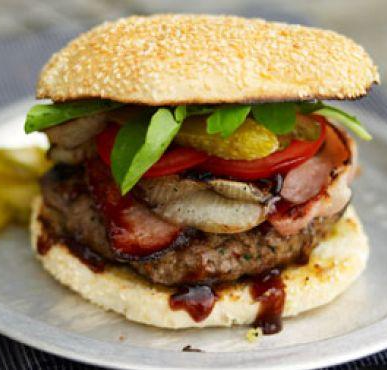
\includegraphics[width=6.5ex]{images/data/burger/burger28-quad.png}};

						% input image
						\node at (0.5,-1){\begin{tabular}{c}input image\end{tabular}};
						%\draw[opacity=1, draw=black]
						%	(0 * \inputImageWidth, 0 * \inputImageWidth) --
						%	(1 * \inputImageWidth, 0 * \inputImageWidth) --
						%	(1 * \inputImageWidth, 1 * \inputImageWidth) --
						%	(0 * \inputImageWidth, 1 * \inputImageWidth) --
						%	(0 * \inputImageWidth, 0 * \inputImageWidth);
						
						% layer 1
						\node at (3.0, 3.0){\begin{tabular}{c}convolutional layer\\layer $l = 1$\end{tabular}};
						\foreach \i in {5,...,0}
							\draw[fill=gray, opacity=0.8, draw=black]
								(\layerOnePosition + 0 * \layerOneWidth + \layerOneDistance*\i, 0 * \layerOneWidth + \layerOneDistance*\i) --
								(\layerOnePosition + 1 * \layerOneWidth + \layerOneDistance*\i, 0 * \layerOneWidth + \layerOneDistance*\i) --
								(\layerOnePosition + 1 * \layerOneWidth + \layerOneDistance*\i, 1 * \layerOneWidth + \layerOneDistance*\i) --
								(\layerOnePosition + 0 * \layerOneWidth + \layerOneDistance*\i, 1 * \layerOneWidth + \layerOneDistance*\i) --
								(\layerOnePosition + 0 * \layerOneWidth + \layerOneDistance*\i, 0 * \layerOneWidth + \layerOneDistance*\i);

						% layer 2
						\node at (5.0,-1){\begin{tabular}{c}pooling layer\\layer $l = 2$\end{tabular}};
						\foreach \i in {5,...,0}
							\draw[fill=gray, opacity=0.8, draw=black]
								(\layerTwoPosition + 0 * \layerTwoWidth + \layerTwoDistance*\i, 0 * \layerTwoWidth + \layerTwoDistance*\i) --
								(\layerTwoPosition + 1 * \layerTwoWidth + \layerTwoDistance*\i, 0 * \layerTwoWidth + \layerTwoDistance*\i) --
								(\layerTwoPosition + 1 * \layerTwoWidth + \layerTwoDistance*\i, 1 * \layerTwoWidth + \layerTwoDistance*\i) --
								(\layerTwoPosition + 0 * \layerTwoWidth + \layerTwoDistance*\i, 1 * \layerTwoWidth + \layerTwoDistance*\i) --
								(\layerTwoPosition + 0 * \layerTwoWidth + \layerTwoDistance*\i, 0 * \layerTwoWidth + \layerTwoDistance*\i);
						
						%layer 3
						\node at (7.5,3.0){\begin{tabular}{c}convolutional layer\\layer $l = 3$\end{tabular}};
						\foreach \i in {11,...,0}
							\draw[fill=gray, opacity=0.8, draw=black]
								(\layerThreePosition + 0 * \layerThreeWidth + \layerThreeDistance*\i, 0 * \layerThreeWidth + \layerThreeDistance*\i) --
								(\layerThreePosition + 1 * \layerThreeWidth + \layerThreeDistance*\i, 0 * \layerThreeWidth + \layerThreeDistance*\i) --
								(\layerThreePosition + 1 * \layerThreeWidth + \layerThreeDistance*\i, 1 * \layerThreeWidth + \layerThreeDistance*\i) --
								(\layerThreePosition + 0 * \layerThreeWidth + \layerThreeDistance*\i, 1 * \layerThreeWidth + \layerThreeDistance*\i) --
								(\layerThreePosition + 0 * \layerThreeWidth + \layerThreeDistance*\i, 0 * \layerThreeWidth + \layerThreeDistance*\i);
						
						% layer 4
						\node at (9.0,-1){\begin{tabular}{c}pooling layer\\layer $l = 4$\end{tabular}};
						\foreach \i in {11,...,0}
							\draw[fill=gray, opacity=0.8, draw=black]
								(\layerFourPosition + 0 * \layerFourWidth + \layerFourDistance*\i, 0 * \layerFourWidth + \layerFourDistance*\i) --
								(\layerFourPosition + 1 * \layerFourWidth + \layerFourDistance*\i, 0 * \layerFourWidth + \layerFourDistance*\i) --
								(\layerFourPosition + 1 * \layerFourWidth + \layerFourDistance*\i, 1 * \layerFourWidth + \layerFourDistance*\i) --
								(\layerFourPosition + 0 * \layerFourWidth + \layerFourDistance*\i, 1 * \layerFourWidth + \layerFourDistance*\i) --
								(\layerFourPosition + 0 * \layerFourWidth + \layerFourDistance*\i, 0 * \layerFourWidth + \layerFourDistance*\i);
						
						% layer 5
						\node at (12,3.0){\begin{tabular}{c}fully connected layer\\layer $l = 5$\end{tabular}};
						\draw[fill=teal,draw=black,opacity=0.8]
							(10.5,0) --
							(11,0) --
							(12.75,1.75) --
							(12.25,1.75) --
							(10.5,0);
						
						% layer 6
						\node at (13,-1){\begin{tabular}{c}fully connected layer\\output layer $l = 6$\end{tabular}};
						\draw[fill=teal,draw=black,opacity=0.8]
							(12.5,0.5) --
							(13,0.5) --
							(13.65,1.15) --
							(13.15,1.15) --
							(12.5,0.5);
					\end{tikzpicture}
					\caption[Architecture of a traditional convolutional neural network]{Architecture of a traditional convolutional neural network}
					\label{fig:traditional-convolutional-network}
				\end{figure}

				\de{Ein großer Vorteil von Convolutional neuronal networks soll nicht unerwähnt bleiben: Sie benötigen relativ wenig Vorverarbeitung im Vergleich zu anderen Bildklassifikationsalgorithmen. Dies bedeutet, dass das Netzwerk eigenständig die Filter lernt, die in herkömmlichen Algorithmen normalerweise von Hand entwickelt werden, wenn es mit ausreichender Schulung trainiert wird. Diese Eigenschaft dieser Netzwerke ist von großem Vorteil, da sie automatisiert durchgeführt werden können und sich bei Änderungen der Eingabedaten selbstständig ändern und keinem menschlichem Eingriff bedarf.}
				\en{A big advantage of convolutional neural networks should not remain unmentioned: They require relatively little preprocessing compared to other image classification algorithms. This means that the network independently learns the filters that are normally developed by hand in conventional algorithms, if trained with adequate training. This property of these networks is a great advantage because they can be automated and change independently when the input data changes and do not require human intervention.}
	
			\subsubsection{Transfer learning}
			\label{sec:section_transfer_learning}
				\de{\acp{cnn} sind großartig und haben einen entscheidenden Beitrag zur Klassifizierung von Bilder beigetragen. Mit der Gründung der Forschungsdatenbank ImageNet im Jahre 2006 werden jährliche Wettbewerbe veranstaltet, um entwickelte Neuronale Netzwerke miteinander zu vergleichen. ImageNet ist eine Bilderdatenbank mit mehr als 14 Millionen Bildern. Ein \ac{cnn} namens AlexNet im Jahr 2012 einen Top-5 Fehler von 15,3\% und erhöht sich aktuell stetig jedes Jahr. Aber die Architektur von einem \ac{cnn} hat ein Problem. Alle Convolutional Layer sind vom Beginn an zufällig initialisiert und enthalten noch keine Muster. Damit sie zuverlässig funktioniert, muss sie mit vielen Bildern trainiert werden. Würde man vom Scratch an ein \ac{cnn} selbst entwickeln und verwenden, so müssen alle Convolutional Layer auch vorab trainiert werden.}
				\en{\acp{cnn} are great and have made a significant contribution to the classification of images. With the foundation of the research database ImageNet in 2006, annual competitions are organized to compare developed neural networks. ImageNet is an image database with more than 14 million images. A CNN called AlexNet in 2012 got a top-5 error of 15.3\% and is currently increasing steadily every year. But the architecture of a \ac{cnn} has a problem. All convolutional layers are randomly initialized from the beginning and do not yet contain any patterns. For it to work reliably, it needs to be trained with many images. If one would develop and use a \ac{cnn} from scratch, all convolutional layers have to be trained in advance.}

				\de{Die Convolutional Layer extrahieren Features wie Kanten, Quadrate, Kreise, etc. Diese sind so gut wie in jedem Bild vorhanden und es stellt sich die Frage, ob man diese nicht wiederverwenden kann, um den Trainingsaufwand zu verringern. Die Idee beim Transfer Learning ist es ein schon vortrainiertes \ac{cnn} zu verwenden und lediglich das neuronale Netzwerk am Ende des Convolutional neuronal networks an die eigene Problemstellung anzupassen (Abbildung \ref{fig:transfer-learning-example}).}
				\en{The convolutional layers extract features such as edges, squares, circles, etc. These are present in almost every image and the question arises whether one can reuse them to reduce the training effort. The idea of \acl{tl} is to use an already pre-trained \ac{cnn} and just adapt the neural network at the end of the \acl{cnn} to the own problem (Figure \ref{fig:transfer-learning-example}).}

				\begin{figure}[H]
					\centering
					\begin{tikzpicture}
						\tikzmath{
							\inputImageWidth = 1.0;
							\layerOneDistance = 0.22;
							\layerOnePosition = 1.95;
							\layerOneWidth = 1.0;
							\layerTwoDistance = 0.12;
							\layerTwoPosition = 4.40;
							\layerTwoWidth = 0.6;
							\layerThreeDistance = 0.12;
							\layerThreePosition = 6.50;
							\layerThreeWidth = 0.6;
							\layerFourDistance = 0.052;
							\layerFourPosition = 8.5;
							\layerFourWidth = 0.36;
						}

						% placeholder
						\draw[fill=white, opacity=0, draw=white]
							(0 * \inputImageWidth, 0 * \inputImageWidth + .5) --
							(1 * \inputImageWidth, 0 * \inputImageWidth + .5) --
							(1 * \inputImageWidth, 1 * \inputImageWidth + .5) --
							(0 * \inputImageWidth, 1 * \inputImageWidth + .5) --
							(0 * \inputImageWidth, 0 * \inputImageWidth + .5);
						\draw[fill=white, opacity=0, draw=white]
							(0 * \inputImageWidth, 0 * \inputImageWidth - .5) --
							(1 * \inputImageWidth, 0 * \inputImageWidth - .5) --
							(1 * \inputImageWidth, 1 * \inputImageWidth - .5) --
							(0 * \inputImageWidth, 1 * \inputImageWidth - .5) --
							(0 * \inputImageWidth, 0 * \inputImageWidth - .5);

						%draw image
						%\node at (0.5,-1){\begin{tabular}{c}input image\end{tabular}};
						\node[anchor=south west,inner sep=0] (burger) at (0,0)
							{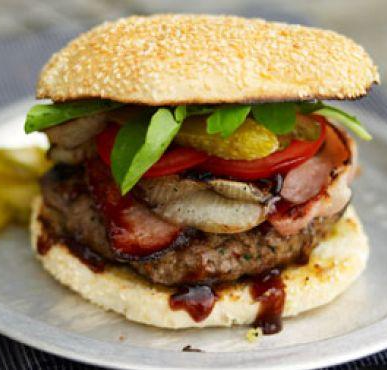
\includegraphics[width=6.5ex]{images/data/burger/burger28-quad.png}};

						% input image
						%\draw[fill=white, opacity=1, draw=black]
						%	(0 * \inputImageWidth, 0 * \inputImageWidth) --
						%	(1 * \inputImageWidth, 0 * \inputImageWidth) --
						%	(1 * \inputImageWidth, 1 * \inputImageWidth) --
						%	(0 * \inputImageWidth, 1 * \inputImageWidth) --
						%	(0 * \inputImageWidth, 0 * \inputImageWidth);
						
						% layer 1
						\foreach \i in {5,...,0}
							\draw[fill=gray, opacity=0.8, draw=black]
								(\layerOnePosition + 0 * \layerOneWidth + \layerOneDistance*\i, 0 * \layerOneWidth + \layerOneDistance*\i) --
								(\layerOnePosition + 1 * \layerOneWidth + \layerOneDistance*\i, 0 * \layerOneWidth + \layerOneDistance*\i) --
								(\layerOnePosition + 1 * \layerOneWidth + \layerOneDistance*\i, 1 * \layerOneWidth + \layerOneDistance*\i) --
								(\layerOnePosition + 0 * \layerOneWidth + \layerOneDistance*\i, 1 * \layerOneWidth + \layerOneDistance*\i) --
								(\layerOnePosition + 0 * \layerOneWidth + \layerOneDistance*\i, 0 * \layerOneWidth + \layerOneDistance*\i);

						% layer 2
						\foreach \i in {5,...,0}
							\draw[fill=gray, opacity=0.8, draw=black]
								(\layerTwoPosition + 0 * \layerTwoWidth + \layerTwoDistance*\i, 0 * \layerTwoWidth + \layerTwoDistance*\i) --
								(\layerTwoPosition + 1 * \layerTwoWidth + \layerTwoDistance*\i, 0 * \layerTwoWidth + \layerTwoDistance*\i) --
								(\layerTwoPosition + 1 * \layerTwoWidth + \layerTwoDistance*\i, 1 * \layerTwoWidth + \layerTwoDistance*\i) --
								(\layerTwoPosition + 0 * \layerTwoWidth + \layerTwoDistance*\i, 1 * \layerTwoWidth + \layerTwoDistance*\i) --
								(\layerTwoPosition + 0 * \layerTwoWidth + \layerTwoDistance*\i, 0 * \layerTwoWidth + \layerTwoDistance*\i);
						
						%layer 3
						\foreach \i in {11,...,0}
							\draw[fill=gray, opacity=0.8, draw=black]
								(\layerThreePosition + 0 * \layerThreeWidth + \layerThreeDistance*\i, 0 * \layerThreeWidth + \layerThreeDistance*\i) --
								(\layerThreePosition + 1 * \layerThreeWidth + \layerThreeDistance*\i, 0 * \layerThreeWidth + \layerThreeDistance*\i) --
								(\layerThreePosition + 1 * \layerThreeWidth + \layerThreeDistance*\i, 1 * \layerThreeWidth + \layerThreeDistance*\i) --
								(\layerThreePosition + 0 * \layerThreeWidth + \layerThreeDistance*\i, 1 * \layerThreeWidth + \layerThreeDistance*\i) --
								(\layerThreePosition + 0 * \layerThreeWidth + \layerThreeDistance*\i, 0 * \layerThreeWidth + \layerThreeDistance*\i);
						
						% layer 4
						\foreach \i in {11,...,0}
							\draw[fill=gray, opacity=0.8, draw=black]
								(\layerFourPosition + 0 * \layerFourWidth + \layerFourDistance*\i, 0 * \layerFourWidth + \layerFourDistance*\i) --
								(\layerFourPosition + 1 * \layerFourWidth + \layerFourDistance*\i, 0 * \layerFourWidth + \layerFourDistance*\i) --
								(\layerFourPosition + 1 * \layerFourWidth + \layerFourDistance*\i, 1 * \layerFourWidth + \layerFourDistance*\i) --
								(\layerFourPosition + 0 * \layerFourWidth + \layerFourDistance*\i, 1 * \layerFourWidth + \layerFourDistance*\i) --
								(\layerFourPosition + 0 * \layerFourWidth + \layerFourDistance*\i, 0 * \layerFourWidth + \layerFourDistance*\i);
						
						% layer 5
						\draw[fill=red,draw=black,opacity=0.8]
							(10.5,0) --
							(11,0) --
							(12.75,1.75) --
							(12.25,1.75) --
							(10.5,0);
						
						% layer 6
						\draw[fill=red,draw=black,opacity=0.8]
							(12.5,0.5) --
							(13,0.5) --
							(13.65,1.15) --
							(13.15,1.15) --
							(12.5,0.5);
					\end{tikzpicture}
					\caption[Architecture of a traditional \acl{cnn} with \ac{tl}]{The green area (see Figure \ref{fig:traditional-convolutional-network}) was replaced by a new \acl{nn} (red) adapted to the new problem.}
					\label{fig:transfer-learning-example}
				\end{figure}

				\de{Welchen Vorteil ein vortrainiertes Netzwerk hat, kann man in dieser Arbeit im Kapitel ``\nameref{sec:section_use_of_the_transfer_learning_approach}" einsehen.}
				\en{The advantage of a pre-trained network can be seen in the chapter ``\nameref{sec:section_use_of_the_transfer_learning_approach}" of this thesis.}
			
			\subsubsection{Overview of current and known convolutional neural networks}
				\de{Zu guter Letzt folgen hier noch ein paar aktuelle und bekannte Convolutional Neuronal networks. Sie unterscheiden sich hauptsächlich in folgenden Metriken, wobei in Kombination jedes Netzwerk seine Vor- und Nachteile besitzt:}
				\en{In the following a few current and well-known convolutional neural networks will be presented (Figure \ref{fig:comparison_cnn}). They differ mainly in the following metrics, whereby in combination each network has its advantages and disadvantages:}

				\begin{itemize}
					\setlength\itemsep{0em}
					\item the top-1 accuracy (based on the ImageNet image dataset)
					\item the computing operations which are required for a single forward pass (G-Ops)
					\item the model size (for comparison: the model size of \texttt{InceptionV3} is about 180 Mbyte)
				\end{itemize}
		
				\begin{figure}[H]
					\centering
					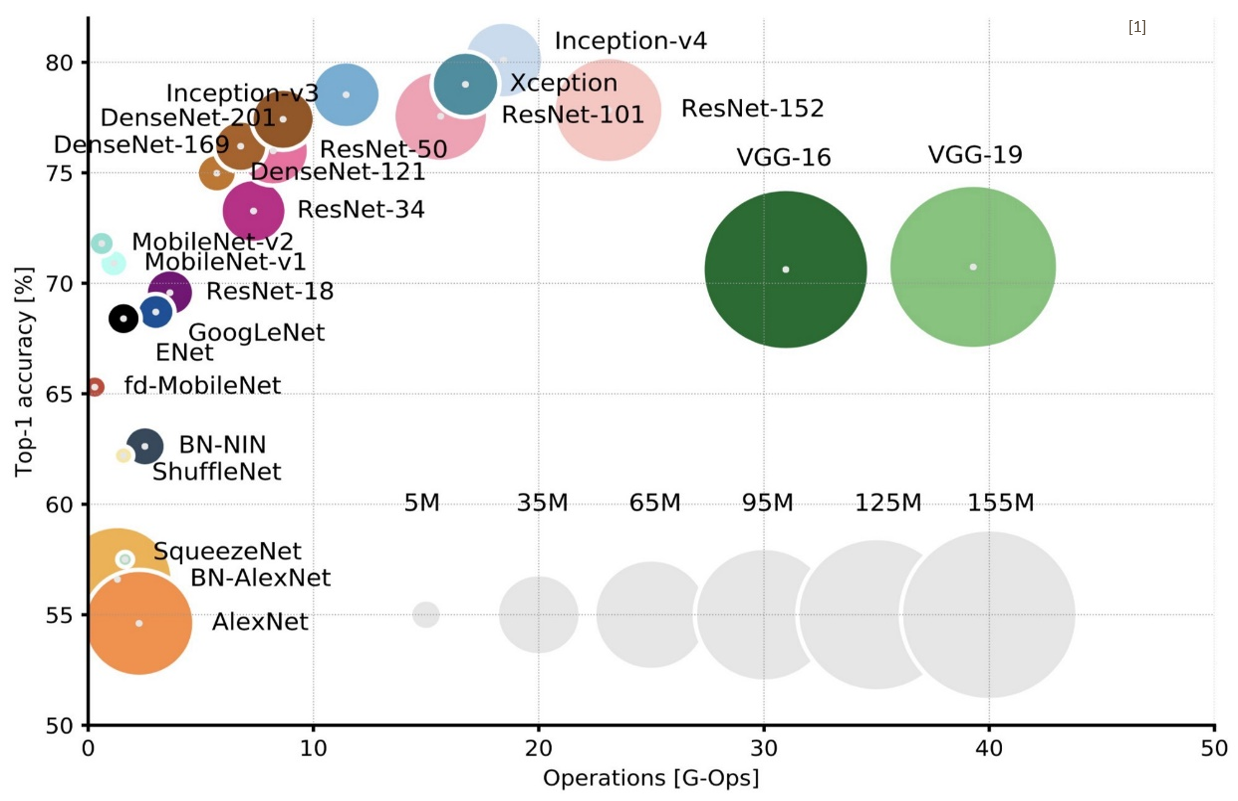
\includegraphics[width=0.75\textwidth]{images/tl_models}
					\caption[Overview of current and known convolutional neural networks]{Overview of current and known convolutional neural networks\footnotemark}
					\label{fig:comparison_cnn}
				\end{figure}
				\footnotetext{Source: \url{https://towardsdatascience.com/neural-network-architectures-156e5bad51ba}}



	% -------------------- %
	% Related work %
	% -------------------- %
	\pagebreak
	\section{Related work}
		\de{Es existieren eine Reihe von Untersuchungen zur Bildklassifikation auf sehr großen Datensätzen.\autocite{deng2010does}\textsuperscript{,}\autocite{sun2014deep}\textsuperscript{,}\autocite{krizhevsky2012imagenet} Meist ist diese riese Anzahl von Klassifikationsklassen und Datenmengen gar nicht erwünscht. Weiterhin gibt es viele Untersuchungen auf kleinen Datensätzen.\autocite{chollet2016building}\textsuperscript{,}\autocite{sagar_deep_2019} Was diesen Untersuchungen meist mangelt ist eine Übersicht und ein Vergleich der gängigen Hyperparameter in Bezug auf die Modellgenauigkeit in einer einzigen Arbeit. Diese Arbeit wird darauf eingehen. Daten sind teuer in der Beschaffung und meist nicht einfach zu bekommen (siehe Kapitel ``\nameref{sec:section_balanced_training_data_set}''). Und im Gegensatz dazu, treten Bildklassifikationen in immer mehr Bereichen unseres Lebens auf und finden auch in immer mehr in Unternehmen eine direkte Verwendung, welche bisher keinen Gebrauch davon gemacht haben und sich nun überlegen eigene Implemantionen einzuführen. Da sind z.B. Unternehmen, welche versuchen aufgrund verschiedener Daten Produkte zu klassifizieren. Ist es unter dem Kostenpunkte betrachtet eine gute Idee oder bleibt einem der Schritt zu den Softwaretools von Unternehmensriesen wie Microsoft, Google und Co. nicht verwehrt? Ein Mensch sieht ein Produkt  \(X\) und ordnet es ein: Anhand des Textes, der Beschreibungung oder eines Bildes. Manchmal bleibt nur noch ein Bild, weil z.B. Texte nicht richtig gepflegt wurden oder nur kryptische Werte zurückliefern. Und auch dann ist diese Klassifizierung für den Menschen oftmals keine Herausforderung, denn er erkennt auch in diesem Fall das Produkt \(X\) aufgrund des noch vorhandenen Bildes.}
		\en{There are a number of studies on image classification on very large datasets.\autocite{deng2010does}\textsuperscript{,}\autocite{sun2014deep}\textsuperscript{,}\autocite{krizhevsky2012imagenet} Most of the time this huge number of classification classes and datasets is not desired. Furthermore, there are many investigations on small data sets.\autocite{chollet2016building}\textsuperscript{,}\autocite{sagar_deep_2019} What these investigations usually lack is an overview and comparison of the common hyperparameters with respect to model accuracy in a single thesis. This thesis will deal with this. Data is expensive to obtain and usually not easy to get (see chapter ``\nameref{sec:section_balanced_training_data_set}''). And in contrast, image classifications are appearing in more and more areas of our life and are also being used directly in more and more companies that have not made use of them so far and are now considering introducing their own implementations. There are e.g. companies which try to classify products based on different data. Is it a good idea to implement your own implementation or is the step to the software tools of company giants like Microsoft, Google and Co. unavoidable? A person sees a product  \(X\) and classifies it: From the text, the description or an image. Sometimes only an image remains, because e.g. texts have not been maintained properly or only return cryptic values. And even then, this classification is often not a challenge for humans: Because in this case, they recognize the product \(X\) based on the still existing image.}
			
		
		
	% -------------------- %
	% Considerations and implementation %
	% -------------------- %
	\pagebreak
	\section{Considerations and implemention}
	\label{sec:section_considerations_and_implementation}
	
		\subsection{Research questions and hypthesis section}
			\de{Diese Arbeit beschäftigt sich mit dem Bildklassifizierungsteil. Zum Beispiel in der Anwendung für Unternehmen oder Umgebungen mit begrenzten Ressourcen. Folgende Fragen ergeben sich: Mit welchen Mitteln, Techniken und Ideen ist es möglich auch mit wenig Ressourcen ein erfolgreiches Bildklassifizierungsmodell zu erstelle? Müssen die in \fullref{sec:section_insufficient_amount_of_data} erwähnten Bedingungen erfüllt werden oder sind erfolgreiche Klassifizierungen auch schon mit weniger möglich? Kann man durch Anpassung bestimmter Abstimmungsparameter das Optimum aus der Erstellung von Modellen herausholen? Ist z.B. eine Clusteranalyse und die damit verbundene kategorische Untergliederung der Klassifizierung ein erfolgreicher Ansatz? Diese und andere Fragen sollen mit dieser Arbeit geklärt werden. Und ich wage an dieser Stelle zu behaupten, dass es möglich ist auch mit weniger Anforderungen zu einem guten Ziel zu kommen.}
			\en{This thesis deals with image classification applications with limited resources. The following questions arise: With which tools, techniques and ideas is it possible to create a successful image classification model even with few resources? Do the conditions mentioned in \fullref{sec:section_insufficient_amount_of_data} have to be fulfilled or are successful classifications already possible with less? Is it possible to get the most out of model creation by adjusting certain tuning parameters? For example, is a cluster analysis and the associated categorical breakdown of the classification a successful approach? The following chapters will show that it is possible to reach a good classification accuracy even with a small traning data set.}
	
		\subsection{Working environment and model creation}
			\de{Der gesamte Quellcode für die Umgebung und das Framework um Modelle trainieren zu können und welche für diese Arbeit verwendet worden sind, sind sind in einem Github-Repository öffentlich einsehbar\autocite{hempel_keras_2020}. Dieses Framework erlaubt es alle hier in der Arbeit genannten Hyperparameter einzustellen\autocite{hempel_keras_nodate}. Nachfolgend ein Beispiel für ein Kommandozeilenaufruf mit den Standardwerten aus dem Kapitel ``\nameref{sec:section_default_setup}'' (Listing \ref{lst:listing_command_call}). Das erstellte Modell befindet sich im angegebenen Verzeichnis mit dem Namen \texttt{model.h5}:}
			\en{All source code for the environment and the framework to train models and which has been used for this thesis is available in a GitHub repository\autocite{hempel_keras_2020}. This framework allows to set all the \aclp{hp} mentioned in this thesis\autocite{hempel_keras_nodate}. Below is an example of a command line call with the default values from the chapter ``\nameref{sec:section_default_setup}'' (Listing \ref{lst:listing_command_call}). The created model is located in the specified directory with the name \texttt{model.h5}:}

			\begin{lstlisting}[frame=single,caption={Example command line call to train the given data path},captionpos=b,basicstyle=\small,language=bash,label=lst:listing_command_call]
user$ ml train \
      --use-train-val \
      --data-path=./data/raw/food-50 \
      --model-file=./data/processed/experiment1/type-of-experiment/model.h5
			\end{lstlisting}
	
		\subsection{Performance}
		\label{sec:section_performance_gpu_cpu}
			\de{Wenn man beabsichtigt ein Deep Neuronal Networks (DNN) zu implementieren und zu optimieren, müssen die Berechnungen auf der GPU erfolgen. Es ist auch möglich, Berechnungen auf der \ac{cpu} durchzuführen. Auch die Installation von Keras für CPU-gesteuerte Berechnungen ist viel einfacher, da die Installation der GPU-Treiber nicht notwendig ist. Dies hat jedoch den Nachteil, dass das Training größerer Modelle wesentlich länger dauert. Gute Modelle für die Klassifizierung von z.B. Bildern werden erst nach mehreren Trainingseinheiten erreicht. Trainingseinheiten erfordern viel Rechenleistung in Form von vielen Matrixoperationen. Eine GPU ist prädestiniert für Matrixoperationen\autocite{fatahalian2004understanding}.}
			\en{If one intends to implement and optimize \acp{dnn}, the calculations must take place on the \ac{gpu}. It is also possible to run calculations on the \ac{cpu}. Also, the installation of Keras for \ac{cpu} driven computations is much easier, because the installation of the \ac{gpu} drivers is not necessary. The disadvantage of this, however, is that it takes much longer to train larger models. Good models for the classification of e.g. pictures are only achieved after several training units. Training units require a lot of computing power in the form of many matrix operations. A \ac{gpu} is predestined for matrix operations\autocite{fatahalian2004understanding}.}
			
			\de{Tabelle \ref{tbl:table_performance_comparison} im Anhang zeigt einen tabellarischen Leistungsvergleich auf der Grundlage des Kaggle-Blumendatensatzes Training\autocite{noauthor_flowers_nodate}. Dieser Bildersatz besteht aus 5 Klassen mit etwa 4242 Trainingsbildern (10 epochs, \texttt{InceptionV3})\autocite{hempel_keras_nodate-1} und wurde mit den Standard-Werten aus Kapitel ``\nameref{sec:section_default_setup}'' trainiert.}
			\en{Table \ref{tbl:table_performance_comparison} in the appendix in shows a tabular comparison of performance based on the Kaggle flower data set training\autocite{noauthor_flowers_nodate}. This image set consists of 5 classes with about 4242 training images\autocite{hempel_keras_nodate-1} and was trained with the default values from chapter ``\nameref{sec:section_default_setup}'' (but with only 10 epochs, \texttt{InceptionV3}).}
			
			\de{Während die Art des Rechengerätes (CPU or GPU) keinen Unterschied ausmacht was die Vor- und Nachbereitung betrifft, so macht es aber einen entscheidenden Unterschied bei der Trainingszeit. Die langsamste CPU benötigt mehr als 80 mal soviel Zeit, wie die schnellste Grafikkarteneinheit. Die Wahl des Rechengerätes für alle weiteren Tests fällt eindeutig auf die GPU, weshalb alle Experimente (wenn nicht anders angegeben) auf einer NVIDIA trainiert wurden.}
			\en{While the type of computing device (\ac{cpu} or \ac{gpu}) makes no difference in terms of preparation and postprocessing, it makes a significant difference in training time. The slowest \ac{cpu} takes more than 80 times as many time as the fastest graphics card unit. The choice of the computing device for all further tests clearly falls on the \ac{gpu}, so all experiments (unless otherwise specified) were trained on Nvidia GTX 1060 with 6 Gbyte of memory.}
	
		\subsection{Experimental Setup}
		\label{sec:section_experiment_setup}
		
			\subsubsection{Software specification}
			\label{sec:section_software_specifics}
				\paragraph*{Python v3.6.9}
					\de{Python ist in den letzten Jahren zu den wichtigsten Programmiersprachen im Bereich des Machine Learnings und der Datenwissenschaften herangewachsen.\autocite{noauthor_most_2015} Die Sprache wurde als Programmiersprache gewählt, da es eine große Anzahl von \ac{ml}-Bibliotheken zur Auswahl hat. Die Tatsache das die TensorFlow \ac{api} hauptsächlich auf die Verwendung mit Python ausgerichtet ist und damit eine stabile Entwicklung möglich ist, trug ebenfalls zur Wahl bei.}
					\en{Python has become one of the most important programming languages in the field of machine learning and data sciences in recent years.\autocite{noauthor_most_2015} The language was chosen as programming language because it has a large number of \ac{ml} libraries to choose from. The fact that the TensorFlow \ac{api} is mainly designed for use with Python and thus allows stable development is also a contributing factor to the choice.}
				
				\paragraph*{TensorFlow GPU v1.14.0 and Keras-GPU v2.2.4}
					\de{TensorFlow GPU wurde in Verbindung mit Keras-GPU v2.2.4 gewählt, um die Berechnungen auf der GPU und nicht auf der CPU durchzuführen. Dies hat die Zeit der Modellerstellung erheblich verkürzt (siehe Kapitel ``\nameref{sec:section_performance_gpu_cpu}'').}
					\en{TensorFlow GPU was chosen in conjunction with Keras GPU v2.2.4 to perform the calculations on the GPU and not on the CPU. This has significantly reduced the time of model creation (see chapter ``\nameref{sec:section_performance_gpu_cpu}'').}
				
				\paragraph*{Keras v2.2.4}
					\de{Bei den nachfolgenden Experimenten wird TensorFlow als Backend verwendet. Keras übersetzt die Funktionsaufrufe in die entsprechenden Funktionen von TensorFlow. Keras als als obergeordnete Bibliothek vereinfacht die Verwendung von Tensorflow, vereinfacht den Code, macht ihn lesbarer und minimiert Fehler.}
					\en{In the following experiments TensorFlow is used as backend. Keras translates the function calls into the corresponding functions of TensorFlow. Keras as the parent library simplifies the use of TensorFlow, makes the code easier to read and minimizes errors.}
				
				\begin{comment}
				\paragraph*{Deeplearning4j v1.0.0-beta3}
					\de{Deeplearning4j ist eine Programmierbibliothek für tiefes Lernen, die für Java geschrieben wurde, sowie ein Computerframework mit breiter Unterstützung für Algorithmen für tiefes Lernen\autocite{noauthor_deeplearning4j_2019}. Sie wird in dieser Arbeit nicht explizit für die Modellerstellung verwendet, jedoch sei erwähnt, dass man mit dieser Programmierbibliothek Keras-Modelle einlesen und verwenden kann\autocite{hempel_keras_2019}.}
					\en{Deeplearning4j is a deep learning programming library written for Java and a computer framework with wide support for deep learning algorithms\autocite{noauthor_deeplearning4j_2019}. It is not explicitly used for model creation in this thesis, but it should be mentioned that this programming library allows to read in and use Keras models\autocite{hempel_keras_2019}.}
				\end{comment}

			\subsubsection{Used data set}
			\label{sec:section_used_data_set}
				\de{Beim verwendeten Datensatz handelt es sich um einen Essensdatensatz bestehend aus 50 Klassen, 14.866 Bilddateien und hat eine Größe von 765 MB (\texttt{food-50}). Dieser Datensatz wurde händisch erstellt und gelabelt. Die Dateien sind ungleichmäßig zwischen den Klassen verteilt (unbalanced). Bevor man den Trainingsprozess beginnen kann, muss der verwendete Datensatz in einen Trainings- und einen Validierungsdatensatz aufgeteilt werden. Als Verhältnis wurden 80\% Trainings- und 20\% Validierungsdaten gewählt (11.913 Bilder versus 2,953 Bilder). Die Klasse mit dem kleinsten Bilderset ist \texttt{french\_fries} und enthält 36 Trainingsbilder und 8 Validierungsbilder. Die Klasse mit dem größten Bilderset ist \texttt{grilled\_cheese\_sandwich} und enthält über 390 Bilder im Trainingsdatensatz, sowie über 97 Bilder im Validierungsdatensatz. Im Schnitt enthalten alle Klassen rund 240 Trainingsdaten, sowie 60 Testdaten (im Detail in Abbildung \ref{fig:implementation_number_train_files} zu einzusehen). Ein Testdatensatz wird in dieser Arbeit nicht verwendet.}
				\en{The used data set is a food data set consisting of 50 classes, 14,866 image files and has a size of 765 Mbyte (\texttt{food-50}). This data set was created and labelled manually. The files are unevenly distributed between the classes (unbalanced). Before you can start the training process, the used data set must be split into a training and a validation data set.  As a ratio 80\% training and 20\% validation data was chosen (11,913 images versus 2,953 images). The class with the smallest image set is \texttt{french\_fries} and contains 36 training images and 8 validation images. The class with the largest image set is \texttt{grilled\_cheese\_sandwich} and contains over 390 images in the training data set and over 97 images in the validation data set. On average, all classes contain about 240 training data and 60 test data (see Figure \ref{fig:implementation_number_train_files} for details). A test data set is not used in this thesis.}

				\subsubsection{Default setup}
				\label{sec:section_default_setup}
					\de{Mit Ausnahme der \ac{cnn}-Modellversuche basierten alle Tests auf den folgenden Parametern (wobei ein Wert der Parameter je nach Kapitel variierte):}
					\en{With the exception of the \ac{cnn} model tests, all tests were based on the following parameters
				(whereby one value of the parameters varied depending on the chapter):}
			
					\begin{itemize}
						\setlength\itemsep{0em}
						\item \textbf{model:} \texttt{InceptionV3}
						\item \textbf{learning rate:} 0,001 (decreases every 7 epochs to 50\% of the previous value)
						\item \textbf{epochs:} 21 (the learning rate \(\eta\) from epoch 15 to 21 is 0.00025)
						\item \textbf{image size:} 299x299 pixels\footnote{The original image is reduced to 299 pixels. If it is not a square image, the larger side is scaled down to 299 pixels.}
						\item \textbf{batch size:} 16
						\item \textbf{drop out:} 50\%
						\item \textbf{\ac{cnn} weights:} ImageNet
						\item \textbf{activation function:} ReLU
						\item \textbf{optimizer:} \ac{sgd} with Nesterov
						\item \textbf{momentum:} 0.9 (with decay 0.0)
						\item the entire training and validation set (14,866 images - unless otherwise specified)
					\end{itemize}
					
				\de{\noindent Verschiedene Modelle wurden im Kapitel ``\nameref{sec:section_validation_compare_cnn_models}'' mit den gleichen Parametern wie oben ausprobiert: \texttt{DenseNet121}, \texttt{DenseNet201}, \texttt{InceptionResNetV2}, \texttt{InceptionV3}, \texttt{NASNetLarge}, \texttt{ResNet50}, \texttt{VGG19} und \texttt{Xception}}
				\en{\noindent Different models were tried out in chapter ``\nameref{sec:section_validation_comparison_cnn_models}'' with the same parameters as above: \texttt{DenseNet121}, \texttt{DenseNet201}, \texttt{InceptionResNetV2}, \texttt{InceptionV3}, \texttt{NASNetLarge}, \texttt{ResNet50}, \texttt{VGG19} and \texttt{Xception}}

	% -------------------- %
	% Results %
	% -------------------- %
	\pagebreak
	\section{Results}
	\label{sec:section_results}
		\de{In diesem Teil der Arbeit werden die Untersuchungen vorgestellt und die entsprechenden Auswertungen dazu. Dabei wurden in den jeweiligen Kapiteln Modelle mit den angegebenen Parametern und Techniken erstellt mit welcher man in der Lage ist Bildklassifikationen durchzuführen. Das Modell muss trainiert werden, wobei eine Entscheidung auf viele variable Parameter wie die Lernrate \(\eta\), die Optimierer, aber auch Dinge wie das \ac{cnn} Modell gefällt werden muss. Als Basis dient ein Standardsetup, welches Kapitel ``\nameref{sec:section_default_setup}'' erklärt wurde. Von diesem Standard-Setup ausgehend werden die variablen Parameter in den entsprechenden Kapiteln jeweils verändert und diskutiert. Das Ziel soll sein die Parameter zu finden, mit welchem die Erkennungsgenauigkeiten der Modelle besonders hoch ausfallen: hohe Genauigkeiten und kleiner Verlust (loss function).}
		\en{In this part of the thesis the investigations and the corresponding evaluations will be presented. For each chapter models with the given parameters and techniques have been created with which image classifications can be performed. The model has to be trained, whereby a decision has to be made on many variable parameters like the learning rate \(\eta\), the optimizers, but also things such as the \ac{cnn} model. The basis is a standard setup, which was explained in chapter ``\nameref{sec:section_default_setup}''. Starting from this standard setup, the variable parameters are changed and discussed in the corresponding chapters. The goal is to find the parameters with which the recognition accuracy of the models is particularly high: high accuracy and small loss function.}
	
		\subsection{Model validation}
		\label{sec:section_model_validation}

			\subsubsection{Influence of number of trained images on accuracy}
			\label{sec:section_validation_number_of_train_files}
	
				\de{Die erste Frage die sich stellt: Welchen Einfluß hat die Anzahl der zu trainierenden Daten auf die Genauigkeit des Modells? Hierzu wird das Standard-Setup aus dem Kapitel ``\nameref{sec:section_default_setup}'' verwendet und das Modell mit einer verschiedenen Anzahl von Trainingsdaten trainiert. Während das Validierungsdatenset immer gleich bleibt, wird die Gesamtanzahl der zu trainierenden Daten von 500 stückweise auf die Gesamtanzahl von 11.913 erhöht. Da es sich um einen unausgeglichenen Datensatz handelt, bleibt prozentuall gesehen die Anzahl in den jeweiligen Klassen gleich. Lediglich die Gesamtanzahl wird auf die entsprechenden Werte verändert: 500, 1.000, 2.000, etc.}
				\en{The first question that comes up: What influence does the amount of data to be trained have on the accuracy of the model? For this purpose, the standard setup from the chapter ``\nameref{sec:section_default_setup}'' is used and the model is trained with a different number of training data. While the validation data set always stays the same, the total number of data to be trained is increased from 500 data sets to the total number of 11,913. Since this is an unbalanced data set, the number remains the same in each class in percentage terms. Only the total number is changed to the corresponding values: 500, 1,000, 2,000, etc. (Figure \ref{fig:evaluation_number_train_files}).}
				
				\begin{figure}[H]
					\begin{center}
						\scalebox{1.0}{
							\inputpgf{images/evaluation}{number_train_files.pgf}
						}
					\end{center}
					\vspace*{-20pt}
					\caption{Overview of influence of number of trained images on accuracy}
					\label{fig:evaluation_number_train_files}
				\end{figure}

				\de{Wie erwartet hat die Anzahl der zu trainierenden Bilder einen entscheidenden Einfluß auf die Modellgenauigkeit. Während mit 500 Bildern eine Genauigkeit von 45,76\% erreicht werden kann, sind es mit fast 12.000 Bildern schon 83,59\% nach 21 Epochen. Mit jeder Erhöhung der Bildanzahl kann man eine Verbesserung der Genauigkeit feststellen. Der Anstieg der Genauigkeit erfolgt nicht linear mit Zunahme der Trainingsdatensätze. Obwohl die Genauigkeit im oberen Bereich (mehr als 8,000 Bilder) immer noch zu steigen scheint, so sind die Sprünge nicht mehr sehr groß und bewegen sich offenbar an eine Grenze. Für weitere Nachforschungen wäre es eine gute Idee, ab welcher Anzahl von Trainingsdatensätzen keine weiteren signifikanten Steigerungen in der Genauigkeiten mehr möglich sind. Da in diesem Datenset keine weiteren Daten mehr zur Verfügung standen, wird dieses Vorhaben hier nicht weiter verfolgt.}
				\en{As expected, the number of images to be trained has a significant influence on the model accuracy. While with 500 images an accuracy of 45.76\% can be achieved, with almost 12,000 images it is already 83.59\% after 21 epochs. With every increase in the number of images, an improvement in accuracy can be observed. The improvement in accuracy is not linear with an increase in training data sets. Although the accuracy in the upper range (more than 8,000 images) still seems to increase, the jumps are not very big anymore and seem to be moving to a limit. For further research, it would be a good idea to find out from which number of training data sets no further significant increases in accuracy are possible. Since no further data was available in this data set, this project will not be pursued further here.}
				
				\de{Ein weiterer interessanter Punkt ist die Tatsache, dass mit der Erhöhung der Trainingsdaten theoretisch bis zu einem gewissen Punkt Rechenzeit eingespart werden kann. Sind die Datensätze nämlich deutlich zu klein, so erreicht man während des Trainings niemals eine Genaugkeit, welche Modelle mit wesentlich mehr Daten schon mit der ersten Epoche erreichen und übersteigen. Deutlich zu sehen: Bei 1000 Bildern (orangene Linie) kommt man maximal auf eine Genauigkeit von 61,42\% nach 18 Epochen und ungefähr 20 Minuten Rechenzeit. Verwendet man die 10-fache Menge an Bildern (10000 Bilder - braune Linie), so erreicht man schon in der ersten Epoche nach sechseinhalb Minuten eine Genauigkeit von 68,1\%.}
				\en{Another interesting point is the fact that increasing the training data theoretically saves computing time up to a certain point. If the data sets are significantly too small, one will never reach an accuracy during training, which models with much more data reach and exceed already with the first epoch. Clearly to see: With 1,000 images (orange trace) one gets a maximum accuracy of 61.42\% after 18 epochs and about 20 minutes of computing time. If one uses 10 times the amount of images (10,000 images - brown trace), one reaches an accuracy of 68.1\% already in the first epoch after six and a half minutes.}

			\subsubsection{Comparison of different \ac{cnn} models}
			\label{sec:section_validation_comparison_cnn_models}
				\de{Derzeit gibt es viele \ac{cnn} Modelle und jedes Jahr mit dem alljährlichem ImageNet-Wettbewerb kommen neue Modelle mit besseren Genauigkeiten heraus. Diese Modelle werden trainiert mit dem ImageNet Dataset und die Ergebnisse anhand dieser Datenbasis verglichen. Wie sieht das Ergebnis mit kleineren Datensets aus? Das Trainingsergebnis nach dem Standard-Setup und mit jeweils unterschiedlichem \ac{cnn} Modell von acht Modellen sieht wie folgt aus:}
				\en{There are currently many \ac{cnn} models and each year with the annual ImageNet competition new models with better accuracy are released. These models are trained with the ImageNet dataset and the results are compared using this set of data. What is the result with smaller sets of data? The training result according to the standard setup and with different \ac{cnn} models of eight models is as follows (Figure \ref{fig:evaluation_different_models}).}

				\begin{figure}[H]
					\begin{center}
						\scalebox{1.0}{
							\inputpgf{images/evaluation}{different_models.pgf}
						}
					\end{center}
					\vspace*{-20pt}
					\caption{Overview of known \ac{cnn} models}
					\label{fig:evaluation_different_models}
				\end{figure}

				\de{Alle Modelle mit Ausnahme von \texttt{DenseNet201} und \texttt{NASNetLarge} wurden mit einer Batch Size von 16 trainiert (\(bs=16\)). Aufgrund des begrenzten Speichers von 6GB der Nvidia GTX 1060\footnote{GeForce 10 series, Wikipedia contributors, February 22, 2020, \url{https://en.wikipedia.org/wiki/GeForce_10_series}} wurden \texttt{DenseNet201} mit einer Batch Size von 8 und \texttt{NASNetLarge} mit einer Batch Size von 4 trainiert. Ein wirklicher Vergleich dieser beiden Ausnahmen ist somit nicht wirklich möglich, soll jedoch an dieser Stelle auch nicht weggelassen werden. Ein größerer Batch-Wert geht mit erhöhter Rechenzeit und langsameren Ansteigen von der Genauigkeit einher (siehe Kapitel ``\nameref{sec:section_validation_comparison_different_bs}''). Ein Vergleich mit Darstellung \fullref{fig:comparison_cnn} zeigt ähnliche Genauigkeiten und benötigte Rechenzeiten: Das beste Modell wurde mit \texttt{DenseNet201} mit einer Genauigkeit von 88,58\% erreicht. Das Modell mit der geringsten Genauigkeit ist das schon etwas ältere VGG19 Modell mit 77,29\%. Stellt man Rechenzeit und zu erreichende Genauigkeiten gegenüber, so fällt einem das \texttt{InceptionV3} Modell auf (rote Kurve). Es ist das zweitbeste Modell und erreicht das Ergebnis in einem mittlerem Bereich von ca. zweieinhalb Stunden. Das beste Modell \texttt{DenseNet201} benötigt für sein Ergebnis mehr als doppelt soviel Zeit. Die Wahl für alle weiteren Experimente viel aus diesem Grund auf das \ac{cnn} Modell \texttt{InceptionV3}, da es ein gutes Ergebnis innerhalb einer vergleichsweisen geringen Zeitspanne erreicht.}
				\en{All models except \texttt{DenseNet201} and \texttt{NASNetLarge} were trained with a batch size of 16 (\(bs=16\)). Due to the limited 6 Gbyte memory of the Nvidia GTX 1060\footnote{GeForce 10 series, Wikipedia contributors, February 22, 2020, \url{https://en.wikipedia.org/wiki/GeForce_10_series}}, \texttt{DenseNet201} was trained with a batch size of 8 and \texttt{NASNetLarge} with a batch size of 4. A real comparison of these two exceptions is not really possible, but should not be omitted at this point. A larger batch value is associated with increased computing time and slower increase in accuracy (see chapter ``\nameref{sec:section_validation_comparison_different_bs}''). A comparison with Figure \ref{fig:comparison_cnn} (``\nameref{fig:comparison_cnn}'') shows similar accuracies and required computing time: The best model was achieved with \texttt{DenseNet201} with an accuracy of 88.58\%. The model with the lowest accuracy is the somewhat older VGG19 model with 77.29\%. If one compares the computing time and the accuracies to be achieved, one notices the \texttt{InceptionV3} model (red trace). It is the second best model and reaches the result in a medium range of about two and a half hours. The best model \texttt{DenseNet201} needs more than twice as much time for its result. The choice for all further experiments is therefore the \ac{cnn} model \texttt{InceptionV3}, because it achieves a good result within a comparatively short period of time.}
		
			\subsubsection{Use of the \acf{tl} approach}
			\label{sec:section_use_of_the_transfer_learning_approach}
	
				\de{Welchen Einfluss auf die Genauigkeit hat das Verwenden von Transfer Learning? Wie im Kapitel ``\hyperref[sec:section_transfer_learning]{Transfer learning}'' beschrieben, verbessert der Transfer Learning Ansatz sofort die Genauigkeit, da das Modell schon Erkennungsmerkmale besitzt, welche ein ungelerntes Netzwerk erst noch lernen muss. Der Ansatz wird auf den Datensatz \texttt{food-50} angewendet. Weiterhin wird untersucht was passiert, wenn der Datensatz ohne \ac{tl} Ansatz statt der bisher verwendeten 21 Epochen mit 49 Epoche trainiert wird. Dabei wird ein Dropout von \(dropout=0.5\) aus dem Standard-Setup und ein Dropout von \(dropout=0.0\) verwendet um ein Overfitting zu erzwingen und die Konzentration auf das Erlernen der Erkennungsmerkmale zu legen:}
				\en{What influence does the use of transfer learning have on accuracy? As described in the chapter ``\hyperref[sec:section_transfer_learning]{Transfer learning}'', the \ac{tl} approach immediately improves accuracy because the model already has recognition features that an unlearned network has yet to learn. The approach is applied to the data set \texttt{food-50}. Furthermore, it is examined what happens if the data set without \ac{tl} approach is trained with 49 epochs instead of the 21 epochs used so far. A dropout of \(dropout=0.5\) from the default setup and a dropout of \(dropout=0.0\) is used to force overfitting and focus on learning the recognition features (Figure \ref{fig:evaluation_transfer_learning}).}
				
				\begin{figure}[H]
					\begin{center}
						\scalebox{1.0}{
							\inputpgf{images/evaluation}{transfer_learning.pgf}
						}
					\end{center}
					\vspace*{-20pt}
					\caption{Overview of use of the \ac{tl} approach}
					\label{fig:evaluation_transfer_learning}
				\end{figure}
				
				\begin{figure}[H]
					\begin{center}
						\scalebox{1.0}{
							\inputpgf{images/evaluation}{transfer_learning_without.pgf}
						}
					\end{center}
					\vspace*{-20pt}
					\caption{Overview of training without \ac{tl} approach}
					\label{fig:evaluation_transfer_learning_without}
				\end{figure}

				\de{Wie erwartet erziehlt das Modell mit dem Transfer Learning Ansatz ein besseres Ergebnis bei gleicher Rechenzeit (blaue Linie versus orangene Linie). In der ersten Epoche erreicht das Modell ohne Transfer Learning Ansatz einen Genauigkeitswert von 8,5\% und steigert sich in 21 Lernepochen auf 38,2\%. Die Trainingsgenauigkeit mit 58,8\% liegt dabei noch weit unter den Werten, welche mit TL nach wenigen Epochen erreicht werden. Dies bedeutet, das ein Lernen von Features mit den vorhandenen Daten weiter erfolgen kann. Beginnt man mit einem trainierten Netzwerk, so erreicht man schon mit der ersten Epoche einen besseren Genauigkeitswert von 68,9\% und kann diesen weiter steigern bis 83,6\% in der 21. Epoche. Die rote und grüne Linie verfolgen den Ansatz die Genauigkeit auch ohne TL weiter zu erhöhen. Dabei ließ sich vor allem mit einem Dropout von \(dropout=0.0\) eine Genauigkeit von 48,2\% erreichen (immer noch unter dem Wert mit TL Ansatz), wobei die Trainingsgenauigkeit schon bei 99,59\% angelangt ist. Damit ist ein weiteres Generalisieren theoretisch nicht mehr möglich. Um hier weitere Fortschritte zu erzielen und bessere Genauigkeiten auf bisher unbekannte Bilder zu erreichen, werden weitere Bilder zum Lernen von Featues benötigt. Fazit: Für das Trainieren von Ansätzen ohne TL reicht das aktuell vorhandene Bilderset nicht mehr aus um bessere oder gleiche Werte wie beim TL Ansatz zu erreichen. Transfer Learning zu verwenden ist gerade bei der Verwendung kleiner Datensätze eine gute Idee.}
				\en{As expected, the model with the \ac{tl} approach achieves a better result in the same computing time (blue trace versus orange trace). In the first epoch the model without transfer learning approach reaches an accuracy value of 8.5\% and increases to 38.2\% in 21 learning epochs. The training accuracy of 58.8\% is still far below the values achieved with \ac{tl} after a few epochs. This means that learning of features can be continued with the existing data set. If one starts with a pre-trained network, a better accuracy value of 68.9\% is achieved in the first epoch and can be further increased to 83.6\% in the 21st epoch. The red and green trace follow the approach to increase the accuracy even without \ac{tl}. Especially with a dropout of \(dropout=0.0\) an accuracy of 48.2\% could be achieved (still below the value with \ac{tl} approach), whereas the training accuracy has already reached 99.59\%. Thus, further generalization is theoretically no longer possible. In order to make further progress and to achieve better accuracies on previously unseen images, more images are needed to learn features. Conclusion: For the training of approaches without \ac{tl} the currently available image set is no longer sufficient to achieve better or the same values as with \ac{tl} approaches. Using transfer learning is a good idea especially when using small data sets.}
				
			\subsubsection{Influence of the number of trained layers on the accuracy}
				\de{Ein vortrainiertes Netzwerk hat einen entscheidenden Einfluss auf die zu erreichende Genauigkeit, die man in einer gewissen Rechenzeit erreichen kann. Mit fortschreitender Tiefe der Ebenen eines \ac{cnn} Modells, haben die dazugehörigen Filter mehr und mehr komplexere Erkennungsmerkmale gelernt\footnote{Advanced Topics in Deep Convolutional Neural Networks, https://towardsdatascience.com, February 22, 2020, \url{https://towardsdatascience.com/advanced-topics-in-deep-convolutional-neural-networks-71ef1190522d}}: In den ersten Ebenen lernen die Filter grundlegende Formen zur Erkennung von Merkmalen wie Kanten und Ecken. Die mittleren Ebenen lernen Teile von Objekten zu erkennen. Die letzten Ebenen lernen vollständige Objekte in verschiedenen Formen und Positionen. Die Frage welche sich unmittelbar stellt: Ist es notwendig die unteren Schichten neu zu erlernen oder ist es möglich diese auszulassen, um Rechenzeit einzusparen? Dies soll im folgenden Experiment überprüft werden:}
				\en{A pre-trained network has a decisive influence on the accuracy that can be achieved in a certain computing time. With increasing depth of the layers of a \ac{cnn} model, the associated filters have learned more and more complex recognition features\footnote{Advanced Topics in Deep Convolutional Neural Networks, https://towardsdatascience.com, February 22, 2020, \url{https://towardsdatascience.com/advanced-topics-in-deep-convolutional-neural-networks-71ef1190522d}}: In the first layers, the filters learn basic shapes to recognize features such as edges and corners. The middle layers learn to recognize parts of objects. The last layers learn complete objects in different shapes and positions. The question that immediately comes up: Is it necessary to relearn the lower layers or is it possible to omit them to save computing time? This will be tested in the following experiment (Figure \ref{fig:evaluation_number_trainable_layers}).}

				\begin{figure}[H]
					\begin{center}
						\scalebox{1.0}{
							\inputpgf{images/evaluation}{number_trainable_layers.pgf}
						}
					\end{center}
					\vspace*{-20pt}
					\caption{Overview of influence of the number of trained layers}
					\label{fig:evaluation_number_trainable_layers}
				\end{figure}

				\de{Die Idee auf das Training der untersten Ebenen zu verzichten ist leider keine gute Idee. Zwar spart man enorm Rechenzeit, wenn man nur die letzten 36 Ebenen trainiert (ungefähr eine Stunde Rechenzeit gegenüber zweieinhalb Stunden, wenn man alle Ebenen trainiert), jedoch steigt auch die Modellgenauigkeit mit dem Training von weiteren zusätzlichen Ebenen stetig. Die Modellgenauigkeit konnte beim Training von allen Ebenen von 64,8\% auf 83,6\% verbessert werden. Es ist eine gute Idee in Rechenzeit zu investieren, um gute Modelle zu erhalten.}
				\en{The idea of not training the lowest layers is unfortunately not a good idea. One can save a lot of computing time if one only trains the last 36 levels (about one hour of computing time compared to two and a half hours if one trains all levels), but the accuracy of the model increases steadily with the training of additional layers. The model accuracy could be improved from 64.8\% to 83.6\% when training all levels. It is a good idea to invest in computing time to get good models.}

			\subsubsection{Influence of different error optimizers}
				\de{Der Optimierer im Trainingsprozess dient dazu den Wert der Verlustfunktion zu verringern, um den Wert der Vorhersagen so korrekt wie möglich wiederzugeben. Der Wert der Verlustfunktion ergibt sich aus der Differenz des erwarteten Wertes und des geschätzten Wertes der Funktion. Optimierer bestimmen den Wert und begleichen den Fehler um die Verlustfunktion zu minimieren. Der einfachste Ansatz ist das Gradientenabstiegsverfahren\footnote{Gradient descent, Wikipedia contributors, February 22, 2020, \url{https://en.wikipedia.org/wiki/Gradient_descent}}, welches im Laufe der Zeit immer mehr verbessert wurde und weitere Optimierungsverfahren entstanden, welche entsprechend ihrer Aufgaben und Ziele mal besser und mal nicht so gut funktionieren. Die Lernrate \(\eta\) bestimmt den Wert der Gewichtung, mit dem der Fehler korrigiert wird (siehe auch Kapitel ``\hyperref[sec:section_loss_function]{Loss function}''):}
				\en{The optimizer in the training process is used to reduce the value of the loss function to reflect the value of the predictions as correctly as possible. The value of the loss function is the difference between the expected value and the estimated value of the function. Optimizers determine the value and adjust the error to minimize the loss function. The simplest approach is the gradient descent algorithm\footnote{Gradient descent, Wikipedia contributors, February 22, 2020, \url{https://en.wikipedia.org/wiki/Gradient_descent}}, which has been improved over time and further optimization algorithms have been developed, which sometimes work better and sometimes not so well according to their tasks and goals. The learning rate \(\eta\) determines the value of the weighting with which the error is corrected (see also chapter ``\hyperref[sec:section_loss_function]{Loss function}''):}

				\begin{equation}
					x_{n+1} = x_{n} - \eta \cdot \nabla F(x_{n}) = x_{n} - \eta \cdot L_r(\vartheta, \lambda), \ n \geq 0
				\end{equation}
				
				\de{\noindent Dieser Bereich beschäftigt sich mit dem Thema Optimierer und seinen Parametern (besonders der Lernrate \(\eta\)) und welchen entscheidenden Einfluss diese auf die Modellgenauigkeit haben.}
				\en{\noindent This area deals with the topic of optimizers and their parameters (especially the learning rate \(\eta\)) and what decisive influence they have on the accuracy of the model.}

				\paragraph{Comparison optimizer}
				\label{sec:section_validation_comparison_optimizer}
					\de{Neben dem Gradientenabstiegsverfahren gibt es eine Menge weiterer Verfahren, welche den Abstieg zum Optimum verbessern sollen. Dabei werden zum Beispiel Techniken verwendet, die zusammen mit der Lernrate das Springen zwischen dem Optimum verhindern oder einschränken und somit das Konvergieren optimieren\footnote{A Look at Gradient Descent and RMSprop Optimizers, https://towardsdatascience.com, February 22, 2020, \url{https://towardsdatascience.com/a-look-at-gradient-descent-and-rmsprop-optimizers-f77d483ef08b}}. Nachfolgend der Vergleich aktueller Optimierungsverfahren:}
					\en{In addition to the gradient descent algorithm, there are a lot of other methods which are intended to improve the descent to the optimum. For example, techniques are used which, together with the learning rate, prevent or limit jumping between the optimum and thus optimize convergence\footnote{A Look at Gradient Descent and RMSprop Optimizers, https://towardsdatascience.com, February 22, 2020, \url{https://towardsdatascience.com/a-look-at-gradient-descent-and-rmsprop-optimizers-f77d483ef08b}}. Below is a comparison of current optimization methods (Figure \ref{fig:evaluation_optimizer}).}
					
					\begin{figure}[H]
						\begin{center}
							\scalebox{1.0}{
								\inputpgf{images/evaluation}{best_optimizer.pgf}
							}
						\end{center}
						\vspace*{-20pt}
						\caption{Overview of best optimizer}
						\label{fig:evaluation_optimizer}
					\end{figure}
	
					\de{Wie man sehen kann, fällt das Erbebnis sehr unterschiedlich aus. Während das Gradientenabstiegsverfahren mit und ohne Nesterov und das Adagrad Verfahren gute Werte liefern (82,0\% bis 83,6\% Genauigkeit) sehen die anderen Verfahren auf den ersten Blick nicht sehr brauchbar aus. Sie konvergieren sehr langsam: Adadelta, Adam und RMSprop. Alle Verfahren wurden entsprechend der Keras Dokumentation mit den empfohlenen Einstellungen durchgeführt\footnote{Usage of optimizers, https://keras.io, February 22, 2020, \url{https://keras.io/optimizers/}}. Bei allen Verfahren wurde eine Lernrate von \(\eta = 0.001\) gewählt.}
					\en{As one can see, the results are very different. While the gradient descent method with and without Nesterov and the Adagrad method provide good values (82.0\% to 83.6\% accuracy), the other methods do not look very useful at first sight. They converge very slowly: Adadelta, Adam and RMSprop. All procedures were performed with the recommended settings according to the Keras documentation\footnote{Usage of optimizers, https://keras.io, February 22, 2020, \url{https://keras.io/optimizers/}}. A learning rate of \(\eta = 0.001\) was chosen for all procedures.}

				\paragraph{Influence of the momentum and the Nesterov momentum}
				\label{sec:section_influence_of_the_momentum_and_the_nesterov_momentum}
					\de{Die beiden besten Verfahren aus dem vorhergehendem Kapitel ``\hyperref[sec:section_validation_comparison_optimizer]{Comparison optimizer}'' SGD mit Nesterov und SGD ohne Nesterov sollen hier genauer untersucht werden. Der Lernparameter \(\eta\) spielt dabei eine entscheidende Rolle. Dieser wird von 0,5 bis in den kritischen Bereich von 0,98 variiert. Die Lernrate verringert sich nach jeweils 7 Epochen um 50\%. Das Ergebnis soll daraufhin verglichen und diskutiert werden.}
					\en{The two best methods from the previous chapter ``\hyperref[sec:section_validation_comparison_optimizer]{Comparison optimizer}'' SGD with Nesterov and SGD without Nesterov will be examined here in more detail. The learning parameter \(\eta\) plays a decisive role. It is varied from 0.5 to the critical range of 0.98 (Figure \ref{fig:evaluation_momentum}). The learning rate decreases by 50\% after every seven epochs. The results will then be compared and discussed.}
	
					\begin{figure}[H]
						\begin{center}
							\scalebox{1}{
								\inputpgf{images/evaluation}{momentum.pgf}
							}
						\end{center}
							\vspace*{-20pt}
						\caption{Overview Nesterov momentum}
						\label{fig:evaluation_momentum}
					\end{figure}
	
					\begin{figure}[H]
						\begin{center}
							\scalebox{1}{
								\inputpgf{images/evaluation}{momentum_without_nr.pgf}
							}
						\end{center}
						\vspace*{-20pt}
						\caption{Overview of different momentum values without Nesterov}
						\label{fig:evaluation_momentum_without}
					\end{figure}
	
					\de{Die Genauigkeit steigen bei beiden Modellen mit (w/ nest.) und ohne Nesterov (w/o nest.) stetig mit steigender Lernrate \(\eta\) an, bis sie mit \(\eta=0,9\) (w/o nest.) bzw. \(\eta=0,95\) (w/ nest.) ihren Zenit bei 83,35\% bzw. 84,37\% erreichen. Dabei fällt auf, das je kleiner die Lernrate \(\eta\) ist, die Genauigkeit vorhersehbarer gleichmäßiger steigt, das ``Maximum'' bei 21 Epochen jedoch nicht erreicht wird. Mit steigender Lernrate, z.B. beim Maximum von \(\eta=0,98\) beim Nesterov Modell (braune Linie), springen die Modellgenauigkeiten und können auch mal mit einer weiteren Epoche komplett in die negative Richtung laufen. Beim besten Modell (olive Linie, w/ nest.) passiert exakt das Gleiche, jedoch werden am Ende damit die besten Ergebnisse erzielt.}
					\en{The accuracy of both models with (w/ nest.) and without Nesterov (w/o nest.) increases steadily with increasing learning rate \(\eta\) until they reach their zenith at 83.35\% and 84.37\% with \(\eta=0,9\) (w/o nest.) and \(\eta=0,95\) (w/ nest.) respectively. It is noticeable that the smaller the learning rate \(\eta\), the accuracy increases more evenly, but the ``maximum'' at 21 epochs is not reached. With increasing learning rate, e.g. at the maximum of \(\eta=0,98\) for the Nesterov model (brown trace), the model accuracies jump and can sometimes run completely in the negative direction with another epoch. With the best model (olive trace, w/ nest.) exactly the same happens, but in the end the best results are achieved.}
		
				\paragraph{Influence of a dynamic learning rate on accuracy (scheduling)}
					\de{Die Lernrate \(\eta\) gibt an, wieviel vom Fehler in das Modell zurückgegeben wird (Schrittweite). Ab einer bestimmten Anzahl von Lernepochen steigt die Modellgenauigkeit nicht mehr an, sondern springt um einen Wert herum (siehe grüne Linie in der nachfolgendem Abbildung), weil man aufgrund einer zu großen Schrittweite bei der Fehlerkorrektur das Optimum nicht erreichen kann. Es ist also eine gute Idee die Schrittweite im Laufe der Epochen schrittweise anzupassen und zu verkleinern. Hierzu wird die Lernrate \(\eta\) nach einer gewissen Anzahl von Epochen \(\mathcal{E}\) (z.B. alle 7 Epochen) mit dem Momentum \(\beta\) angepasst. Der Wert für \(\eta_1\) entspricht dem initialem Wert für die Lernrate:}
					\en{The learning rate \(\eta\) indicates how much of the error is returned to the model (step size). After a certain number of learning epochs, the model accuracy does not increase any more but jumps around a value (see green trace in the following figure), because the optimum cannot be achieved due to a too large step size in error correction. It is therefore a good idea to adjust and reduce the step size step by step over the epochs. For this purpose the learning rate \(\eta\) is adjusted after a certain number of epochs \(\mathcal{E}\) with the momentum \(\beta\). The value for \(\eta_1\) corresponds to the initial value for the learning rate:}
					
					\begin{equation}
						\eta_{m\to next} = \beta \cdot \eta_{m}, \ m \in [1 + 0 \cdot \mathcal{E}, 1 + 1 \cdot \mathcal{E}, 1 + 2 \cdot \mathcal{E}, \dots]
					\end{equation}
	
					\begin{figure}[H]
						\begin{center}
							\scalebox{1}{
								\inputpgf{images/evaluation}{scheduling_learning_rate.pgf}
							}
						\end{center}
						\vspace*{-20pt}
						\caption{Overview of a dynamic learning rate on accuracy}
						\label{fig:evaluation_scheduling_learning_rate}
					\end{figure}
	
					\de{Wie vermutet verbessert eine Verringerung der Lernrate über die Zeit die mögliche Modellgenauigkeit. Jedoch darf sie auch nicht zu stark verringert werden, da dies die weitere Lernmöglichkeit zu sehr einzuschränkt. Während ein Momentum von \(\beta=0.5\) noch eine Modellgenauigkeit von 83,6\% liefert, verringert sich diese bei \(\beta=0.1\) auf 83,0\%. Eine statische Lernrate verbessert die Lernfähigkeit ab ungefähr der 8. Epoche nicht mehr. Sie springt dann um den Wert von 81\% und scheint sich sogar ein wenig zu verschlechtern. Das Momentum gehört zur Gruppe der Hyperparameter\footnote{Hyperparameter optimization, Wikipedia contributors, February 22, 2020, \url{https://en.wikipedia.org/wiki/Hyperparameter_optimization}} und muss experimentell ermittelt werden. Ein Erfahrungswert kann als Startwert dienen.}
					\en{As suspected, a reduction of the learning rate over time improves the possible model accuracy (Figure \ref{fig:evaluation_scheduling_learning_rate}). However, it must not be reduced too much, as this would limit the further learning possibilities too much. While a momentum of \(\beta=0.5\) still provides a model accuracy of 83.6\%, this decreases to 83.0\% at \(\beta=0.1\). A static learning rate does not improve the learning ability from about the 8th epoch onwards. It then jumps around the value of 81\% and even seems to worsen a little. Momentum belongs to the group of hyperparameters\footnote{Hyperparameter optimization, Wikipedia contributors, February 22, 2020, \url{https://en.wikipedia.org/wiki/Hyperparameter_optimization}} and must be determined experimentally. An empirical value can be used as a starting value.}
	
			\subsubsection{Different batch sizes}
			\label{sec:section_validation_comparison_different_bs}
				\de{Die Batch Size gehört mit zu den Regularisierungsparameter, da sie einem Overfitting entgegenwirken kann. Wie im Kapitel \hyperref[sec:section_batch_size]{``Batch Size''} beschrieben ist es nicht immer eine gute Idee den kompletten Datensatz auf einmal zu trainieren und die Epoche in mehrere kleinere Mini-Batches zu unterteilen. Die Frage in dieser Auswertung ist, wie sich unterschiedliche Größen der Batch Size auf die Genauigkeit des Modells auswirken. In einem Paper von Pavlo M. Radiuk aus dem Jahre 2017 brachte die höchstmögliche Batch Size von 1024 die beste Genauigkeit und half einen hohen Grad an Varianz zu vermeiden. Jedoch stellte Pavlo M. Radiuk auch fest, dass die Verbesserungen in den Genauigkeiten in hohen Bereichen nur noch sehr klein waren\autocite{radiuk2017impact}. Auch sei zu erwähnen, dass sein Datensatz aus 60.000 Bildern verteilt in 10 Klassen bestand (gegenüber 50 Klassen mit rund 250 Bildern pro Klasse in dieser Arbeit) und er sehr kleine Bilder verwendete (32x32 Pixel), um so einen hohen Wert der Batch Size zu ermöglichen. Die unterschiedlichen Batch Size Größen werden auch hier auf den \texttt{food-50} Datensatz angewendet (Abbildung \ref{fig:evaluation_overview_influence_batch_size}). Eine höhere Batch Size als 32 konnte aufgrund technischer Gegebenheiten nicht verwendet werden.}
				\en{The batch size is one of the regularization parameters, since it can counteract overfitting. As described in the chapter \hyperref[sec:section_batch_size]{``Batch Size''} it is not always a good idea to train the complete data set at once and to divide the epoch into several smaller mini-batches. The question in this evaluation is how different sizes of batch size affect the accuracy of the model. In a paper by Pavlo M. Radiuk from 2017, the highest possible batch size of 1,024 provided the best accuracy and helped to avoid a high degree of variance. However, Pavlo M. Radiuk also found that the improvements in accuracy in high ranges were only very small\autocite{radiuk2017impact}. It should also be mentioned that his dataset consisted of 60,000 images distributed in 10 classes (compared to 50 classes with about 250 images per class in this thesis) and he used very small images (32x32 pixels) to allow a high value of batch size. The different batch size sizes are also applied to the \texttt{food-50} dataset (Figure \ref{fig:evaluation_overview_influence_batch_size}). A batch size higher than 32 could not be used due to technical reasons.}
	
				\begin{figure}[H]
					\begin{center}
						\scalebox{1}{
							\inputpgf{images/evaluation}{batch_size.pgf}
						}
					\end{center}
					\vspace*{-20pt}
					\caption{Overview of the influence of a different batch size (validation)}
					\label{fig:evaluation_overview_influence_batch_size}
				\end{figure}
				
				\begin{figure}[H]
					\begin{center}
						\scalebox{1}{
							\inputpgf{images/evaluation}{batch_size_train.pgf}
						}
					\end{center}
					\vspace*{-20pt}
					\caption{Overview of the influence of a different batch size (training)}
					\label{fig:evaluation_overview_influence_batch_size_train}
				\end{figure}
				
				\de{Ein höherer Wert der Batch Size führt offensichtlich zu einem schnellerem und vorhersehbarerem (gleichmäßigerem) Anstieg der Validierungsgenauigkeit in den ersten Epochen (hellblaue Linie mit \(batch\_size=32\)), gegenüber einer Batch Size von zum Beispiel 16, bei der die Genauigkeit von Epoche zwei bis sieben ``springt''. Jedoch liefert sie nicht das beste Ergebnis am Ende der 21 Epochen. Während ein Wert von 16 bei der Batch Size eine Genauigkeit von 83.52\% erreicht, so erreicht diese nur 82.54\% bei einem Wert von 32. Bis zur Batch Size von 16 kann jedoch gesagt werden, dass mit dem Ansteigen der Größe der Batch-Size immer ein besseres Ergebnis erreicht wird. Ein Erhöhen der Batch-Size verringert die benötigte Rechenzeit wie erwartet. In diesem Fall konnte diese von acht Stunden auf zwei Stunden verbessert werden. Ein Overfitting wird bei einer Batch Size von 2 nur sehr langsam erreicht, jedoch ist dieses Modell mit einer Erkennungsgenauigkeit von 67,13\% auch das Schlechteste. Untersuchungen mit einem etwas mehr ausbalanciertem Datenset und einer noch höheren Batch Size sollten angestrebt werden, um den Einfluss der Batch Size weiter zu untersuchen.}
				\en{A higher batch size value obviously leads to a faster and more predictable (more even) increase in validation accuracy in the first epochs (light blue trace with \(batch\_size=32\)), compared to a batch size of 16 (red trace), for example, where the accuracy ``jumps'' from epoch two to seven. However, it does not give the best result at the end of the 21 epochs. While a value of 16 for the batch size achieves an accuracy of 83.52\%, it only achieves 82.54\% with a value of 32. Up to a batch size of 16, however, it can be said that as the batch size increases, a better result is always achieved. Increasing the batch size reduces the required computing time as expected. In this case, it has been improved from eight hours to two hours. Overfitting is achieved very slowly with a batch size of 2, but this model is also the worst one with a detection accuracy of 67.13\%. Investigations with a slightly more balanced data set and an even higher batch size should be aimed at to further study the influence of the batch size.}
		
			\subsubsection{Different activation functions}
			
				\de{Die Aktivierungsfunktion stellt sicher, dass aus der linearen Klassifizierungsfunktion eine nichtlineare Funktion wird (siehe Kapitel ``\nameref{sec:section_artificial_neural_network}'') und mit deren Hilfe es erst möglich ist den Klassifizierungsraum für Bildklassifizierungen zu erstellen\autocite{noauthor_aktivierungsfunktionen_2019}. Es gibt eine Menge verschiedener Aktivierungsfunktionen, die sich in ihrer Art ein wenig unterscheiden. Der Einfluss auf die zu erreichenden Modellgenauigkeiten dieser verschiedenen Aktivierungsfunktionen ist in Abbildung \ref{fig:evaluation_overview_influence_difference_activation_functions} verzeichnet.}
				\en{The activation function ensures that the linear classification function becomes a non-linear function (see chapter ``\nameref{sec:section_artificial_neural_network}'') and with its help it is possible to create the classification space for image classifications.\autocite{noauthor_aktivierungsfunktionen_2019}. There are a lot of different activation functions, which differ a little bit in their manner. The influence on the model accuracy to be achieved by these different activation functions is shown in Figure \ref{fig:evaluation_overview_influence_difference_activation_functions}.}
	
				\begin{figure}[H]
					\begin{center}
						\scalebox{1.0}{
							\inputpgf{images/evaluation}{activation_function.pgf}
						}
					\end{center}
					\vspace*{-20pt}
					\caption{Overview of the influence of difference activation functions}
					\label{fig:evaluation_overview_influence_difference_activation_functions}
				\end{figure}
				
				\de{Die zu erreichenden Modellgenauigkeiten sind im Ergebnis sehr ähnlich. Dennoch gibt es kleine Unterschiede. Die Sigmoidfunktion, als auch die Aktivierungsfunktion ``Hard sigmoid'' konvergieren langsamer zur maximal möglichen Modellgenauigkeit. Die anderen vier Aktivierungsfunktionen konvergieren schneller und liegen mit etwa 20\% mehr Modellgenauigkeit in der ersten Epoche weiter vorn. Sie unterscheiden sich nicht sehr stark im Ergebnis. Das beste Ergebnis erreicht die Aktivierungsfunktion ``ReLU'' mit 83,52\%.}
				\en{The model accuracies to be achieved are very similar in the result. Nevertheless, there are small differences. The sigmoid function, as well as the activation function ``Hard sigmoid'' converge more slowly to the maximum possible model accuracy. The other four activation functions converge faster and are further ahead with about 20\% more model accuracy in the first epoch. They do not differ very much in their results. The best result is achieved by the activation function ``ReLU'' with 83.52\%.}
		
			\subsubsection{Different number of learned epochs}
			
				\de{Alle hier bisher durchgeführten Experimente wurden mit 21 Lernepochen durchgeführt, wobei die Lernrate von 0,001 auf 0,0025 sank. Die Validierungsgenauigkeiten lagen am Ende der Trainingsprozesse meist über 99\% (siehe zum Beispiel Abbildung \ref{fig:evaluation_overview_influence_batch_size}, \(batch\_size=16\)), was auf ein Overfitting hindeutet und theoretische keine weiteren Verbesserungen mehr möglich sind. Es wird nun untersucht was passiert, wenn man über die 21 Lernepochen mit weiter sinkenden Lernraten \(\eta\) trainiert. Als Optimierer wird SGD with Nesterov verwendet. Einmal mit \(0.9\) und einmal mit dem besten Wert \(0.95\) aus Kapitel ``\nameref{sec:section_influence_of_the_momentum_and_the_nesterov_momentum}'' (Abbildung \ref{fig:evaluation_overview_influence_more_epochs}).}
				\en{All experiments performed here so far have been carried out with 21 learning epochs, whereby the learning rate dropped from 0.001 to 0.0025. The validation accuracies at the end of the training processes were mostly over 99\% (see for example Figure \ref{fig:evaluation_overview_influence_batch_size}, \(batch\_size=16\)) which indicates overfitting and theoretically no further improvements are possible. It will now be examined what happens if one trains over the 21 learning epochs with further decreasing learning rates \(\eta\). \acs{sgd} with Nesterov is used as optimizer. Once with \(0.9\) and once with the best value \(0.95\) from chapter ``\nameref{sec:section_influence_of_the_momentum_and_the_nesterov_momentum}'' (Figure \ref{fig:evaluation_overview_influence_more_epochs}).}
	
				\begin{figure}[H]
					\begin{center}
						\scalebox{1.0}{
							\inputpgf{images/evaluation}{epochs.pgf}
						}
					\end{center}
					\vspace*{-20pt}
					\caption{Overview of the influence of a longer training period with more epochs}
					\label{fig:evaluation_overview_influence_more_epochs}
				\end{figure}
				
				\de{Wie vermutet tritt nach 21 Lernepochen keine signifikante Verbesserung mehr ein. Das beste Ergebnis bis zur 21. Lernepoche wurde nach der 21. Epoche (\(momentum=0,9\), 83,04\%) bzw. nach der 19. Epoche erreicht (\(momentum=0,95\), 83,55\%). Dies lies sich danach noch in der 29. Epoche auf 83,49\% (\(momentum=0,9\)) bzw. in der 44. Epoche auf 84,00\% verbessern (\(momentum=0,95\)). Fazit: Es sind noch Steigerungen möglich, jedoch bedarf dies bei einer Verbesserung von etwa 0,5\% eine Verdopplung der Rechenzeit.}
				\en{As suspected, there is no significant improvement after 21 learning periods. The best result until the 21st learning epoch was achieved after the 21st epoch (\(momentum=0.9\), 83.04\%) and after the 19th epoch (\(momentum=0.95\), 83.55\%). This could then be improved in the 29th epoch to 83.49\% (\(momentum=0.9\)) and in the 44th epoch to 84.00\% (\(momentum=0.95\)). Conclusion: Increases are still possible, but an improvement of about 0.5\% requires a doubling of the computing time.}
		
			\subsubsection{Influence of dropout}
				\de{Der Parameter Dropout gehört ebenfalls zur Gruppe der Regularisierungsparameter. Er hilft ebenfalls ein Overfitting zu vermeiden, in dem per Zufall einzelne Neuronen im neuronalem Netz deaktiviert werden und keinen Beitrag zum Training leisten, ohne dass das restliche Modell davon beeinflusst wird. Hiermit wird erzwungen, dass nicht immer alle Merkmale mit einem Mal erlernt werden, sondern nur ein Teil davon. In der Abbildung \ref{fig:evaluation_overview_influence_dropout} werden die Ergebnisse verscheidener Dropout Werte gegenübergestellt. Die Dropout Schicht findet Anwendung nach dem CNN innerhalb des verbundenen neuronalen Netzwerkes (Listing \ref{lst:lstlisting_python_dropout}).}
				\en{The dropout parameter also belongs to the regularization parameter group. It also helps to avoid overfitting, in which individual neurons in the \ac{nn} are randomly deactivated and do not contribute to training without affecting the rest of the model. This forces that not always all features are learned at once, but only a part of them. In the Figure \ref{fig:evaluation_overview_influence_dropout} the results of different dropout values are compared. The dropout layer is used after the \ac{cnn} within the connected \acl{nn} (for an example code see Listing \ref{lst:lstlisting_python_dropout} in the appendix).}
	
				\begin{figure}[H]
					\begin{center}
						\scalebox{1.0}{
							\inputpgf{images/evaluation}{dropout.pgf}
						}
					\end{center}
					\vspace*{-20pt}
					\caption{Overview of the dropout parameter (validation)}
					\label{fig:evaluation_overview_influence_dropout}
				\end{figure}
	
				\begin{figure}[H]
					\begin{center}
						\scalebox{1.0}{
							\inputpgf{images/evaluation}{dropout_train.pgf}
						}
					\end{center}
					\vspace*{-20pt}
					\caption{Overview of the dropout parameter (training)}
					\label{fig:evaluation_overview_influence_dropout_train}
				\end{figure}
				
				\de{Wie man sehen kann hilft die Dropout Technik Overfitting zu vermeiden. Je größer der Dropout Wert ist, desto langsamer steigt der Wert der Trainingsgenauigkeit. Das beste Ergebnis bei gleichen Rechenzeiten aller Experimente erhält man mit einem Dropout Wert von \(0,5\) welcher eine Modellgenauigkeit von 83,52\% erreicht. Darüber hinaus und darunter sinken die Modellgenauigkeiten wieder etwas mit einer Ausnahme: Beim Experiment ohne Dropout (\(dropout=0.0\)) wird eine Modellgenauigkeit von 83,49\% in der 15. Epoche erreicht. Verglichen dem besten Ergebniss unterscheidet sich dieses Ergebnis nur minimal (um 0,03\%). Dieses Ergebnis ist interessant und sollte weitergehend untersucht werden. Die Vermutung liegt nahe, dass bei höheren Werten des Dropouts längere Trainingszeiten eingeplant werden müssen und das Experiment ohne Dropout schnell zu einem Maximum gelang. Insbesondere bei einem Dropout Wert von \(0,9\) liegt die Vermutung nahe, dass mit mehr Trainingsepochen ein noch besserer Wert ermittelt werden kann. Fazit: Bei aktuellen CNNs ist es offensichtlich nicht notwendig bei gleicher Rechenzeit die Regularisierungstechnik Dropout einsetzen zu müssen. Auch ohne Dropout erhält man mit die höchste Modellgenauigkeit. Das Experiment sollte jedoch mit weiteren Trainingsdatensets wiederholt werden.}
				\en{As one can see the dropout technique helps to avoid overfitting. The higher the dropout value, the slower the training accuracy value increases. The best result with the same computing time of all experiments is obtained with a dropout value of \(0.5\) which reaches a model accuracy of 83.52\%. Beyond that and below the model accuracy decreases again slightly with one exception: In the experiment without dropout (\(dropout=0.0\)) a model accuracy of 83.49\% is achieved in the 15th epoch. Compared to the best result, this result differs only minimally (by 0.03\%). This result is interesting and should be investigated further. The assumption is that higher dropout values require longer training times and that the experiment quickly reached a maximum without dropout. Especially with a dropout value of \(0.9\) it is probable that with more training epochs an even better value can be determined. Conclusion: With current \acp{cnn} it is obviously not necessary to use the regularization technique dropout with equal computing time. Even without dropout you get the highest model accuracy. However, the experiment should be repeated with further training data sets.}


	
		% -------------------- %
		% Optimization process %
		% -------------------- %
		\subsection{Optimization process}
		\label{sec:section_optimization_process}
			\de{Neben den Hyperparametern (oder auch Tuning-Parametern) gibt es noch eine Reihe anderer Techniken, welche Einfluss auf die Modellgenauigkeit haben. Zu erwähnen sei z.B. das Problem in Kapitel ``\nameref{sec:section_validation_number_of_train_files}'', bei der aufgrund fehlender Daten die Modellgenauigkeit mit mehr als den vorhandenen 12.000 Bildern nicht weiter untersucht werden konnte, obwohl die Genauigkeit noch weiter anzusteigen schien. Oder das Problem mit dem unbalanciertem Datenset. Wäre es nicht eine Idee in allen Klassen gleich viel Daten zu haben, ohne Daten zu verwerfen oder zusätzlich besorgen zu müssen? Was ist mit anderen Klassifizierungsideen? Momentan wird ein Modell für alle Klassen verwendet. Machen Hierarchien Sinn? All diese Dinge sollen in den nachfolgenden Kapiteln genauer untersucht werden.}
			\en{In addition to hyperparameters (or tuning parameters), there are a number of other techniques that influence model accuracy. It should be mentioned, for example, the problem in chapter ``\nameref{sec:section_validation_number_of_train_files}'', where the model accuracy could not be further investigated with more than the existing 12,000 images due to missing data, although the accuracy seemed to increase even more. Or the problem with the unbalanced data set. Wouldn't it be an idea to have the same amount of data in all classes without having to discard data or get additional data?  What about other classification ideas? Currently, one model is used for all classes. Do hierarchies make sense? All these things will be examined in the following chapters.}
		
			\de{Wie auch in Kapitel ``\nameref{sec:section_model_validation}'' werden auch hier die gleichen Einstellungen als Standard-Setup verwendet, sofern nicht anders angegeben. Als \ac{cnn} kommt \texttt{InceptionV3} zum Einsatz. Das Datenset und auch die Aufteilung in Trainings- und Validierungsdatenset entspricht der Vorgehensweise von den genannten Vorkapiteln.}
			\en{As in chapter ``\nameref{sec:section_model_validation}'', the same settings are used as the default setup, unless otherwise specified. \texttt{InceptionV3} is used as \ac{cnn}. The data set and also the division into training and validation data set corresponds to the procedure of the previous chapters.}
			
			\subsubsection{Comparison of different neural network types}
				\de{In diesem Kapitel geht es um die neuronale Schicht am Ende des Netzwerkes. Das \ac{cnn} Netzwerk für gewöhnlich am Ende mit einer oder mehreren Schichten von „normalen“ vollständig verbundenen Neuronen erweitert (\ac{dl} / Fully Connected Layer, siehe Kapitel ``\ref{sec:section_convolutional_neural_network}''). Diese Layer übersetzen die Eigenschaften aus dem \ac{cnn} in die Klassengenauigkeiten, welche vorhergesagt werden sollen. Bisher bestand in allen Experimenten diese Schicht aus einem einfachem Netzerk, bei dem eine Dropout Schicht gefolgt von einem Softmax Layer mit der Größe 50 verbunden wurde. Was passiert wenn man diese Schichten gegen komplexere bzw. noch einfachere Schichten tauscht (Figure \nameref{fig:evaluation_different_nn_types})?}
				\en{This chapter deals with the neural layer at the end of the network. The \ac{cnn} network is usually extended at the end with one or more layers of "normal" fully connected neurons (\ac{dl} / fully connected layer, see chapter ``\nameref{sec:section_convolutional_neural_network}''). These layers translate the properties from the \ac{cnn} into the class accuracies. So far in all experiments this layer was a simple network, where a dropout layer followed by a softmax layer with size 50 was connected. What happens if you replace these layers with more complex or even simpler layers? (Figure \ref{fig:evaluation_different_nn_types})}

			
				\begin{figure}[H]
					\begin{center}
						\scalebox{1.0}{
							\inputpgf{images/evaluation}{neuronal_network.pgf}
						}
					\end{center}
					\vspace*{-20pt}
					\caption{Comparison of different neural network types}
					\label{fig:evaluation_different_nn_types}
				\end{figure}
				

	
			\subsubsection{Data augmentation}
				\de{Wie in Kapitel ``\nameref{sec:section_data_augmentation}'' beschrieben, ist die Hauptaufgabe von Data augmentation neue neue Trainingsdaten aus den bestehenden zu generieren. Der Trainingsdatensatz wird somit künstlich vergrößert. Diese Technik gehört mit zu den Regularisierungstechniken, da sie Overfitting entgegenwirken kann\autocite{geron2017supervisedlearningDataAugmentation}. Nachfolgend ein Beispieldatenset, bei dem das erste originale Bild gedreht, gespiegelt, verzerrt wird und der Datensatz von einem Bild auf insgesamt 12 Bilder vergrößert wird:}
				\en{As described in chapter ``\nameref{sec:section_data_augmentation}'' the main task of data augmentation is to generate new training data from the existing data. The training data set is artificially augmented in this way. This technique is one of the regularization techniques, as it can counteract overfitting\autocite{geron2017supervisedlearningDataAugmentation}. Below is an example data set in which the first original image is rotated, mirrored, distorted and the data set is enlarged from one image to a total number of 12 images (Figure \ref{fig:data_augmentation}).}
	
				\begin{figure}[H]
					\begin{center}
						\inputpgf{images/pgf}{augment.pgf}
					\end{center}
					\caption[Example of data augmentation]{Example of data augmentation (The first image is the original image)}
					\label{fig:data_augmentation}
				\end{figure}
				
				\de{Mit dieser Technik wird nun der bestehende \texttt{food-50} Datensatz angepasst, bis jede Klasse insgesamt 1000 Bilder enthält und der Datensatz insgesamt ausbalanciert ist. Klassen mit wenigen Daten erhalten entsprechend mehr künstlich angepasste Daten, Klassen mit vielen Daten entsprechend weniger. Das Ergebnis ist, dass aus den ursprünglich 11.913 Bildern nun insgesamt 50000 Bilder wurden und der Datensatz von insgesamt 765 MB auf 1,78 GB angewachsen ist. Der Validierungsdatensatz bleibt unverändert, um das Testergebnis nicht zu verfälschen. Nachfolgend das Auswertungsdiagramm:}
				\en{Using this technique, the existing \texttt{food-50} dataset is now adjusted until each class contains a total number of 1,000 images and the dataset is balanced overall. Classes with few data will receive more artificially adjusted data, classes with many data will receive less. The result is that the original 11,913 images have now become a total number of 50,000 images and the data set has grown from 765 Mbyte to 1.78 Gbyte. The validation data set remains unchanged in order not to falsify the test result. The evaluation diagram is shown below (Figure \ref{fig:evaluation_data_augmentation}).}
				
				\begin{figure}[H]
					\begin{center}
						\scalebox{1.0}{
							\inputpgf{images/evaluation}{data_augmentation.pgf}
						}
					\end{center}
					\vspace*{-20pt}
					\caption{Comparison of data augmentation}
					\label{fig:evaluation_data_augmentation}
				\end{figure}
				
				\de{Die Modellgenauigkeit erhöht sich von 83,6\% auf 85,6\%. Eine Steigerung von insgesamt 2\%. Wohlgemerkt: Der Validierungsdatensatz ist immer noch derselbe! Allerdings bedeutet das auch ein Anstieg der benötigten Rechenzeit. Während die Berechnung des Datensatzes ohne Data Augmentation nur zweieinhalb Stunden braucht, benötigt man für den neuen Datensatz die vierfache Zeit. Fazit: Data Augmentation geth mit einer verbesserten Genauigkeit einher, benötigt aber auch im gleichem Atemzug mehr Rechenzeit. Wenn Rechenzeit keine Rolle spielt, so ist dies eine Möglichkeit die Genauigkeit etwas zu verbessern.}
				\en{The model accuracy increases from 83.6\% to 85.6\%. An overall increase of 2\%. Note: The validation data set is still the same! However, this also means an increase in the required computing time. While the calculation of the data set without data augmentation takes only two and a half hours, the new data set takes four times as long. Conclusion: Data Augmentation is associated with improved accuracy, but also requires more computing time in the same breath. If computing time is not important, this is one way to improve the accuracy a little.}
			
			\subsubsection{Hierarchical classification}
			\label{sec:section_validation_hierarchical classification}
				\de{Durch die Verwendung eines einzigen Modelles für alle Klassen, sind die bisherigen Klassifikatoren darauf trainiert, den Verlust am Klassenausgabevektor zu minimieren. Jede bisher verwendete Klasse hat den gleichen Rang sowohl beim Training, als auch bei der Klassifizierung. Die Vorhersage von "Pizza" kostet genauso viel wie die Vorhersage von "Martini".}
				\en{By using a single model for all classes, previous classifiers have been trained to minimize the loss of the class output vector. Each class used so far has the same rank in both training and classification. The prediction of "pizza" costs the same as the prediction of "martini".}
	
				\de{Die menschliche Fähigkeit Objekte einordnen zu können, funktioniert nicht nur auf einer Ebene. Kategorien werden sich natürlich überlappen und eine hierarchische Struktur aufweisen. So wird ein Mensch ein Bild beispielsweise unter "Pizza", "Thunfischpizza" oder sogar "Fastfood" einordnen, was so gesehen korrekt ist. Je nach Einordnung findet hier lediglich ein "Informationsverlust" statt. Jedoch wird der Mensch eine "Pizza" meist nicht fälschlicherweise als "Martini" verwechseln, welcher eher der Kategorie "Getränk" oder "Cocktail" einzuordnen ist\autocite{rosch2004basic}.}
				\en{The human ability to classify objects does not only work on one level. Categories will naturally overlap and have a hierarchical structure. For example, a human will classify a picture under "pizza", "tuna pizza" or even "fast food", which is correct from this point of view. Depending on the classification, there will only be a "loss of information". However, a person will not mistake a "pizza" as a "martini", which is more likely to be classified as a "drink" or "cocktail"\autocite{rosch2004basic}.}
				
				\de{Um herauszufinden, ob eine Vorklassifizierung das Ergebnis verbessert, werden die Klassen in Gruppen aufgeteilt. Die Idee dabei ist, dass nicht mehr ein Modell alle Klassen vorhersagt, sondern die Bilder erstmal in eine Klasse vorsortiert werden. Die entsprechende Gruppe nimmt dann die eigentliche Klassifizierung vor. Dazu wird vorbereitend eine Principal component analysis vorgenommen, um die Ähnlichkeit der Klassen aus dem \texttt{food-50} Trainingsdatensatz zu analysieren. Mit dem Ergebnis werden dann Gruppen erstellt. Vorbereitend wird erneut ein Modell für alle Klassen trainiert: \texttt{InceptionV3}, 21 Epochen, Batch Size 16, Lernrate \(\eta = 0.001\) absteigend um Faktor 0.5 alle 7 Epochen. Mittels diesem Modell wird von allen Trainings- und Validierungsdaten eine Vorhersage durchgeführt und der Wahrscheinlichkeitsvektor bestimmt (One Hot Encoding):}
				\en{In order to find out whether a pre-classification improves the result, the classes are divided into groups. The idea is that no longer one model predicts all classes, but rather the images are pre-sorted into a group. The corresponding group then carries out the actual classification. For this purpose, a principal component analysis is performed to analyze the similarity of the classes from the \texttt{food-50} training data set. The result will then be used to create groups. In preparation, a model will again be trained for all classes: \texttt{InceptionV3}, 21 epochs, batch size 16, learning rate \(\eta = 0.001\) decreasing by factor 0.5 every seven epochs. Using this model, a prediction is made of all training and validation data and the probability vector is determined (one hot encoding):}
				
					\begin{equation}
						\boldsymbol\lambda_{class_{m}} = 
						\left(
							\begin{array}{c}
							p_{1}\\
							p_{2}\\
							\vdots\\
							p_{50}\\
							\end{array}
						\right)
						\quad\Biggl\lvert \quad \sum_{i=1}^{50} p_i = 1
					\end{equation}
					
					\de{Von diesen Wahrscheinlichkeitsvektoren wird nun jeweils für jede Klasse ein Durchschnittsvektor aller \(n\) Elemente bestimmt, welche zur entsprechenden Klasse wirklich gehören. Man erhält also für dieses 50 Klassenmodell entsprechend 50 Klassenvektoren mit der Dimension 50.}
					\en{From these probability vectors, an average vector of all \(n\) elements is determined for each class, which really belong to the respective class. Thus, for this 50 class model, one obtains 50 class vectors with the dimension 50:}
					
					\begin{equation}
						\forall\ 50\ classes, m = 1 \dots 50:
						\overline{\boldsymbol\lambda}_{class_{m}} =
						\frac{1}{n} \cdot \sum_{i=1}^{n} \boldsymbol\lambda_{class_{m}}
					\end{equation}
					
					\de{Mittels Principal component analysis werden diese mehrdimensionalen Vektoren in einem zweidimensionalen Raum transformiert, um diese grafisch darstellen zu können.} 
					\en{Principal component analysis is used to transform these multidimensional vectors into a two-dimensional space in order to display them visually (Figure \ref{fig:analysis_pca_food_50}).}
				
					\begin{figure}[H]
						\begin{center}
							\scalebox{0.5}{
								\inputpgf{images/pgf}{pca.pgf}
							}
						\end{center}
						\caption[Principal component analysis of the \texttt{food-50} model]{Principal component analysis of the \texttt{food-50} model. The x and y axis have no significance. They only stand for the room and the similarity between the classes.}
						\label{fig:analysis_pca_food_50}
					\end{figure}
					
					\de{Wie erwartet kann man nun sofort ähnliche Klassen erkennen: Getränke (orange), Kuchen (blau) und Salate (grün). In den nachfolgenden beiden Kapiteln werden die Modellgenauigkeiten für die Vorklassifizierung als auch die Unterklassen wie üblich bestimmt. Um die Gesamtgenauigkeit der Modelle bestimmen zu können, müsste dies manuell einzeln geschehen, da eine Klassifizierung mittels Untergruppen nicht vorgesehen ist. Stattdessen wird die Gesamtgenauigkeit statistisch vorgenommen.}
					\en{As expected, one can now immediately recognize similar classes: drinks (orange), cakes (blue) and salads (green). In the following two chapters, the model accuracies for the pre-classification as well as the subclasses are determined as usual. In order to determine the overall accuracy of the models, this would have to be done manually one at a time, since classification using subgroups is not intended. Instead, the overall accuracy is determined statistically:}
					
					\begin{equation}
						\widehat{acc}_{group} = acc_{preclassification} \cdot acc_{group}
					\end{equation}
					
					\begin{equation}
						acc_{top-1} = \sum_{group=0}^7 ratio_{files_{val}, group} \cdot \widehat{acc}_{group}
						\label{eqn:equation_statistic_top_1}
					\end{equation}
					
					\paragraph{\(k\)-means clustering}
				
						\begin{figure}[H]
							\begin{center}
								\scalebox{0.5}{
									\inputpgf{images/pgf}{pca-grouped.pgf}
								}
							\end{center}
							\caption{Grouped classes with k-means}
							\label{fig:analysis_grouped_classes_with_k_means}
						\end{figure}
						
						acctop-1 = 79.23\% (the model accuracy was calculated according to Equation \eqref{eqn:equation_statistic_top_1}, see also table in the appendix \ref{tbl:table_grouped_classes_ahc})
					
					\paragraph{Agglomerative hierarchical clustering}
					
						\begin{figure}[H]
							\begin{center}
								\scalebox{0.5}{
									\inputpgf{images/pgf}{pca-grouped-ahc.pgf}
								}
							\end{center}
							\caption{Grouped classes with agglomerative hierarchical clustering}
							\label{fig:analysis_grouped_classes_with_ahc}
						\end{figure}
						
						acctop-1 = 78.60\% (the model accuracy was calculated according to Equation \eqref{eqn:equation_statistic_top_1}, see also table in the appendix \ref{tbl:table_grouped_classes_ahc})
						
						\de{}
						\en{}
			
			\subsubsection{Binary classifiers}
				\noindent ...



	% -------------------- %
	% Summary and outlook %
	% -------------------- %
	\pagebreak
	\section{Summary and outlook}
		\hl{What's the outcome? What else is possible? How can this work be continued? In here!}
		
		\begin{itemize}
			\setlength\itemsep{0em}
			\item What are the best parameters?
			\item What is the best approach?
			\item What else should be investigated?
			\begin{itemize}
				\setlength\itemsep{0em}
				\item More precise analysis of incorrectly classified data: Is there any room for improvement here?
			\end{itemize}
			\item What else is missing in this thesis?
			\item Questions asked in this thesis:
			\begin{itemize}
				\setlength\itemsep{0em}
				\item Is it a good idea to implement your own implementation or is the step to the software tools of company giants like Microsoft, Google and Co. unavoidable?
			\end{itemize}
			\item More ideas
			\begin{itemize}
				\setlength\itemsep{0em}
				\item Don't Decay the Learning Rate, Increase the Batch Size: https://arxiv.org/abs/1711.00489
				\item Enrichment of the data set from other data sources
			\end{itemize}
		\end{itemize}
		
		

	% -------------------- %
	% List of acronyms %
	% -------------------- %
	\clearpage
	\section*{List of acronyms}
		\addcontentsline{toc}{section}{List of acronyms}
		\begin{acronym}[General]
			\setlength{\itemsep}{0em}
			\acro{ai}[AI]{artificial intelligence}
			\acro{api}[API]{application programming interface}
			\acro{ann}[ANN]{artificial neural network}
			\acro{cnn}[CNN]{convolutional neural network}
			\acro{cpu}[CPU]{central processing unit}
			\acro{da}[DA]{data augmentation}
			\acro{dl}[DL]{deep learning}
			\acro{dnn}[DNN]{deep neural network}
			\acro{ds}[DS]{data set}
			\acro{fn}[FN]{false negative}
			\acro{fp}[FP]{false positive}
			\acro{gpu}[GPU]{graphics processing unit}
			\acro{hp}[HP]{hyperparameter}
			\acro{ml}[ML]{machine learning}
			\acro{le}[LE]{learning epochs}
			\acro{nn}[NN]{neural network}
			\acro{rl}[RL]{reinforcement learning}
			\acro{sgd}[SGD]{stochastic gradient descent}
			\acro{td}[TD]{training data}
			\acro{tn}[TN]{true negative}
			\acro{tp}[TP]{true positive}
			\acro{tl}[TL]{transfer learning}
			\acro{vc}[VC]{Vapnik–Chervonenkis}
			\acro{vcd}[VCD]{Vapnik–Chervonenkis dimension}
			\acro{vd}[VD]{validation data}
		\end{acronym}
		
		
		
	% -------------------- %
	% List of literature %
	% -------------------- %
	\pagebreak	
	\section*{List of literature}
		\addcontentsline{toc}{section}{List of literature}
		\printbibliography[heading=none]
	


	% -------------------- %
	% List of links %
	% -------------------- %
	\begin{comment}
		\pagebreak	
		\section*{List of interesting links}
			\addcontentsline{toc}{section}{List of links}
			\begin{itemize}
				\setlength\itemsep{0em}
				\item Deep learning unbalanced training data?
				\begin{itemize}
					\setlength\itemsep{0em}
					\item \url{https://towardsdatascience.com/deep-learning-unbalanced-training-data-solve-it-like-this-6c528e9efea6}
				\end{itemize}
				\item Data Augmentation
				\begin{itemize}
					\setlength\itemsep{0em}
					\item \url{https://machinelearningmastery.com/how-to-configure-image-data-augmentation-when-training-deep-learning-neural-networks/}
				\end{itemize}
				\item Stop Feeding Garbage To Your Model! — The 6 biggest mistakes with datasets and how to avoid them.
				\begin{itemize}
					\setlength\itemsep{0em}
					\item \url{https://hackernoon.com/stop-feeding-garbage-to-your-model-the-6-biggest-mistakes-with-datasets-and-how-to-avoid-them-3cb7532ad3b7}
				\end{itemize}
				\begin{itemize}
					\setlength\itemsep{0em}
					\item \url{https://towardsdatascience.com/advanced-topics-in-deep-convolutional-neural-networks-71ef1190522d}
				\end{itemize}
				\begin{itemize}
					\setlength\itemsep{0em}
					\item \url{https://towardsdatascience.com/a-comprehensive-guide-to-convolutional-neural-networks-the-eli5-way-3bd2b1164a53}
				\end{itemize}
			\end{itemize}
	\end{comment}



	% -------------------- %
	% appendix %
	% -------------------- %
	\clearpage
	\pagenumbering{arabic}% resets `page` counter to 1
	\renewcommand*{\thepage}{A\arabic{page}}
	\appendix
	\renewcommand\thefigure{\thesection.\arabic{figure}}
	\renewcommand\thetable{\thesection.\arabic{table}}
	\renewcommand\thelstlisting{\thesection.\arabic{lstlisting}}
	\setcounter{figure}{0}
	\setcounter{table}{0}
	\setcounter{lstlisting}{0}
	
	\pagebreak
	\section{Appendix}
	
	
	
		\subsection{Performance comparison between \ac{gpu} and \ac{cpu}}
			%\clearpage
			\renewcommand\theadfont{\bfseries}
			\begin{table}[htb]
				\footnotesize
				\centering
				{\def\arraystretch{2}\tabcolsep=5pt
					\begin{tabularx}{\linewidth}{ X | l | p{2cm} | l | l }
						\hline
						\thead[l]{Device} & \thead[l]{Preparation} & \thead[l]{Train} & \thead[l]{Train (Factor)} & \thead[l]{Save model} \\
						\hline
						NVIDIA GeForce GTX 1060 6GB (Desktop) - Windows 10 & 17.5s & 303.5s\newline 00:05:03.5 & 1.00x & 33.8s \\
						NVIDIA GeForce GT 750M 2GB (Notebook) - Windows 10 & 18.4s & 2415.0s\newline 00:40:15.0 & 7.96x & 29.8s \\
						Intel(R) Core(TM) i7-6700HQ CPU @ 2.60GHz (Single Core) - MacOS & 19.1s & 6393.7s\newline 01:46:33.7 & 21.07x & 41.4s \\
						Intel(R) Core(TM) i7-4712HQ CPU @ 2.30GHz (Single Core) - Windows & 16.9s & 9016.8s\newline 02:30:16.8 & 29.71x & 28.7s \\
						Intel(R) Core(TM) i7-3770 CPU @ 3.40GHz (Single Core) - Windows & 16.3s & 25183.4s\newline 06:59:43.4 & 82.97x & 28.3s
					\end{tabularx}
				}
				\captionof{table}{Performance comparison between \ac{gpu} and \ac{cpu}}\label{tbl:table_performance_comparison}
			\end{table}
	
	

		\subsection{Number of training and validation files}
			\begin{figure}[H]
				\begin{center}
					\scalebox{0.75}{
						\inputpgf{images/pgf}{number-of-files.pgf}
					}
				\end{center}
				\vspace*{-20pt}
				\caption[Number of training and validation files]{Number of training and validation files.}
				\label{fig:implementation_number_train_files}
			\end{figure}
			
			
			
		\subsection{Example of a dropout layer after the \ac{cnn} model (Python code example)}
			\begin{lstlisting}[frame=single,caption={Example of a dropout layer after the \ac{cnn} model},captionpos=b,basicstyle=\small,language=Python,label=lst:lstlisting_python_dropout]
# definition of some parameters
num_classes = 50
dim=299
dropout=0.5

# get the transfer learning model, add dropout and and build the final
# model
base_model = InceptionV3(input_shape=(dim, dim, 3), weights='imagenet',
                         include_top=False)
x = base_model.output
x = GlobalAveragePooling2D()(x)
x = Dropout(dropout)(x)
predictions = Dense(num_classes, activation= 'softmax')(x)
model = Model(inputs = base_model.input, outputs = predictions)
			\end{lstlisting}
			
			
		%\clearpage
		\subsection{Model accuracy of grouped classes with \(k\)-means}
			\renewcommand\theadfont{\bfseries}
			\begin{table}[htb]
				\footnotesize
				\centering
				{\def\arraystretch{2}\tabcolsep=5pt
					\begin{tabularx}{\linewidth}{ l | r | r | r | r | r | X }
						\Xhline{3\arrayrulewidth}
						\thead[l]{Group} & \thead[l]{\(\#_{classes}\)} & \thead[l]{\(\#_{files_{val}}\)} & \thead[l]{\(ratio_{files_{val}}\)} & \thead[l]{\(acc\)\textsuperscript{*}} & \thead[l]{\(\widehat{acc}\)\textsuperscript{*}} & \thead[l]{Classes} \\
						\Xhline{3\arrayrulewidth}
						preclassification & 8 & 2,953 & 100.0\% & \pbox[t]{20cm}{\flushRight 90.02\% \\ {\scriptsize @ ep. 15}} & & {\scriptsize \texttt{group\textsubscript{0}}, \texttt{group\textsubscript{1}}, \texttt{group\textsubscript{2}}, \texttt{group\textsubscript{3}}, \texttt{group\textsubscript{4}}, \texttt{group\textsubscript{5}}, \texttt{group\textsubscript{6}}, \texttt{group\textsubscript{7}} } \\
						
						\hline
						\texttt{group\textsubscript{0}} & 18 & 919 & 31.1\% & \pbox[t]{20cm}{\flushRight 83.94\% \\ {\scriptsize @ ep. 11}} & 75.56\% & {\scriptsize \texttt{baked\_salmon}, \texttt{calzone}, \texttt{chicken\_piccata}, \texttt{corn\_dog}, \texttt{empanada}, \texttt{french\_fries}, \texttt{frittata}, \texttt{grilled\_cheese\_sandwich}, \texttt{kebabs}, \texttt{lasagne}, \texttt{meatloaf}, \texttt{omelet}, \texttt{pancakes}, \texttt{pizza}, \texttt{popcorn}, \texttt{stuffed\_pepper}, \texttt{waffles}} \\
						
						\texttt{group\textsubscript{1}} & 2 & 158 & 5.4\% & \pbox[t]{20cm}{\flushRight 99.30\% \\ {\scriptsize @ ep. 10 }} & 89.39\% & {\scriptsize \texttt{margarita}, \texttt{smoothie}} \\

						\texttt{group\textsubscript{2}} & 5 & 296 & 10.0\% & \pbox[t]{20cm}{\flushRight 93.93\% \\ {\scriptsize @ ep. 16 }} & 84.56\% & {\scriptsize \texttt{bundt\_cake}, \texttt{buttermilk\_biscuits}, \texttt{cheesecake}, \texttt{granola\_bar}, \texttt{muffin}} \\

						\texttt{group\textsubscript{3}} & 1 & 83 & 2,8\% & 100.0\% & 90.02\% & {\scriptsize \texttt{brownies}} \\

						\texttt{group\textsubscript{4}} & 1 & 63 & 2,1\% & 100.0\% & 90.02\% & {\scriptsize \texttt{martini}} \\

						\texttt{group\textsubscript{5}} & 4 & 221 & 7.5\% & \pbox[t]{20cm}{\flushRight 92.68\% \\ {\scriptsize @ ep. 17 }} & 83.43\% & {\scriptsize \texttt{cinnamon\_roll}, \texttt{donut}, \texttt{ice\_cream}, \texttt{key\_lime\_pie}} \\

						\texttt{group\textsubscript{6}} & 12 & 723 & 24.5\% & \pbox[t]{20cm}{\flushRight 81.90\% \\ {\scriptsize @ ep. 10 }} & 73.73\% & {\scriptsize \texttt{baked\_beans}, \texttt{beef\_stew}, \texttt{beef\_stroganoff}, \texttt{caesar\_salad}, \texttt{cobb\_salad}, \texttt{coleslaw}, \texttt{creamed\_spinach}, \texttt{guacamole}, \texttt{macaroni\_and\_cheese}, \texttt{mashed\_potatoes}, \texttt{nachos}, \texttt{salad}, \texttt{soup}} \\
						
						\texttt{group\textsubscript{7}} & 7 & 490& 16.6\% & \pbox[t]{20cm}{\flushRight 91.77\% \\ {\scriptsize @ ep. 14 }} & 82.61\% & {\scriptsize \texttt{burger}, \texttt{burrito}, \texttt{chicken\_wings}, \texttt{meatballs}, \texttt{quesadilla}, \texttt{sloppy\_joe}, \texttt{spaghetti}} \\

						\Xhline{3\arrayrulewidth}
						Overall & 50 & 2,953 & 100,0\% & \multicolumn{3}{r}{{\(acc_{top-1}\) = \large \textbf{79.23\%}}}

					\end{tabularx}
				}
				\captionof{table}[Grouped classes with k-means]{Grouped classes with k-means. \textsuperscript{*}=All accuracies \(acc\) are top-1 accuracies.}\label{tbl:table_grouped_classes}
			\end{table}
			
			
		\clearpage
		\subsection{Model accuracy of grouped classes with agglomerative hierarchical clustering}
			\renewcommand\theadfont{\bfseries}
			\begin{table}[htb]
				\footnotesize
				\centering
				{\def\arraystretch{2}\tabcolsep=5pt
					\begin{tabularx}{\linewidth}{ l | r | r | r | r | r | X }
						\Xhline{3\arrayrulewidth}
						\thead[l]{Group} & \thead[l]{\(\#_{classes}\)} & \thead[l]{\(\#_{files_{val}}\)} & \thead[l]{\(ratio_{files_{val}}\)} & \thead[l]{\(acc\)\textsuperscript{*}} & \thead[l]{\(\widehat{acc}\)\textsuperscript{*}} & \thead[l]{Classes} \\
						\Xhline{3\arrayrulewidth}
						preclassification & 8 & 2,953 & 100.0\% & \pbox[t]{20cm}{\flushRight 88.93\% \\ {\scriptsize @ ep. 14}} & & {\scriptsize \texttt{group\textsubscript{0}}, \texttt{group\textsubscript{1}}, \texttt{group\textsubscript{2}}, \texttt{group\textsubscript{3}}, \texttt{group\textsubscript{4}}, \texttt{group\textsubscript{5}}, \texttt{group\textsubscript{6}}, \texttt{group\textsubscript{7}} } \\
						
						\hline
						\texttt{group\textsubscript{0}} & 22 & 1,267 & 42.91\% & \pbox[t]{20cm}{\flushRight 84.17\% \\ {\scriptsize @ ep. 18}} & 74.85\% & {\scriptsize \texttt{baked\_beans}, \texttt{beef\_stew}, \texttt{beef\_stroganoff}, \texttt{burger}, \texttt{burrito}, \texttt{caesar\_salad}, \texttt{chicken\_piccata}, \texttt{chicken\_wings}, \texttt{cobb\_salad}, \texttt{coleslaw}, \texttt{creamed\_spinach}, \texttt{french\_fries}, \texttt{frittata}, \texttt{kebabs}, \texttt{macaroni\_and\_cheese}, \texttt{meatballs}, \texttt{nachos}, \texttt{quesadilla}, \texttt{salad}, \texttt{sloppy\_joe}, \texttt{soup}, \texttt{spaghetti} } \\

						\texttt{group\textsubscript{1}} & 5 & 296 & 10.02\% & \pbox[t]{20cm}{\flushRight 93.21\% \\ {\scriptsize @ ep. 16 }} & 82.89\% & {\scriptsize \texttt{bundt\_cake}, \texttt{buttermilk\_biscuits}, \texttt{cheesecake}, \texttt{granola\_bar}, \texttt{muffin} } \\

						\texttt{group\textsubscript{2}} & 4 & 249 & 8.43\% & \pbox[t]{20cm}{\flushRight 94.85\% \\ {\scriptsize @ ep. 11 }} & 84.35\% & {\scriptsize \texttt{guacamole}, \texttt{ice\_cream}, \texttt{mashed\_potatoes}, \texttt{popcorn} } \\

						\texttt{group\textsubscript{3}} & 1 & 63 & 2.13\% & 100.0\% & 88.93\% & {\scriptsize \texttt{martini} } \\

						\texttt{group\textsubscript{4}} & 2 & 158 & 5.35\% & \pbox[t]{20cm}{\flushRight 99.30\% \\ {\scriptsize @ ep. 10 }} & 88.31\% & {\scriptsize \texttt{margarita}, \texttt{smoothie} } \\

						\texttt{group\textsubscript{5}} & 12 & 677 & 22.93\% & \pbox[t]{20cm}{\flushRight 85.63\% \\ {\scriptsize @ ep. 11 }} & 76.15\% & {\scriptsize \texttt{baked\_salmon}, \texttt{calzone}, \texttt{corn\_dog}, \texttt{empanada}, \texttt{grilled\_cheese\_sandwich}, \texttt{lasagne}, \texttt{meatloaf}, \texttt{omelet}, \texttt{pancakes}, \texttt{pizza}, \texttt{stuffed\_pepper}, \texttt{waffles} } \\

						\texttt{group\textsubscript{6}} & 3 & 160 & 5.42\% & \pbox[t]{20cm}{\flushRight 93.13\% \\ {\scriptsize @ ep. 5 }} & 82.82\% & {\scriptsize \texttt{cinnamon\_roll}, \texttt{donut}, \texttt{key\_lime\_pie} } \\

						\texttt{group\textsubscript{7}} & 1 & 83 & 2.81\% & 100.0\% & 88.93\% & {\scriptsize \texttt{brownies} } \\

						\Xhline{3\arrayrulewidth}
						Overall & 50 & 2,953 & 100,0\% & \multicolumn{3}{r}{{\(acc_{top-1}\) = \large \textbf{78.60\%}}}

					\end{tabularx}
				}
				\captionof{table}[Grouped classes with agglomerative hierarchical clustering]{Grouped classes with agglomerative hierarchical clustering. \textsuperscript{*}=All accuracies \(acc\) are top-1 accuracies.}\label{tbl:table_grouped_classes_ahc}
			\end{table}
		
		
		
		
	% -------------------- %
	% acknowledgement %
	% -------------------- %
	\pagebreak
	\backmatter
	\section*{Acknowledgement}
		\thispagestyle{empty}
		
		\de{Der schwierigste Teil für mich ist diese Danksagung. Weil es für mich keinen Unterschied macht, wer an erster oder letzter Stelle steht. Jede Person hat ihren Teil beigetragen und ist für diese Arbeit und mich gleich wichtig. Dennoch versuche ich es: An dieser Stelle möchte ich mich bei allen Personen bedanken, die zum Gelingen dieser Arbeit beigetragen haben. An erster Stelle: Prof. Dr. Karl Heinz Hoffmann, welcher mich ermutigt hat nach meinem abgebrochenem Studium vor über 15 Jahren dieses wieder aufzunehmen und den Abschluß nachzuholen. An zweiter Stelle David Urbansky, ein großartiger Fachmann auf dem Gebiet der Sentimentanalyse und Klassifizierungen von Dingen aller Art. Er war es, der mich die ganze Zeit Haut an Haut begleitet hat und mir mit hilfreichen Tipps und Ideen zur Seite stand. An dritter Stelle Prof. Dr. Angela Thränhardt Professorin für "Theoretische Physik - Simulation neuer Materialien" an der Technischen Universität Chemnitz, welche es mir ermöglichte ein etwas themenfremdes Gebiet in dieser Arbeit angehen zu können. An vierter Stelle meiner Familie, welche mir permanent zur Seite stand und mich bei diesem Thema unterstützt hat. Und zu guter Letzt: ...}
		\en{The hardest part for me is this acknowledgment. Because it doesn't make any difference to me who comes first or last. Each person has done his or her part and is equally important for this thesis and me. Nevertheless I try: At this point I would like to thank all the people who have helped me to make this work a success. First and foremost: Prof. Dr. Karl Heinz Hoffmann, who encouraged me to resume my studies after I had broken off my studies more than 15 years ago and to catch up on my degree. In second place David Urbansky from the semknox company, a great expert in the field of sentiment analysis and classifications of all kinds of things. He was the one who accompanied me skin to skin the whole time and supported me with helpful tips and ideas. In third place Prof. Dr. Angela Thränhardt Professor for "Theoretical Physics - Simulation of New Materials" at the Chemnitz University of Technology, which enabled me to tackle a somewhat unrelated area in this work. In fourth place was my family, who was permanently at my side and supported me with this topic. And last but not least... \hl{TODO}}
	


	% -------------------- %
	% Declaration %
	% -------------------- %
	\pagebreak
	\section*{Declaration}
		\thispagestyle{empty}
		
		\noindent I hereby declare that the work presented in this thesis is solely my work and that to the best of my
		knowledge this work is original, except where indicated by references to other authors. No part of this
		work has been submitted for any other degree or diploma. 
		
		\begin{displaymath}
		% use packages: array
		\begin{array}{ll}
		Signature:~~~~~~~~~~~~~~~~~~~~~~~~~~~~~~~~~~~~~~~~~~
		& Place, Date:~~~~~~~~~~~~~~~~~~~~~~~~~~~~~~~~~~~~~~~~~~
		\end{array}
		\end{displaymath}

\end{document}